\documentclass[11pt]{article}
\usepackage[margin=0.85in]{geometry}
\usepackage{amsmath,amssymb,mathtools,graphicx,booktabs,hyperref,caption,xcolor}
\usepackage[T1]{fontenc}
\usepackage{lmodern}
\usepackage{microtype}
\usepackage{listings}
\usepackage{tikz}
\usetikzlibrary{arrows.meta,positioning,fit,calc,shapes.geometric,matrix}
\lstset{basicstyle=\ttfamily\scriptsize,breaklines=true,columns=fullflexible,frame=single,keepspaces=true,showstringspaces=false}
\emergencystretch=3em
\sloppy
\graphicspath{{figures/}}
\newcommand{\psisel}{\mathbin{\psi}}
\title{MoA All the Way: From $\psi$-Indexed Semantics to Verified Compiler ASTs and $\Omega$ Machine Mappings\\A Comprehensive SC27 Working Manuscript}
\author{Lenore M. Mullin \and Ga\"etan Hains\\\small Working research draft; author list and affiliations to confirm}
\date{November 3, 2026 --- verified compiler integration revision 41 (integrated Step 108 working draft)}
\begin{document}\maketitle
\begin{abstract}
Mathematics of Arrays (MoA) provides a theory-first method for deriving computations over shaped arrays and mapping them to machine architectures. Prior research derived and implemented array and transformer attention computations by hand and evaluated implementations using NSF ACCESS computing resources. The present research aims to mechanize those mathematical transformations. We describe a compiler path from shaped array expressions to a semantic abstract syntax tree (AST), $\psi$ reduction, architecture-independent Denotational Normal Form (DNF), sequential Operational Normal Form (ONF) using explicit $\gamma$ addressing, and dimension-lifted ONF based on machine shape. Exact index coverage and source-level resource predictions are distinguished from empirical timing models and the longer-term objective of machine-derived performance prediction. A preliminary UAlbany DGX attention study calibrated an empirical, MoA-work-informed model on three sequence lengths and froze its predictions before two holdout lengths. Among four candidate mappings, the selected mapping was the fastest measured in both holdouts; its absolute relative timing errors were 0.22\% and 4.83\%. These results demonstrate a working mechanization and validation protocol, not yet a proof of exact execution-time prediction from machine shape. The original AST rewrite chain is retained. The portable realization agenda uses OpenMP for shared-memory execution, OpenACC for accelerator offload, and MPI for distributed communication. Historical device-specific generated code is retained as evidence of an earlier restricted prototype, not presented as the portability mechanism. Finite tests cover deterministic rooted communication, port-constrained scheduling, and conditional homogeneous and heterogeneous link-time predictions. The latest November 2026 compiler integration reports 234 passing regression tests, including independent topology, scheduling, heterogeneous communication-time, directed-link contention, and candidate-selection audits. In a six-coordinate example, the audited selection lowers conditional predicted communication time from 12.0648 to 12.0576 microseconds without changing logical traffic or stage count. These tests do not constitute end-to-end distributed execution, measured network speedup, or a global optimality proof.
\end{abstract}
\section{Research motivation and historical path}
MoA begins with the mathematical meaning of a shaped array computation, not an architecture-specific implementation. Its central methodology is to formulate the array expression, reduce its $\psi$ indexing semantics, obtain an architecture-independent DNF, map that normal form into a sequential ONF, and only then dimension-lift the operational form onto a shaped machine. The DNF is invariant under a change of target machine; mapping and execution structure may change while the computed array remains the same.

The research program predates the compiler: attention and other array computations were formulated, reduced, programmed, and experimentally tested by hand. The hand-derived experimental program used ACCESS resources including Stampede, Expanse, Bridges, Purdue Anvil, and NCSA Delta. The Delta AMD GPU experiments extended the study to another accelerator architecture. A separate Chameleon Cloud proposal award supported Intel GPU energy experiments. These resource histories are distinct from the present University at Albany DGX compiler validation. These experiments informed increasingly explicit machine-shape descriptions, now developed to ten fields in the predictive compiler work. The goal of the current collaboration is to mechanize the hand-verified sequence and test whether the compiler reproduces the semantic, resource, and eventually performance behavior of the reference implementations. This paper distinguishes established hand-derived results from newer compiler-generated evidence.
\begin{figure}[htbp]\centering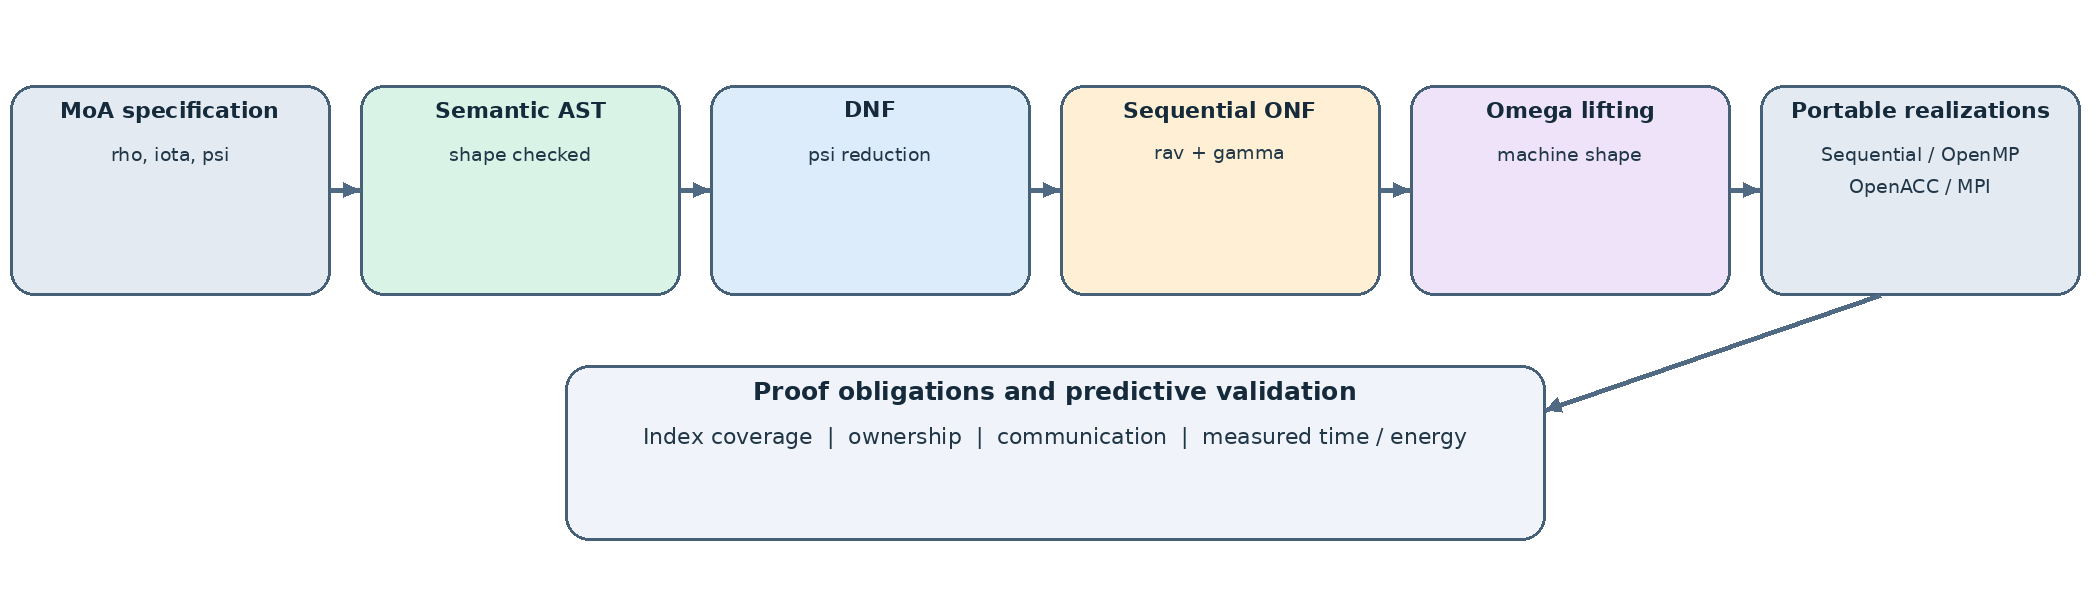
\includegraphics[width=.76\linewidth]{figure1_moa_pipeline.png}\caption{Proposed mechanized MoA transformation and validation path. $\psi$ reduction produces architecture-independent DNF; $\gamma$ addressing yields sequential ONF; $\Omega$ lifting changes execution shape. The machine descriptor enters the mapping and prediction stages.}\end{figure}
\section{Foundations: shape, index domain, and $\psi$}
For an array $A$, $\rho A$ is its shape, $\iota(\rho A)$ generates its valid index domain, and $\vec\imath\psisel A$ denotes $\psi$ selection. The element count and scalar dimensionality are
\begin{equation}
\tau(A)=\prod(\rho A),\qquad \delta(A)=\tau(\rho A).
\end{equation}
Index completeness is expressed as $(\iota(\rho A))\psisel A\equiv A$. These are properties of MoA arrays and not machine addresses. Vectors are rank-one arrays; matrices are rank-two arrays. Architecture-specific storage and traversal are introduced later.

\section{MoA all the way: the constructive proof architecture}
\label{sec:constructive}
The proposed compiler accepts a \emph{semantically defined array computation}, regardless of whether its source syntax originated in Fortran, MATLAB, Python, Julia, C, or another front end. A front end is responsible for preserving the defined meaning of the supported source-language subset; the common MoA machinery begins at that semantic boundary. Neither a language name nor a target instruction set appears in the mathematical DNF. Consequently, any supported source languages whose programs have the same defined array semantics obtain the same MoA DNF and the same mathematically derivable optimization opportunities; only their front-end representation and machine-specific realization differ.

Let $E$ be the MoA expression and $\mathcal R_\psi$ its index-composition rewrite relation. Write $E\rightarrow_\psi^*D$ for a finite sequence of $\psi$ reductions ending in DNF $D$. The Church--Rosser property means that diverging reductions can be joined; where the relevant reductions terminate in a unique canonical normal form, equivalent expressions have the same DNF. For MoA programs expressed over finite, shape-bounded index domains, the shape components supply the finite upper bounds on index composition and traversals. Thus the shape-bounded MoA reductions and computations considered here terminate; this statement concerns the defined MoA domain and does not assert termination of arbitrary unrestricted source-language control flow. We use Church--Rosser and the resulting common DNF as the mathematical equivalence criterion.
\begin{equation}
E_1\rightarrow_\psi^*D\quad\land\quad E_2\rightarrow_\psi^*D
\quad\Longrightarrow\quad E_1\equiv_{\rm MoA}E_2.
\label{eq:common-dnf}
\end{equation}
A machine description $\mathcal M$ supplies shaped resources and associated component values (capacities, hierarchy, transfer capabilities, costs, and constraints). For a feasible mapping $\mu$ the construction is
\begin{equation}
E\xrightarrow{\psi^*}D\xrightarrow{\text{1--1 indexed mapping}}\mathrm{ONF}_\gamma(D)
\xrightarrow{\Omega_\mu}\mathrm{ONF}_{\gamma,\mathcal M}^{\Omega}
\xrightarrow{\text{faithful instruction realization}}I_{\mathcal M}.
\label{eq:constructive}
\end{equation}
The proof is compositional: index composition establishes DNF; a layout function $\gamma$ represents the same indexed elements at addresses; $\Omega$ lifts and partitions those elements without omission or duplication; machine instructions implement the resulting ONF. Each arrow carries its own mathematical invariant. Thus \emph{specification proves realization} for supported mappings and instruction semantics by construction, rather than by comparing arbitrary optimized binaries after the fact. Floating-point reassociation, reduction order, exceptional values, and communication must be governed by an explicit numerical semantics or a stated error relation.

\section{A visible attention AST rewrite sequence}
\label{sec:ast-chain}
Consider one attention head with $\rho Q=\langle n,d\rangle$, $\rho K=\langle m,d\rangle$, $\rho V=\langle m,d_v\rangle$. The last-two-axis transpose is mandatory: $\rho(K^{T_{\rm last2}})=\langle d,m\rangle$. In particular,
\begin{equation}
\langle j,k\rangle\psi K^{T_{\rm last2}}=\langle k,j\rangle\psi K,
\qquad 0\le j<d,\;0\le k<m.
\label{eq:transpose-rule}
\end{equation}
This is a \emph{semantic} transpose rule, not an instruction to allocate a transposed copy. The small AST beside each mathematical stage is intended to make the corresponding hand derivation visually checkable. Figure~\ref{fig:ast-input} displays the original typed expression tree.
\begin{figure}[htbp]\centering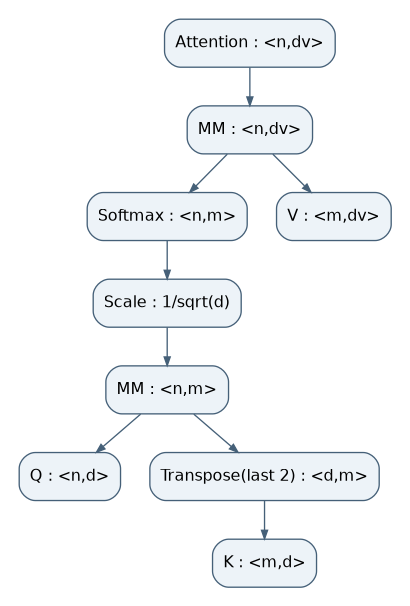
\includegraphics[width=.47\linewidth]{ast01_input.png}\caption{Beginning AST: attention as shape-checked array operators. The $K$ transpose changes its logical index order; its storage need not change.}\label{fig:ast-input}\end{figure}

Apply $\langle i,v\rangle\psi$ to the output, then recursively compose indices through matrix multiplication, transpose, scaling, and row normalization. For the score contraction the critical rewrite is
\begin{align}
\langle i,k\rangle\psi\bigl(Q\,\mathrm{MM}\,K^{T_{\rm last2}}\bigr)
&\rightarrow_\psi\sum_{j=0}^{d-1}(\langle i,j\rangle\psi Q)
(\langle j,k\rangle\psi K^{T_{\rm last2}})\\
&\rightarrow_\psi\sum_{j=0}^{d-1}(\langle i,j\rangle\psi Q)
(\langle k,j\rangle\psi K).
\label{eq:psi-mm}
\end{align}
The second arrow is index composition through transpose. It explains why, for fixed $i,k$ and row-major $Q,K$, both $j$-indexed operands are traversed contiguously. A different logical layout can be realized by a regular strided transfer when the machine supports it. The adjacent compact AST displays the intermediate $\psi$-indexed tree.\par\noindent\begin{minipage}[c]{.57\linewidth}\small\textbf{Indexed contraction:}\quad $s(i,k)=d^{-1/2}\sum_j Q[i,j]K[k,j]$.\end{minipage}\hfill\begin{minipage}[c]{.37\linewidth}\centering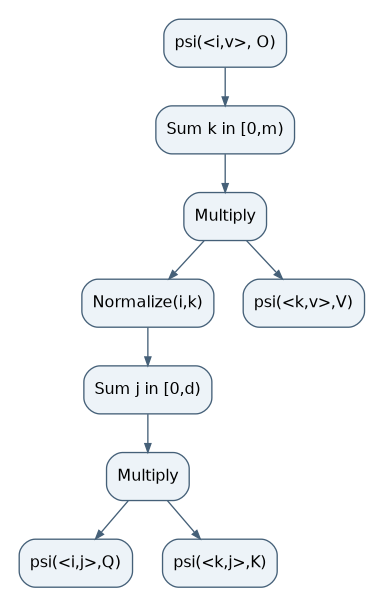
\includegraphics[width=\linewidth]{ast02_psi.png}\end{minipage}\par


\subsection{Cartesian-indexed DNF: the end of semantic reduction}
The result is not merely a loop nest: it is a function on a Cartesian index domain. With $\mathcal I=\{(i,k,j,v)\mid 0\le i<n,\,0\le k<m,\,0\le j<d,\,0\le v<d_v\}$, define
\begin{align}
s(i,k)&=\frac{1}{\sqrt d}\sum_{j=0}^{d-1}(\langle i,j\rangle\psi Q)(\langle k,j\rangle\psi K),\\
a(i)&=\max_{0\le k<m}s(i,k),\qquad z(i)=\sum_{k=0}^{m-1}e^{s(i,k)-a(i)},\\
\langle i,v\rangle\psi O&=\sum_{k=0}^{m-1}\frac{e^{s(i,k)-a(i)}}{z(i)}(\langle k,v\rangle\psi V).
\label{eq:cartesian-dnf}
\end{align}
All domains, shapes, and selections are explicit. This is the architecture-independent reference to which the subsequent operational forms must correspond. The adjacent compact AST displays the end of $\psi$ reduction.\par\noindent\begin{minipage}[c]{.55\linewidth}\small\textbf{DNF:} each output $\langle i,v\rangle\psi O$ is determined by the displayed Cartesian-indexed sums, maxima, and selections.\end{minipage}\hfill\begin{minipage}[c]{.39\linewidth}\centering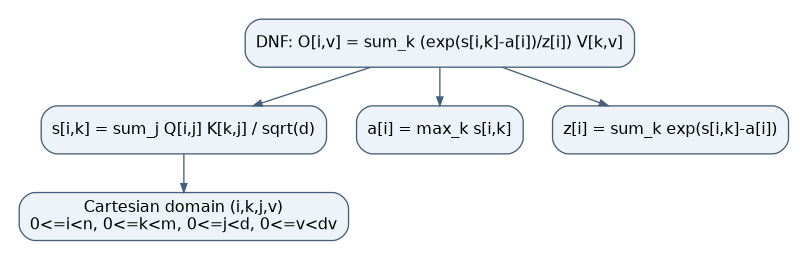
\includegraphics[width=\linewidth]{ast03_dnf.png}\end{minipage}\par


\subsection{DNF to sequential ONF: addressing is the realization}
For a layout family $\gamma_{\lambda}$ (row-major, column-major, or another supported layout), addressing is a function of an index and the \emph{shape of the indexed array}:
\begin{equation}
\vec\imath\psi X=(\operatorname{rav}X)[\gamma_{\lambda}(\vec\imath;\rho X)].\label{eq:gamma-family}
\end{equation}
For row-major arrays, $\gamma_{\rm row}(\langle i,j\rangle;\langle n,d\rangle)=id+j$ and $\gamma_{\rm row}(\langle k,j\rangle;\langle m,d\rangle)=kd+j$. In contrast, $\gamma_{\rm col}(\langle i,j\rangle;\langle n,d\rangle)=i+nj$. In particular $\langle k,j\rangle\psi K=(\operatorname{rav}K)[\gamma_{\rm row}(\langle k,j\rangle;\rho K)]$. For fixed $k$, its $j$ sequence has $(\mathrm{start},\mathrm{stop},\mathrm{stride})=(kd,(k+1)d,1)$ in elements (exclusive stop). The corresponding $Q$ sequence is $(id,(i+1)d,1)$. Other valid mappings can derive a regular nonunit stride and use supported DMA, vector, or hierarchical transfers; contiguity is a useful cost characteristic, not an axiom of universal optimality.
\begin{figure}[htbp]\centering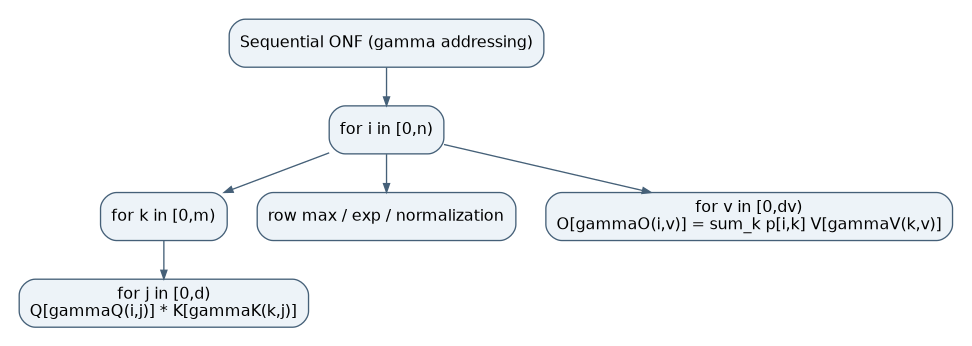
\includegraphics[width=.48\linewidth]{ast04_onf.png}\caption{Sequential ONF AST: the DNF's exact index selections become $\gamma$-addressed operations. Loop ordering is a mapping choice; the Cartesian-indexed DNF remains unchanged.}\label{fig:ast-onf}\end{figure}

\subsection{Sequential to parallel and distributed ONF by dimension lifting}
Let $L=\lceil n/P\rceil$ and $I_p=\{pL+u\mid 0\le u<L,\;pL+u<n\}$. For $n>0$ and $P>0$,
\begin{equation}
\{0,\ldots,n-1\}=\biguplus_{p=0}^{P-1}I_p.
\label{eq:coverage-lift}
\end{equation}
The quotient--remainder decomposition proves unique ownership of each output query $i$. A scheduling function $\sigma(p)$ assigns logical partitions to workers; $P$ need not equal the number of threads, GPUs, or nodes. The same lifted ONF can therefore be realized as an OpenMP loop, a GPU grid, an MPI partition, or a heterogeneous assignment without altering DNF.

If $K,V$ are replicated, each query owner can compute its output independently. If keys and values are sharded, the score maximum, exponential denominator, and weighted numerator require communication. For disjoint key shards $H_r$, define local stable summaries $(a_r,z_r,u_{r,v})$ where $a_r=\max_{k\in H_r}s(i,k)$, $z_r=\sum_{k\in H_r}e^{s(i,k)-a_r}$, and $u_{r,v}=\sum_{k\in H_r}e^{s(i,k)-a_r}(\langle k,v\rangle\psi V)$. Combining two summaries gives
\begin{align}
a&=\max(a_1,a_2),\\
z&=e^{a_1-a}z_1+e^{a_2-a}z_2,\\
u_v&=e^{a_1-a}u_{1,v}+e^{a_2-a}u_{2,v},\qquad O[i,v]=u_v/z.
\label{eq:distributed-merge}
\end{align}
This composition reproduces the global stable-normalization formula in exact arithmetic and permits a tree reduction across distributed resources. Floating-point reproducibility and exceptional cases require explicit conventions. The mapping must also establish the placement and transfer of $Q,K,V$ across memory levels, and ensure each output is written exactly once.
\begin{figure}[htbp]\centering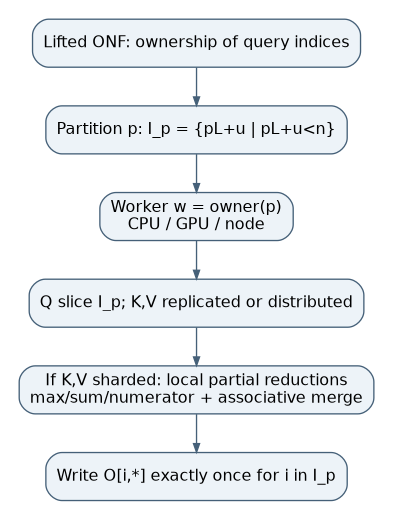
\includegraphics[width=.49\linewidth]{ast05_lift.png}\caption{Lifted ONF AST: the Cartesian query domain becomes disjoint ownership domains; the machine-shape mapping chooses CPU, GPU, and distributed workers. Replication or sharding of $K,V$ determines whether distributed summary reductions are needed.}\label{fig:ast-lift}\end{figure}

\subsection{Constructive equivalence and performance selection}
The proof obligation is a commuting correspondence: every $\psi$ selection in DNF is realized by exactly the appropriate $\gamma$-addressed value, every output index belongs to one lifted owner, and any distributed reduction implements the same mathematical reduction. The generated instructions must faithfully implement the lifted ONF. These are proof obligations of the construction, not experimental claims. Among mappings satisfying them and the resource constraints, the compiler can compare predicted time and energy, potentially identifying a Pareto frontier rather than a single simultaneously optimal mapping. Measured runtime and energy remain necessary to validate physical predictions.

\section{Worked attention expression and AST}
Let $\rho Q=\langle B,N,D\rangle$, $\rho K=\langle B,N,D\rangle$, and $\rho V=\langle B,N,D_v\rangle$. A representative attention expression has indexed scores, stable probabilities, and output
\begin{align}
S_{b,i,j}&=D^{-1/2}\sum_{d=0}^{D-1}(\langle b,i,d\rangle\psisel Q)(\langle b,j,d\rangle\psisel K),\\
m_{b,i}&=\max_{0\le j<N}S_{b,i,j},\\
P_{b,i,j}&=\frac{\exp(S_{b,i,j}-m_{b,i})}{\sum_{k=0}^{N-1}\exp(S_{b,i,k}-m_{b,i})},\\
\langle b,i,v\rangle\psisel O&=\sum_{j=0}^{N-1}P_{b,i,j}(\langle b,j,v\rangle\psisel V).
\end{align}
This is an explanatory indexed expansion of the attention semantics. Section~\ref{sec:paper1} develops the explicit component equations and a row-fused ONF using the available SC27 derivation source. The current baseline generator still materializes probabilities and a score workspace.
\begin{figure}[htbp]\centering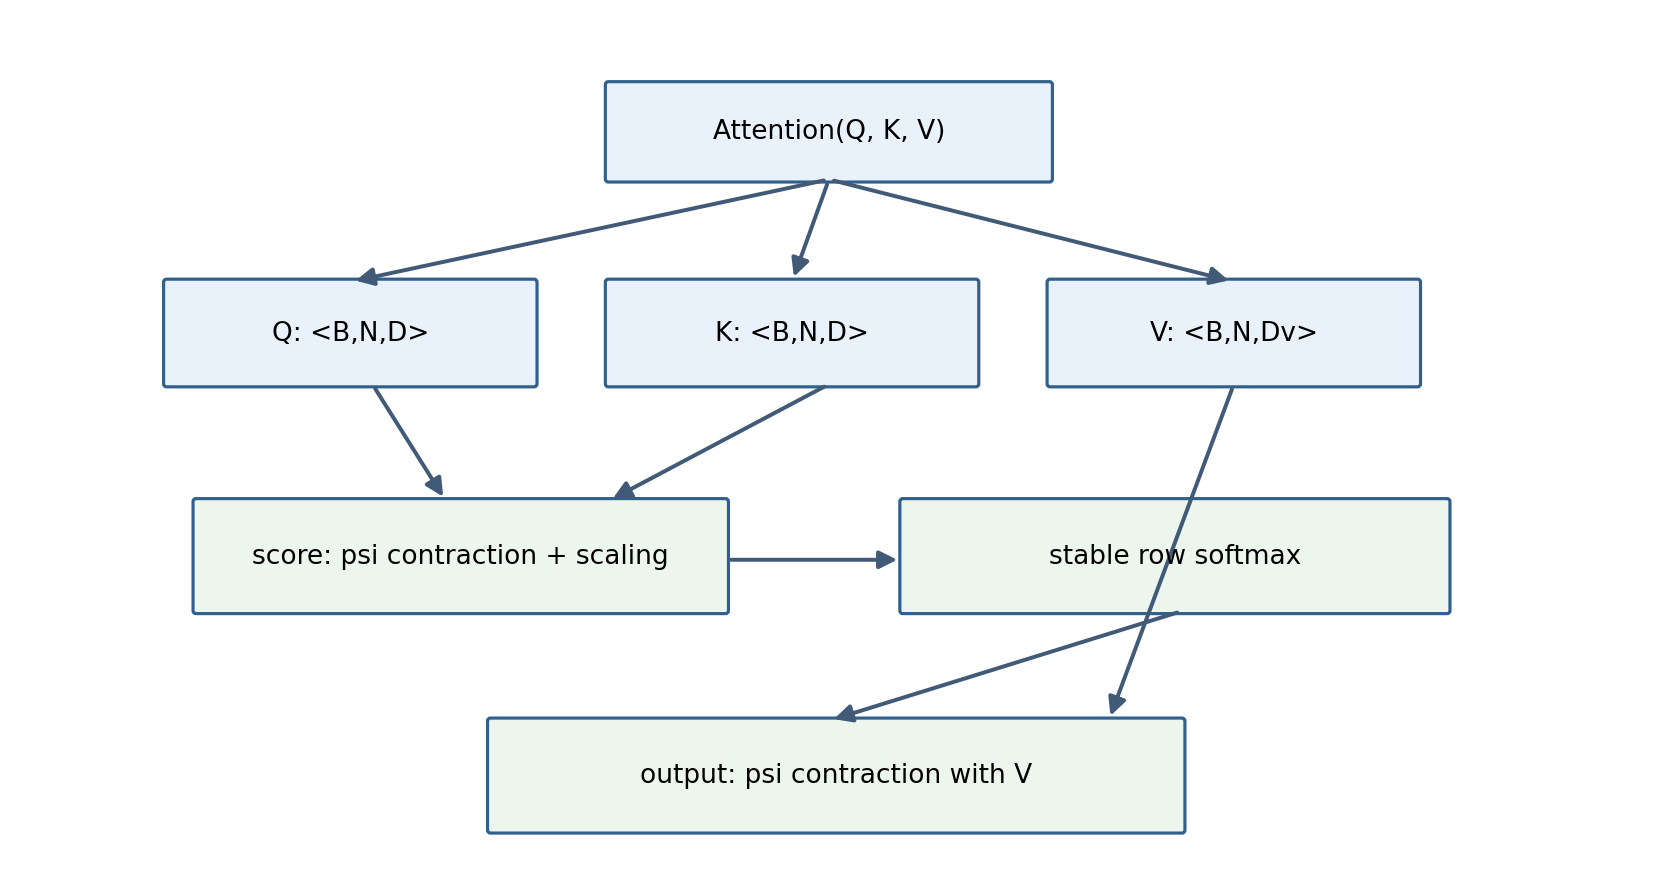
\includegraphics[width=.53\linewidth]{figure2_attention_ast.png}\caption{Schematic attention semantic AST: shaped inputs, $\psi$-based contraction, stable normalization, and output contraction. The production compiler diagram should enumerate actual AST node types and rewrite rules.}\end{figure}

\section{Paper 1 mathematical path: input expression to reduced DNF}
\label{sec:paper1}
This section makes the attention derivation explicit rather than treating the computation as a black-box library call. The equations are grounded in the worked attention derivation in the earlier MoA attention derivation and SC27 working source used in preparing this draft. They are \emph{not} presented as a verbatim transcription of the arXiv source; final notation and code alignment should be checked against the authoritative Paper~1 submission before publication.

\subsection{Input array expression and typed semantic AST}
For single-head unmasked attention, set $\rho Q=\langle n,d_k\rangle$, $\rho K=\langle m,d_k\rangle$, $\rho V=\langle m,d_v\rangle$, and $\rho O=\langle n,d_v\rangle$. The input expression is
\begin{equation}
O=\operatorname{softmax}(QK^{\mathsf T}/\sqrt{d_k})V.
\label{eq:surface}
\end{equation}
The transpose in this surface expression is a semantic access transformation, not a requirement to materialize a transposed array. An AST must carry shapes and index extents at each node: $\mathrm{Attention}(\mathrm{Softmax}(\mathrm{Scale}(\mathrm{Contract}(Q,\mathrm{Transpose}(K)))),V)$, with well-formedness constraints $\rho Q[1]=\rho K[1]$ and $\rho K[0]=\rho V[0]$. Figure~\ref{fig:rewrite} displays the rewrite stages.

\subsection{$\psi$-reduced component semantics}
Applying $\psi$ to the score expression makes the contraction and its valid domain explicit:
\begin{equation}
s_{ik}=d_k^{-1/2}\sum_{j=0}^{d_k-1}
(\langle i,j\rangle\psisel Q)(\langle k,j\rangle\psisel K),
\quad 0\le i<n,\;0\le k<m.
\label{eq:score-dnf}
\end{equation}
Stable normalization is given by
\begin{equation}
a_i=\max_{0\le k<m}s_{ik},\qquad
z_i=\sum_{k=0}^{m-1}\exp(s_{ik}-a_i),
\label{eq:stable-dnf}
\end{equation}
and the output by
\begin{equation}
\langle i,v\rangle\psisel O
=\sum_{k=0}^{m-1}\frac{\exp(s_{ik}-a_i)}{z_i}
(\langle k,v\rangle\psisel V),\qquad 0\le v<d_v.
\label{eq:output-dnf}
\end{equation}
Equations~\eqref{eq:score-dnf}--\eqref{eq:output-dnf} specify the architecture-independent component computation. They expose precisely which $Q$, $K$, and $V$ elements are required and permit rectangular $n\ne m$ inputs. The maximum subtraction is algebraically neutral over exact real arithmetic but floating-point evaluation requires a stated tolerance and reduction-order policy.

\subsection{A fused, memory-reduced operational derivation}
A score matrix of shape $\langle n,m\rangle$ contains $nm$ elements; separately materialized probabilities require another $nm$ elements. For one query $i$, however, Eqs.~\eqref{eq:score-dnf}--\eqref{eq:output-dnf} depend only on the $m$ scores for that query. Therefore a sequential ONF can calculate $s_{i0},\ldots,s_{i,m-1}$ in an $m$-element scratch array, compute $a_i,z_i$, and accumulate the $d_v$ output components without storing the full $n\times m$ score or probability arrays. In fp64 the score scratch is $8m$ bytes per concurrently processed query, apart from runtime overhead and output storage. This is the reference \emph{row-fused} memory bound; it must not be confused with a proof of the globally minimal memory bound for every attention variant.

An additional algebraic option, which must be checked against the specific Paper~1 code before being attributed to that implementation, is an online stable normalization. Define $m_r=\max_{0\le k<r}s_{ik}$, $\ell_r=\sum_{k<r}\exp(s_{ik}-m_r)$, and $u_{r,v}=\sum_{k<r}\exp(s_{ik}-m_r)(\langle k,v\rangle\psisel V)$. When score $s_{ir}$ arrives, with $m'=\max(m_r,s_{ir})$, update
\begin{align}
\ell_{r+1}&=e^{m_r-m'}\ell_r+e^{s_{ir}-m'},\\
u_{r+1,v}&=e^{m_r-m'}u_{r,v}+e^{s_{ir}-m'}(\langle r,v\rangle\psisel V).
\end{align}
The invariant follows by factoring $e^{-m'}$ from the sum over the first $r+1$ scores. After processing all $m$ keys, $\langle i,v\rangle\psisel O=u_{m,v}/\ell_m$. This alternative avoids an $m$-score scratch array but has distinct numerical and implementation characteristics; it is shown as a derivable transformation, not as an assertion about the current compiler's generated kernel.

\subsection{DNF to $\gamma$-addressed sequential ONF}
For row-major storage, the shape-dependent addressing instances are
\begin{align}
\gamma_{\rm row}(\langle i,j\rangle;\rho Q)&=i d_k+j, &\gamma_{\rm row}(\langle k,j\rangle;\rho K)&=k d_k+j,\\
\gamma_{\rm row}(\langle k,v\rangle;\rho V)&=k d_v+v, &\gamma_{\rm row}(\langle i,v\rangle;\rho O)&=i d_v+v.
\end{align}
Then $(\langle i,j\rangle\psisel Q)$ is realized as $(\operatorname{rav}Q)[\gamma_{\rm row}(\langle i,j\rangle;\rho Q)]$, and similarly for the other arrays. This changes the realization, not the DNF's index semantics. The sequential ONF loops over $i$, then $k,j$ to form scores, reduces the row maximum and denominator, and loops over $v,k$ to produce each output. The row-fused realization retains only one query's score scratch at a time.

\subsection{Lifted ONF, exact coverage, and resource allocation}
Partition query indices into $P$ nonoverlapping domains $I_p$ satisfying $\biguplus_{p=0}^{P-1}I_p=\{0,\ldots,n-1\}$. For the concrete contiguous partition rule $L=\lceil n/P\rceil$, let $I_p=\{pL+u\mid 0\le u<L,\;pL+u<n\}$. Every valid query index occurs in exactly one domain because Euclidean quotient and remainder with divisor $L$ are unique. This establishes query ownership; preservation of score reductions, scratch ownership, and output writes must also be verified. The number of partitions $P$ is independent of the number of OpenMP threads $T$. A resource model must account for at least $T$ concurrent scratch arrays of length $m$ for a thread-local row-fused implementation, and for communication when $K,V$ are distributed.

\begin{figure}[htbp]\centering
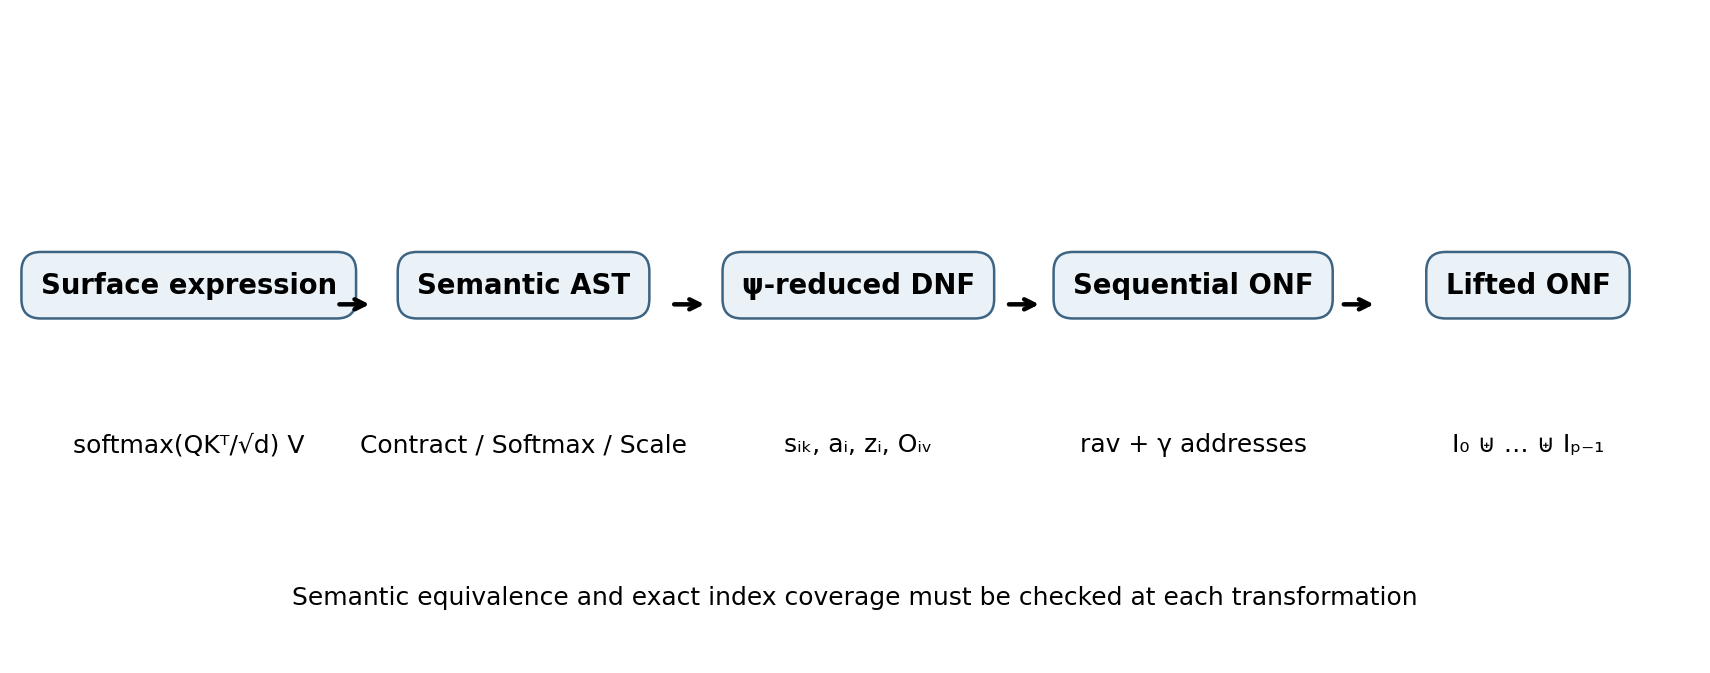
\includegraphics[width=.62\linewidth]{figure6_paper1_rewrite.png}
\caption{Detailed attention rewrite chain: the surface expression becomes a shaped semantic AST; $\psi$ reduction exposes exact component dependencies; the DNF is realized with $\gamma$ addresses and then lifted to disjoint query partitions. The diagram is a conceptual transformation trace, not an export of the compiler's internal AST.}\label{fig:rewrite}
\end{figure}

\subsection{Compiler acceptance test against the hand derivation}
For every supported input shape, a compiler-generated ONF must match the independently implemented $\psi$-indexed DNF and hand-derived ONF within a declared floating-point criterion. The compiler must also report the exact covered query domain, per-partition work, temporary allocation, and machine mapping. Only after those checks should predicted time, power, and energy be evaluated on held-out hardware configurations. In particular, the v13 DGX predictor reported later in this paper measures a materializing baseline; it is \emph{not} a performance result for the row-fused or online-memory-reduced realization above.

\section{$\psi$ reduction, DNF, and sequential ONF}
$\psi$ reduction makes the index domain and element dependencies explicit. DNF fixes the computation independent of storage layout and processor allocation. For a row-major operational realization, $\gamma$ can map a three-dimensional array index to an address offset:
\begin{equation}
\gamma_{\rm row}(\langle b,i,d\rangle;\rho Q)=((bN+i)D+d),\quad \langle b,i,d\rangle\psisel Q=(\operatorname{rav}Q)[\gamma_{\rm row}(\langle b,i,d\rangle;\rho Q)].
\end{equation}
For example, the ONF for an output element uses $(\operatorname{rav}O)[\gamma_{\rm row}(\langle b,i,v\rangle;\rho O)]\leftarrow\sum_j(\operatorname{rav}P)[\gamma_{\rm row}(\langle b,i,j\rangle;\rho P)](\operatorname{rav}V)[\gamma_{\rm row}(\langle b,j,v\rangle;\rho V)]$, subject to the full preceding definitions of $P$. This address translation does not alter the DNF's meaning. The generated sequential code is then the baseline against which lifted implementations are checked.
\section{Dimension lifting and shaped execution}
For a query domain $I=\{0,\ldots,N-1\}$, a valid lifted partition must satisfy
\begin{equation}I=\biguplus_{p=0}^{P-1}I_p,\qquad I_p\cap I_q=\varnothing\quad(p\ne q).\end{equation}
A concrete quotient/remainder construction may use $L=\lceil N/P\rceil$ and $i=pL+u$, with $0\le p<P$, $0\le u<L$, and the guard $i<N$. This proves coverage and disjointness of valid query indices. The partition count $P$ is not the number of OpenMP threads $T$: multiple partitions can be scheduled by one thread.
\begin{figure}[htbp]\centering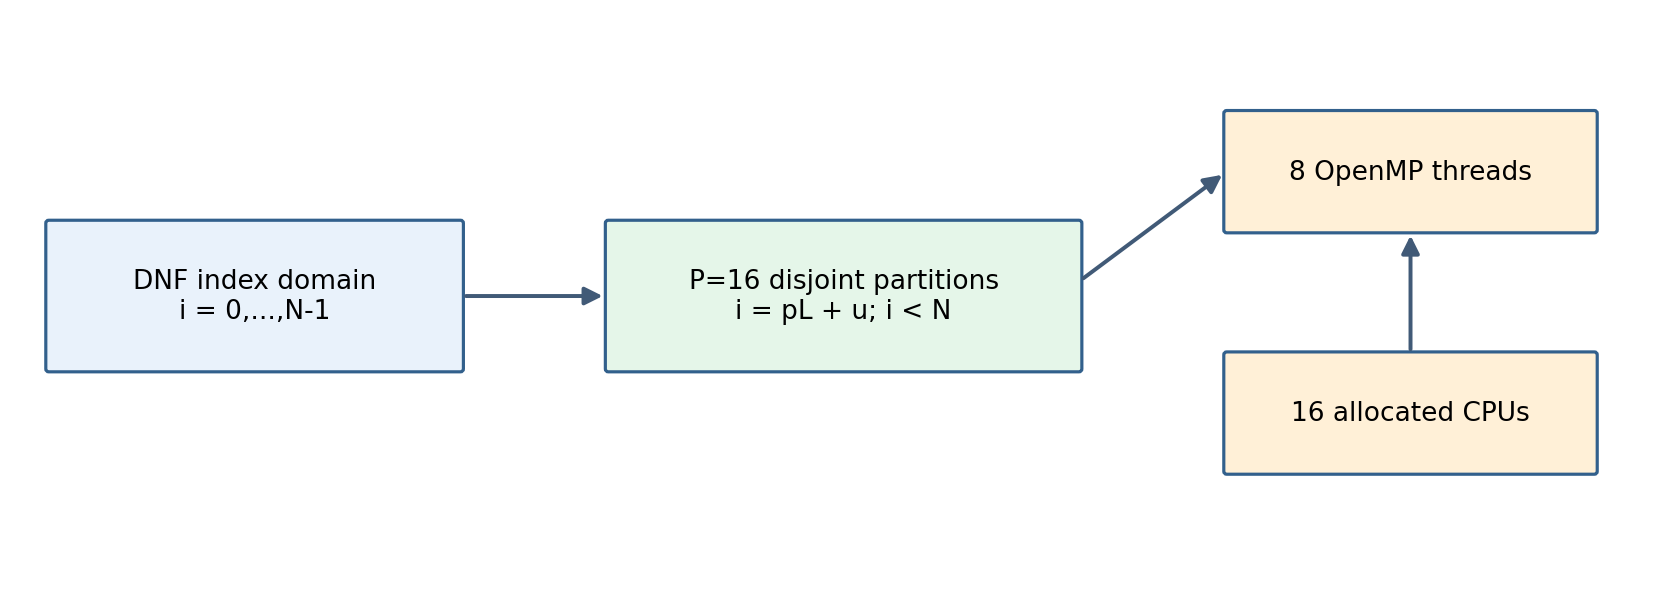
\includegraphics[width=.65\linewidth]{figure5_lifting.png}\caption{Query-domain lifting in the tested attention implementation. Sixteen logical partitions were executed with eight OpenMP threads inside a sixteen-logical-CPU Slurm allocation. This does not establish that sixteen-thread execution is slower; that configuration has not yet been tested.}\end{figure}
\section{Machine shape and prediction obligations}
The deterministic machine-shape descriptor is under development as a ten-field characterization: compute units $U$, warp width $W$, shared memory $M$, measured reference time $t$, measured memory ceiling $n_{\max}$, total memory capacity $M_{\mathrm{cap}}$, realization power $P$, execution-unit reachability $X$, compiler-directive configuration $C$, and reservation overhead $R$. Some fields are measured or realization-specific, so a deterministic machine shape does not automatically imply an analytically exact runtime prediction. The provisional CPU-only \texttt{MachineShape10} in the repository is a distinct implementation interface and must not be conflated with this research descriptor.

The current baseline attention kernel has source-level persistent arrays $Q,K,V,P,O$ and a full score workspace. For 64-bit elements the corresponding source-level allocation model is
\begin{equation}M_{\mathrm{alloc}}=8B(2ND+2ND_v+2N^2),\end{equation}
excluding allocator, runtime, and other transient overhead. The arithmetic multiplication count for the baseline score and output contractions is $W=B N^2(D+D_v)$. The current empirical predictor fits $\widehat{T}=\alpha+\beta W_{\mathrm{critical}}$ for each mapping, with $W_{\mathrm{critical}}$ estimated from static partition work. This is not yet a closed-form machine-shape-derived time model.
\section{UAlbany DGX held-out attention validation}
The experiment ran on \texttt{dgx03}, an AMD EPYC 7742 compute node, with a Slurm allocation of 16 logical CPUs and GCC 11.4.0 using \texttt{-O2 -fopenmp}. The measured affinity list was \texttt{60-63,124-127,188-191,252-255}. Double-precision baseline attention used $B=1$, $D=D_v=32$. The calibration lengths were $N\in\{96,160,256\}$, and the unseen holdouts were $N\in\{320,448\}$. Each case used nine timed samples after four warmups. All reported $P$ and $O$ correctness errors were zero at the printed precision.
\begin{figure}[htbp]\centering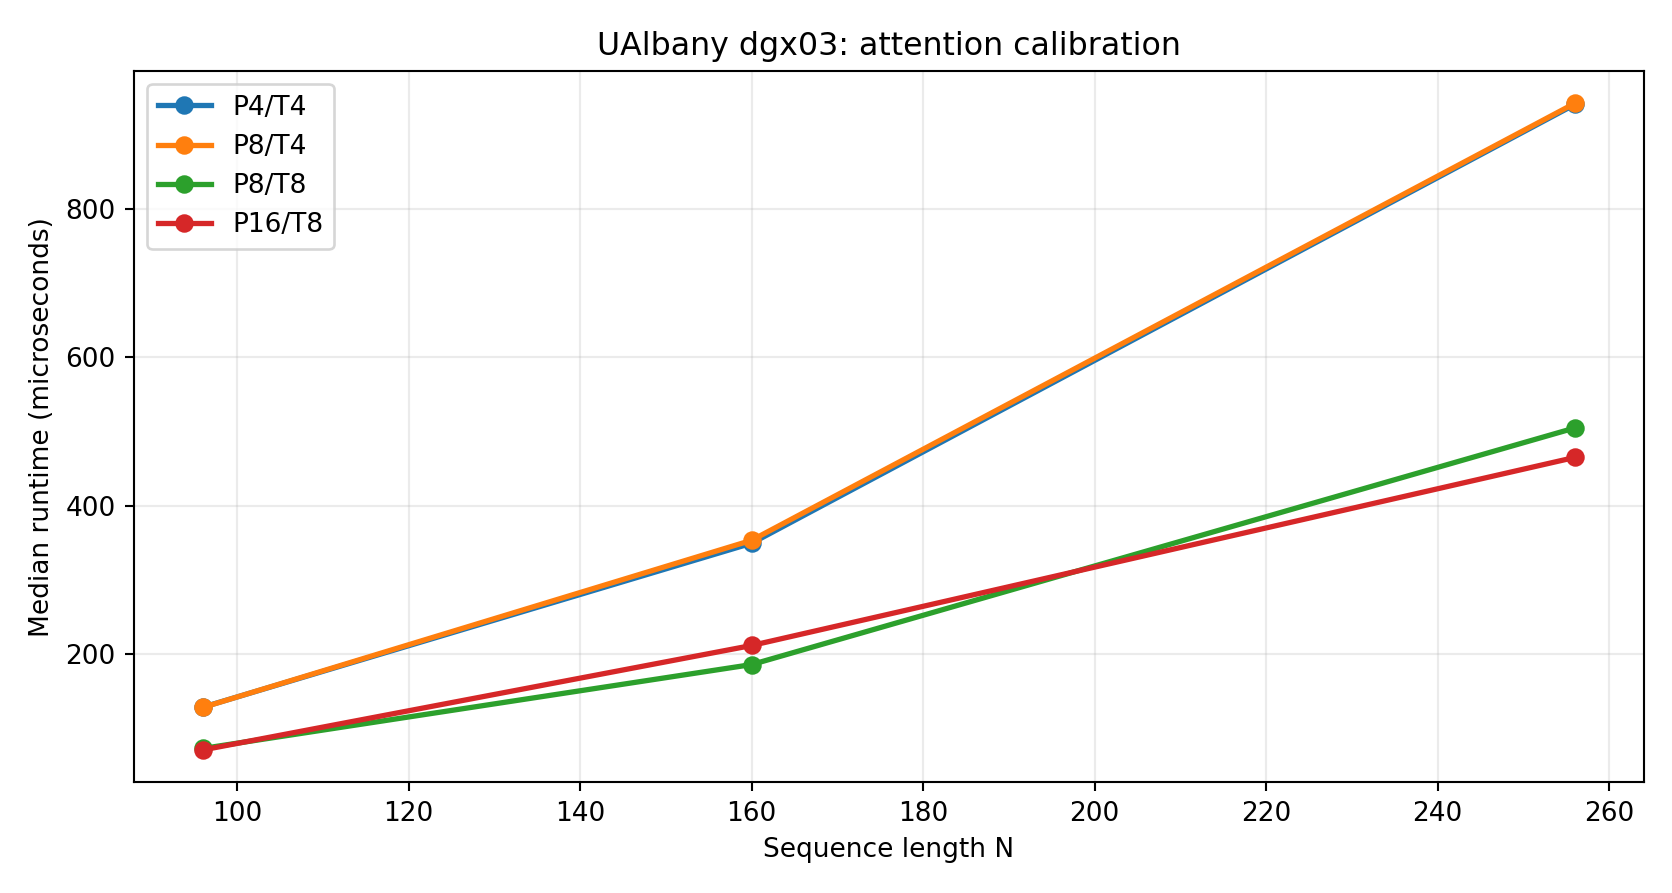
\includegraphics[width=.63\linewidth]{figure3_calibration.png}\caption{Measured calibration medians for the four partition/thread candidates. The legend distinguishes partitions $P$ from threads $T$.}\end{figure}
\begin{table}[htbp]\centering\caption{Frozen-prediction validation, selected mapping $P=16$, $T=8$.}\begin{tabular}{rrrrr}\toprule $N$ & Predicted ($\mu$s) & Measured ($\mu$s) & Abs. error & Selection regret\\\midrule 320 & 723.635 & 722.060 & 0.22\% & 0\%\\448 & 1400.348 & 1471.371 & 4.83\% & 0\%\\\bottomrule\end{tabular}\end{table}
\begin{figure}[htbp]\centering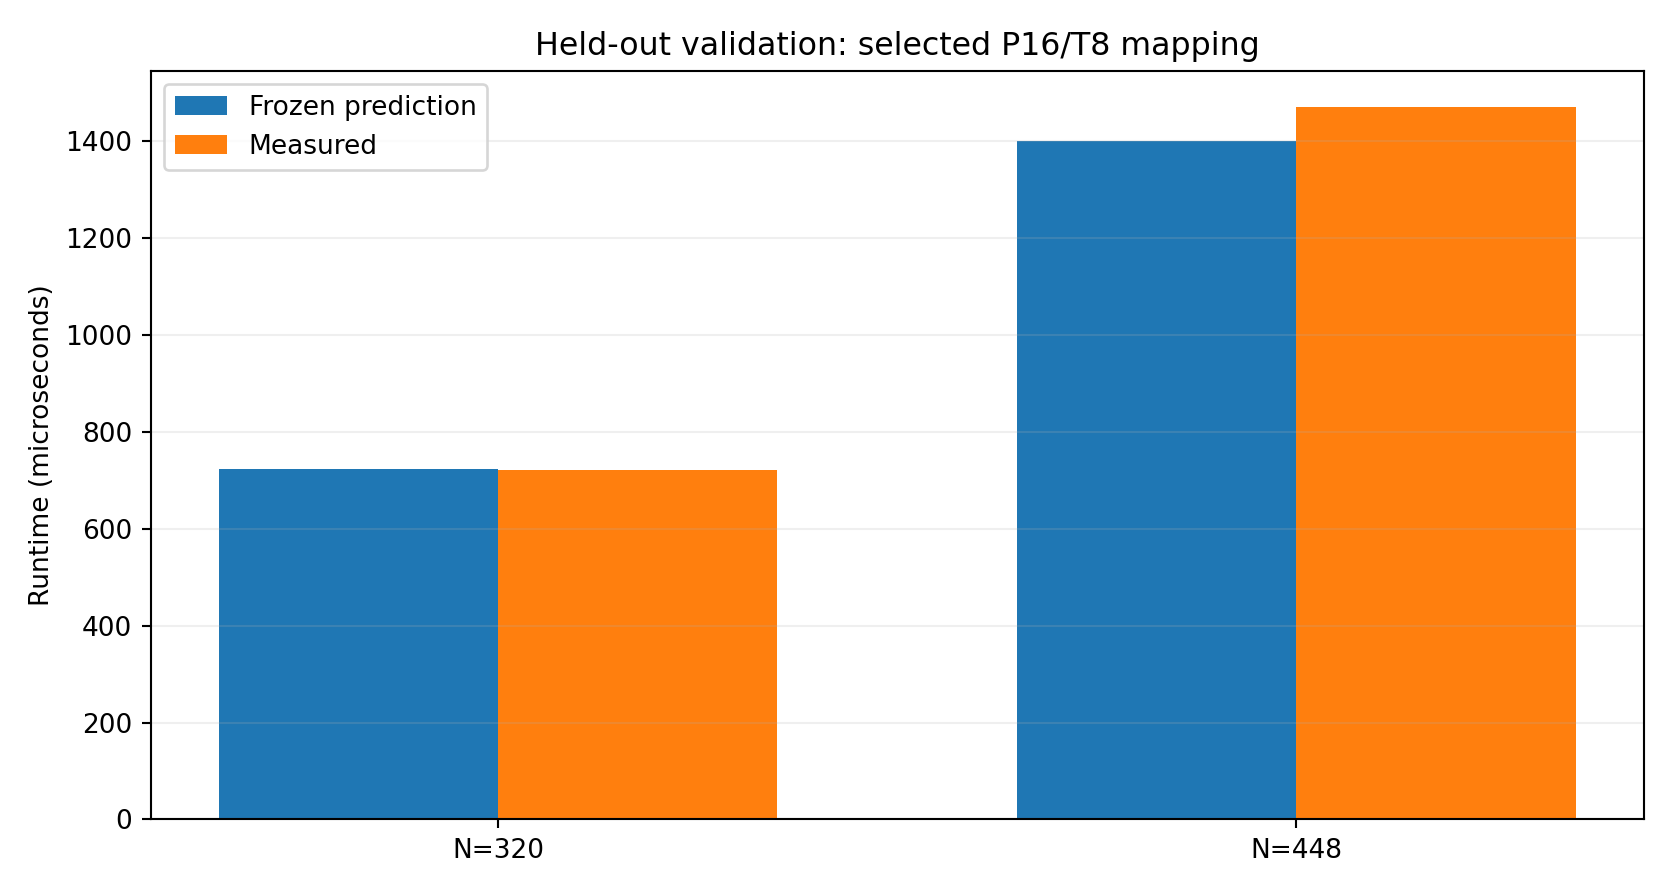
\includegraphics[width=.66\linewidth]{figure4_holdout.png}\caption{Frozen versus observed times for the selected mapping. Both selections were fastest among the four measured candidates, not necessarily globally optimal.}\end{figure}
The prediction certificate was frozen before validation with SHA-256 \texttt{a73981eb98d7f8858b9676168a86369a334092693005e33ef8b4b196b5923e2d}. The measured candidate times at $N=320$ were 1482.522, 1429.852, 727.610, and 722.060 $\mu$s; at $N=448$ they were 2929.547, 2919.638, 1477.623, and 1471.371 $\mu$s, respectively, in candidate order $(4,4),(8,4),(8,8),(16,8)$. The $N=448$ difference between the two eight-thread mappings is small; repeated runs and placement controls are needed to assess selection stability.
\section{Mechanization milestones and limitations}
The compiler must (i) preserve the shaped semantics of the input AST, (ii) produce a verifiable $\psi$-reduced DNF, (iii) map DNF one-to-one to sequential ONF with explicit $\gamma$, (iv) produce lifted ONFs whose index sets form an exact disjoint cover, (v) predict resource requirements from the shaped computation and target, and (vi) compare frozen performance predictions against measurements. The present attention timing model is empirical; its thread-load assignment approximates OpenMP static scheduling and does not independently identify memory, synchronization, or affinity costs. The present generated attention kernel is not the full memory-optimal Paper~1 implementation. A separate experiment must compare eight and sixteen OpenMP threads before asserting that the remaining eight allocated CPUs are redundant; subsequent experiments may test two concurrent eight-thread workloads and aggregate throughput.

\section{MoA as a unified mathematics of computation, machines, and prediction}
The long-term objective is not simply to compile one attention kernel for one processor. It is to derive, within MoA, semantically equivalent executable implementations for diverse configurations of coordinated heterogeneous resources and select a feasible mapping that optimizes execution time and energy according to an explicit objective. The computation and the available machine resources are both represented as shaped structures. MoA transformations are required to preserve the meaning of the computation while refining the operational placement, communication, and traversal of its elements.

Let $E$ denote the input MoA expression, $D(E)$ its $\psi$-reduced DNF, and $\mathcal{M}$ a description of the available resource ensemble. For each feasible configuration $c\in\mathcal{C}(\mathcal{M})$, let $G(D(E),c)$ be generated executable code. The primary semantic obligation is
\begin{equation}
\operatorname{Sem}(G(D(E),c))\equiv\operatorname{Sem}(E),\qquad c\in\mathcal{C}(\mathcal{M}),
\end{equation}
where equivalence for floating-point programs must specify the arithmetic model, reduction order, and acceptable numerical tolerance. The compiler's search must also enforce memory capacity, index-domain coverage, data-dependency, reachability, and communication constraints. Thus semantic equivalence is not a consequence of measured speed; it is a separate proof obligation.

Time and energy are competing objectives. A precise statement of the design goal is to identify feasible nondominated configurations
\begin{equation}
\mathcal{P}=\left\{c\in\mathcal{C}(\mathcal{M}):\nexists c'\in\mathcal{C}(\mathcal{M})\text{ with }T(c')\le T(c),\ E(c')\le E(c)\text{ and one strict}\right\},
\end{equation}
or minimize time subject to an energy budget (or vice versa). Here $T$ and $E$ are machine-dependent quantities that must be predicted and subsequently measured; neither is established solely by algebraic operation counts. The eventual compiler should generate independently checkable semantic and resource certificates and report uncertainty or error for physical predictions.

\section{MoA all the way: four-paper compiler reproduction contract}
\label{sec:fourpapercontract}
The governing acceptance criterion is stronger than generating a numerically plausible attention kernel. For each of the four independently hand-derived research programs, the compiler must mechanically reproduce a traceable MoA derivation, an executable realization, and an independently testable prediction. The hand-derived programs and their published measurements are \emph{reference evidence}, not compiler-generated results. No row/column-vector reinterpretation or architecture-specific intermediate mathematics is introduced: arrays retain their MoA shapes, and machine resources are shaped arrays too.

For each reference program $p$, let $E_p$ be its shaped MoA specification, $D_p$ the verified $\psi$-reduced DNF, $O_p$ the $\gamma$-addressed ONF, and $L_p(\mathcal M)$ the $\Omega$-lifted ONF on shaped machine $\mathcal M$. The compiler's reproduction obligation is the certified chain
\[
E_p \xRightarrow{\psi} D_p
\xRightarrow{\gamma,\operatorname{rav},[\,]} O_p
\xRightarrow{\Omega,\rho\mathcal M} L_p(\mathcal M)
\longrightarrow G_p(\mathcal M),
\]
with index-domain coverage, dependency preservation, legal ownership or reduction, resource feasibility, and a specified floating-point relation checked at each relevant transition. Before executing $G_p$, a machine-shape-based prediction and its assumptions must be frozen; measured results are then compared against that prediction and against the hand-derived reference. Numerical equivalence alone does not certify equivalent storage, communication, or predictive behavior.

\begin{table}[htbp]\centering\small
\caption{Four-paper reproduction contract. Entries describe required evidence, not completed compiler capabilities.}\label{tab:fourpapercontract}
\begin{tabular}{p{0.18\linewidth}p{0.36\linewidth}p{0.36\linewidth}}\toprule
Hand-derived reference & MoA derivation and machine obligations & Reproduction evidence required \\\midrule
Forward attention (Paper 1) & Score contraction, stable normalization, value contraction; DNF/ONF, scratch elimination, $\Omega$ ownership & Generated full forward kernel, numerical and address checks, allocation/traffic certificate, frozen predictions \\
Backward attention (Paper 2) & Gradient dependencies and reductions; legal accumulation, addressing, and partitioning & Generated backward kernel, gradient reference comparison, reduction/communication certificate, frozen predictions \\
Decode attention (Paper 3) & KV-cache indexing, GQA/MQA shape relationships, cache ownership, OpenACC realization & Generated decode kernel, cache/index checks, transfer/communication accounting, frozen predictions \\
Transformer block (Paper 4) & RMSNorm, attention, gated feed-forward composition and fusion; intermediate lifetimes & Generated complete block, stagewise/end-to-end checks, storage and communication certificates, frozen predictions \\\bottomrule
\end{tabular}
\end{table}

A pass is recorded only when the compiler artifacts and independent verification logs are archived for the same specification, shape, numerical contract, and machine configuration as the hand-derived reference. Existing component regression tests are evidence for their \emph{individual} obligations; they do not automatically promote any of the four rows to end-to-end reproduced status. The first integration target is complete forward attention; subsequent targets extend the same MoA chain rather than introducing new foundations for backward, decode, or block execution.

\section{Experimental lineage and resource provenance}
The research sequence is theory first: formulate attention in MoA; perform $\psi$ reduction; derive the DNF and ONF by hand; dimension-lift onto a target machine; implement; measure; and use discrepancies to refine the machine description. The current compiler effort seeks to mechanize this established manual sequence. The earlier implementations should not be described as compiler-generated.
\begin{table}[htbp]\centering\small
\caption{Research resources and their distinct roles. Individual configurations, award identifiers, and measured outcomes require cross-reference to the corresponding experiment logs and publications.}
\begin{tabular}{p{0.26\linewidth}p{0.64\linewidth}}\toprule
Resource & Research role \\\midrule
Stampede, Expanse, Bridges & ACCESS-supported heterogeneous performance research and hand-derived implementation studies.\\
Purdue Anvil & ACCESS execution and validation of hand-derived MoA algorithms.\\
NCSA Delta (including AMD GPU) & Accelerator experiments, including AMD GPU execution.\\
Chameleon Cloud (separate award) & Intel GPU energy experiments, separate from the ACCESS resource allocation.\\
University at Albany DGX & Present compiler-generated CPU attention calibration and frozen holdout validation.\\
\bottomrule\end{tabular}\end{table}

\section{Coordinated heterogeneous resource allocation}
A heterogeneous resource ensemble can include CPU cores, GPU execution units, local and remote memories, network links, and communication/synchronization mechanisms. A machine-shape representation must encode the capacities and access relations relevant to a particular mapping. The compiler should derive partitioned ONFs that cover the complete DNF index domain, establish ownership or legal replication of intermediate data, and satisfy all inter-partition dependencies. For any proposed coordinated configuration, the resource model must account for computation, data movement, transfers, synchronization, placement, power, and energy.

The present experiment compared four configurations with four or eight OpenMP threads; it did \emph{not} compare eight and sixteen threads. The observation that eight threads gave the best result among the tested candidates motivates, but does not prove, that unused allocated CPUs can profitably perform independent attention work. The sixteen logical partitions are not sixteen executing threads: eight OpenMP threads schedule the sixteen partitions. The other eight allocated logical CPUs may support a second independent attention invocation, a concurrent attention head or batch, or communication/data staging, provided the hardware topology and memory bandwidth permit it. A next experiment will compare one eight-thread workload, one sixteen-thread workload, and two concurrent eight-thread workloads under controlled affinity and NUMA placement, measuring latency, aggregate attention throughput, and energy where instrumentation is available. These are proposed experiments, not established gains.

\section{A traceable AST-to-instruction construction}
The reader must be able to inspect \emph{each} AST rewrite, not only the initial and final states. Figures~\ref{fig:ast-chain-v7} and \ref{fig:instructions-v7} therefore trace one \emph{score-contraction component} of attention. This is deliberately a bounded subexpression of the full stable-attention derivation; the softmax and value contraction require their own dependency-aware lowering. Every edge names the mathematical transformation that licenses the next AST. These figures are proposed compiler intermediate representations, not machine-generated AST dumps.

\paragraph{AST 0 to AST 3: semantic reduction.}
Let $\rho Q=\rho K=\langle B,N,D\rangle$ and $\rho S=\langle B,N,N\rangle$. The score formulation is the MoA contraction of $Q$ with the last-two-dimension transpose of $K$. The successive nodes show selection, transpose-index composition, and the resulting Cartesian-indexed DNF:
\begin{equation}
\begin{aligned}
\langle b,i,k\rangle\psi S
 &=D^{-1/2}\sum_{d=0}^{D-1}
 (\langle b,i,d\rangle\psi Q)
 (\langle b,d,k\rangle\psi K^{T_{\mathrm{last}\,2}})\\
 &=D^{-1/2}\sum_{d=0}^{D-1}
 (\langle b,i,d\rangle\psi Q)
 (\langle b,k,d\rangle\psi K).
\end{aligned}
\end{equation}
The optimization story begins with a precise choice: the surface expression contains a last-two-dimension transpose, but the compiler need not allocate a transposed copy. AST 0 records the shaped contraction; AST 1 exposes the selected component; AST 2 composes the transpose indices; AST 3 is the Cartesian-indexed DNF. Only after that mathematical reduction does AST 4 introduce layout-dependent addresses and AST 5 assign the same output components to machine resources.

\noindent\textbf{Why the rewrite improves addressing.} In row-major layout, the reduction over $d$ visits $Q[b,i,d]$ and $K[b,k,d]$ with element stride one. A mistaken untransposed selection $K[b,d,k]$ would traverse the second-to-last dimension with stride $D$ (where the index is valid) and would generally denote a different computation. The correct logical transpose and subsequent $\psi$ reduction therefore expose contiguous source accesses without materializing a transpose. For alternative layouts, $\gamma(\vec i;\rho X)$ exposes regular strides that can be mapped to suitable hardware transfer mechanisms.

The valid Cartesian output index domain is $[B]\times[N]\times[N]$, and the reduction domain is $[D]$. In row-major storage the $d$ traversal of both operands is contiguous; other $\gamma$ families may give regular strides. No materialized transpose is required.
\begin{figure}[htbp]\centering
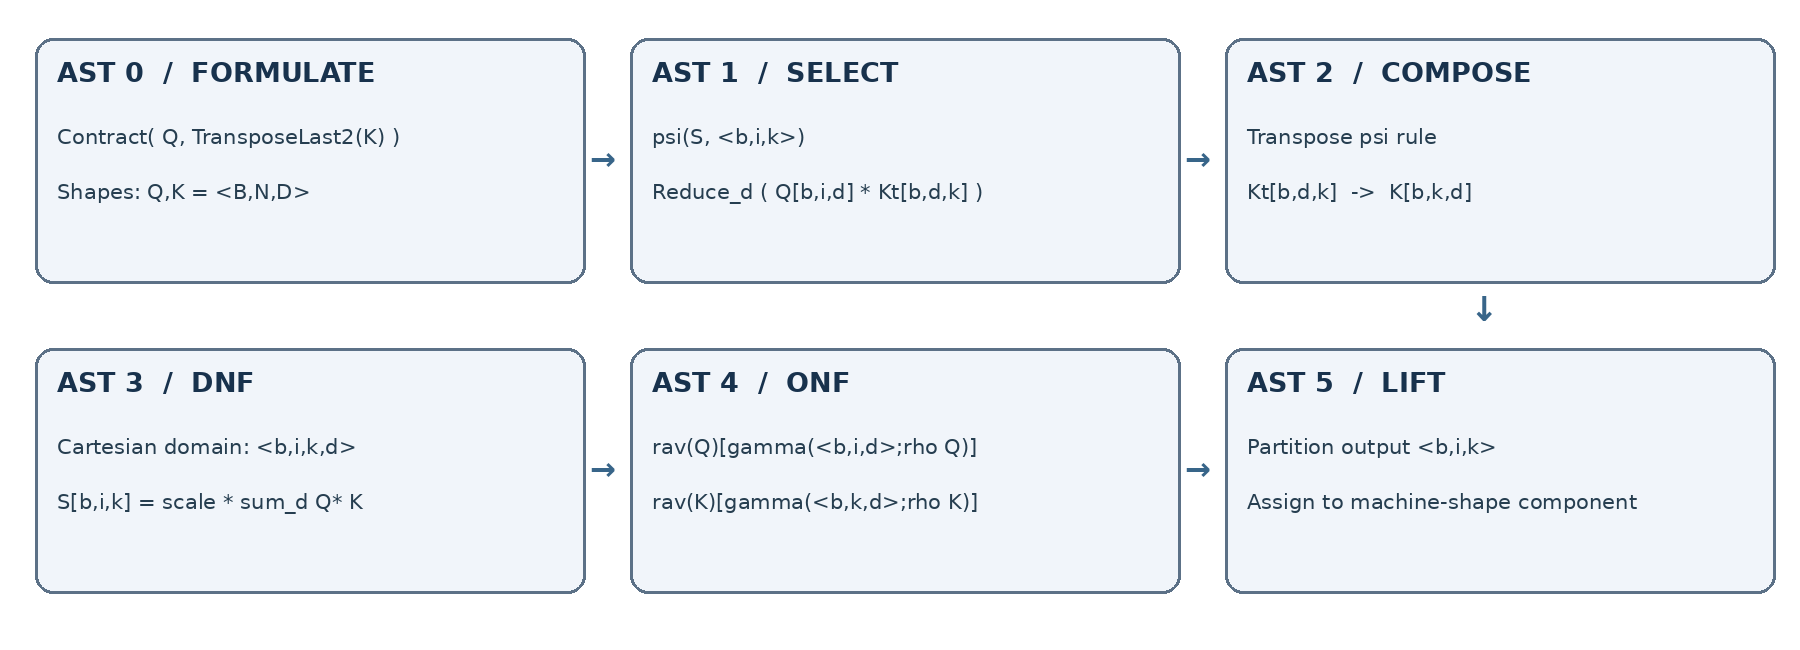
\includegraphics[width=.82\linewidth]{figure10_compact_ast_story.png}
\caption{Compact AST progression for one attention score component. Transpose-index composition converts the logical transpose into direct $K[b,k,d]$ selection; the resulting contiguous reduction is then addressed with the shape-dependent $\gamma$ family and assigned to machine-shape components. This is an illustrative AST trace, not compiler-generated output.}\label{fig:ast-chain-v7}
\end{figure}

\paragraph{AST 4 to AST 6: constructive machine instantiation.}
The sequential ONF replaces every selection with $\operatorname{rav}(X)[\gamma(\vec i;\rho X)]$. Dimension lifting assigns the Cartesian output domain to machine-shape components. For disjoint output ownership, define $f_c:[B]\times[N]\times[N]\to\iota(\rho\mathcal M_c)$, with $\mathcal D_m=f_c^{-1}(m)$. The proof obligation is $\bigcup_m\mathcal D_m=[B]\times[N]\times[N]$ with pairwise disjoint $\mathcal D_m$; if the reduction domain itself is partitioned, an additional explicit combination operation is required. The same DNF admits sequential, OpenMP, OpenACC, and MPI/Open MPI realizations, each lowering the same indexed computation according to the machine shape and its legal ownership and communication constraints.
\begin{figure}[htbp]\centering
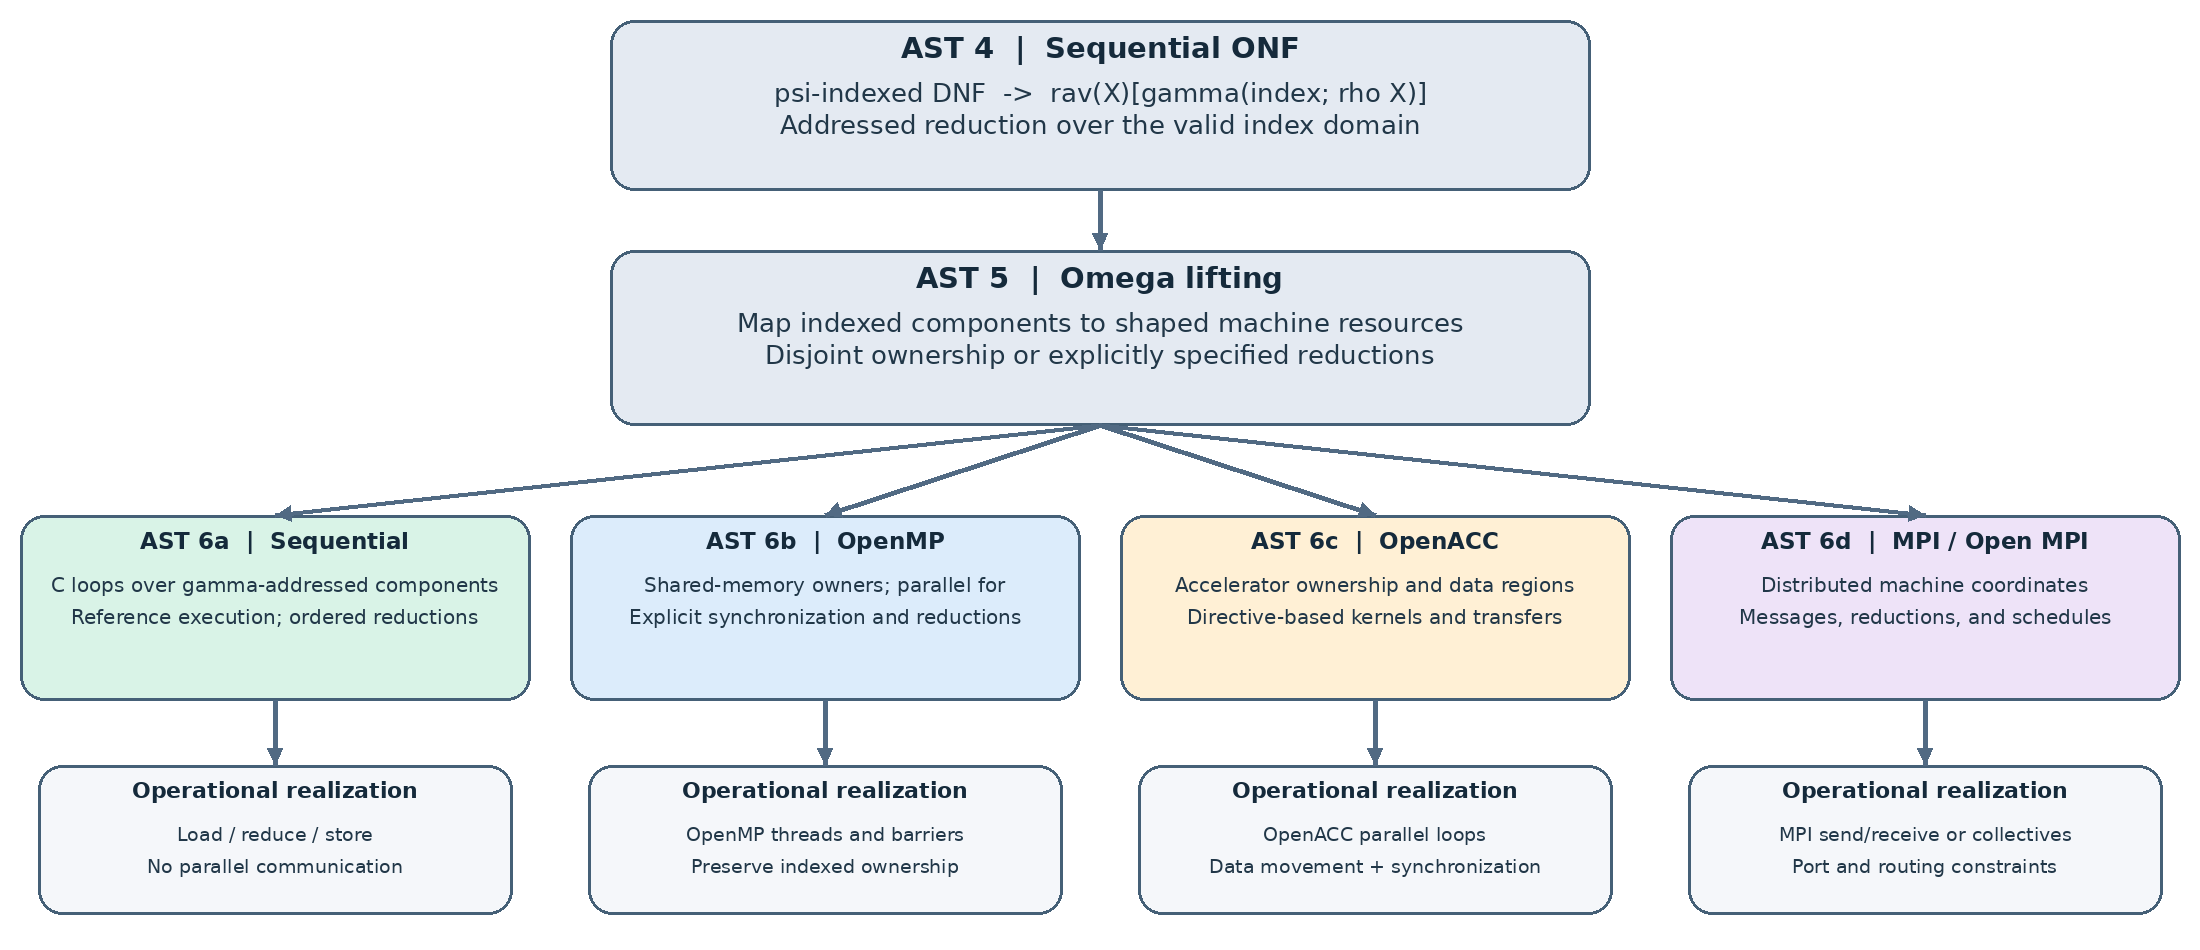
\includegraphics[width=.94\linewidth]{figure13_ast_to_instructions.png}
\caption{AST 4 $\to$ AST 5 $\to$ four realization branches: sequential, OpenMP, OpenACC, and MPI (with Open MPI as an implementation). All branches share the same Cartesian DNF and addressed ONF, with distinct ownership, transfer, reduction, and synchronization obligations. The diagram illustrates the portable target architecture, not four independently verified compiler emitters.}\label{fig:instructions-v7}
\end{figure}

\paragraph{Instruction-level correspondence.}
For a CPU-owned output component, the reduction body is instantiated as \texttt{load Q[gamma(<b,i,d>;rho Q)]}, \texttt{load K[gamma(<b,k,d>;rho K)]}, \texttt{multiply/add or fma}, followed by \texttt{store S[gamma(<b,i,k>;rho S)]}. A GPU-owned component uses corresponding device loads, arithmetic, and stores inside a kernel, with its block/thread index decoded into the lifted Cartesian index. A coordinated CPU--GPU realization additionally instantiates necessary copies or DMA transfers, stream or event dependencies, and a completion barrier. A device-specific backend must prove that these actual instructions implement the lifted ONF and respect its numerical contract; an FMA is not automatically bitwise equivalent to a separate multiply and add.

\paragraph{End-to-end attention.}
The same stepwise trace must subsequently be repeated for the maximum reduction, exponentiation, normalization, and the $P$--$V$ contraction, or for the corresponding fused online-softmax recurrence from Paper~1. These operations cannot be replaced by the score-only AST without losing dependencies. The figures establish the \emph{format of a checkable trace} and the explicit score-contraction example, not a claim that the full memory-optimal Paper~1 kernel has already been mechanically generated.


\section{AST-to-instruction evidence and the portable realization objective}
\label{sec:code-traces}
This section places code immediately after the AST sequence in Figures~\ref{fig:ast-chain-v7} and~\ref{fig:instructions-v7}. It instantiates the \emph{score contraction only}; the complete stable-softmax and value contraction of Paper~1 remain distinct derivations. Let $\rho Q=\rho K=\langle B,N,D\rangle$ and $\rho S=\langle B,N,N\rangle$. The shared Cartesian DNF is
\begin{equation}
\langle b,i,j\rangle\psi S = D^{-1/2}\sum_{d=0}^{D-1}
(\langle b,i,d\rangle\psi Q)(\langle b,j,d\rangle\psi K).
\end{equation}
AST~4 instantiates the row-major member of the $\gamma$ family:
$\gamma_{\rm row}(\langle a,b,c\rangle;\langle n_0,n_1,n_2\rangle)=(a n_1+b)n_2+c$.
The general definition remains $\vec i\psi X=(\operatorname{rav}X)[\gamma(\vec i;\rho X)]$; the code below is a specific row-major realization, not a restriction on MoA.

\subsection{AST~4: shape-dependent address instantiation}
\noindent\fbox{\parbox{.91\linewidth}{\footnotesize\textit{Source listing not bundled in the preserved v38 archive:} \texttt{attention\_cpu.c}, lines 9--12. This historical excerpt is intentionally not reconstructed or fabricated.}}
Here $\gamma(\langle b,i,d\rangle;\rho Q)$ and $\gamma(\langle b,j,d\rangle;\rho K)$ generate the two operand addresses. The logical last-two-dimension transpose of $K$ is eliminated by index composition; no physical transpose is allocated.

\subsection{AST~5a--6a: CPU ownership and C/OpenMP instructions}
\noindent\fbox{\parbox{.91\linewidth}{\footnotesize\textit{Source listing not bundled in the preserved v38 archive:} \texttt{attention\_cpu.c}, lines 15--32. This historical excerpt is intentionally not reconstructed or fabricated.}}
Each OpenMP iteration owns one element of the Cartesian output domain. The reduction $d$ is local to its owner, and all outputs are disjoint. The generated instruction classes are address calculation, load, multiply/add, scale, and store.

\subsection{AST~5b--6b: portable accelerator ownership with OpenACC}
The same lifted ONF assigns each output component to one owner. The following is a \emph{schematic OpenACC realization} of the score contraction, not evidence of a separately tested compiler emitter:
\begin{lstlisting}[language=C]
#pragma acc parallel loop collapse(3) present(Q[0:B*N*D],K[0:B*N*D],S[0:B*N*N])
for (size_t b=0; b<B; ++b)
 for (size_t i=0; i<N; ++i)
  for (size_t j=0; j<N; ++j) {
   float acc=0.0f;
   for (size_t d=0; d<D; ++d)
    acc += Q[(b*N+i)*D+d]*K[(b*N+j)*D+d];
   S[(b*N+i)*N+j]=acc/sqrtf((float)D);
  }
\end{lstlisting}
The OpenACC data region and execution configuration are realization obligations; the $\gamma$ addresses and output ownership are derived from MoA. The displayed code is illustrative and requires compiler, numerical, and runtime validation.

\subsection{AST~5c--6c: sequential, OpenMP, OpenACC, and MPI realizations}
The sequential ONF is the reference execution. OpenMP assigns disjoint output indices to shared-memory workers; OpenACC assigns them to accelerator workers; MPI partitions the same index domain among processes (with Open MPI as one MPI implementation). For a distributed partition $\mathcal D_r$, each process computes only its owned outputs, with required input transfers and any necessary reductions determined by the $\psi$ dependencies. A coordinated OpenMP--OpenACC--MPI execution is a \emph{target architecture}, not an assertion that the current prototype has already generated and validated all four paths. Figure~\ref{fig:instructions-v7} illustrates the intended lowering.

\section{Proof obligations and compiler acceptance criteria}
A complete mechanization must exhibit a verifiable sequence: (1) shape-correct AST construction; (2) $\psi$-reduction and DNF semantic preservation; (3) layout-specific $\gamma$ mapping to sequential ONF; (4) dimension-lifted disjoint coverage and dependency preservation; (5) valid mapping to resource capacities and communication topology; (6) code generation whose numerical semantics match the reference contract; and (7) pre-execution resource, time, and energy predictions assessed against independent hardware measurements. This is a research agenda, not a claim that all obligations have already been discharged by the current prototype.


\section{Complete forward attention: DNF to memory-reduced lifted ONF}
\label{sec:full-forward}
The previous contraction is only the first part of forward attention. Here we trace the stable normalization and the subsequent value contraction to executable code. This section distinguishes (i) the reference, hand-derived Paper~1 forward equations and their tiled implementation from (ii) the \emph{online-summary realization} developed here as a candidate compiler rewrite. The latter is not attributed to Paper~1's original C implementation. Its correspondence to DNF is established algebraically and checked numerically below.

\subsection{AST A: the full mathematical specification}
For $\rho Q=\langle n,d\rangle$, $\rho K=\langle m,d\rangle$, $\rho V=\langle m,d_v\rangle$, the result has shape $\rho O=\langle n,d_v\rangle$. The score uses MoA MM with the logical transpose of the last two dimensions of $K$:
\begin{align}
 s_{ik}&=d^{-1/2}\sum_{j=0}^{d-1}(\langle i,j\rangle\psi Q)(\langle k,j\rangle\psi K),\\
 a_i&=\max_{0\le k<m}s_{ik},\qquad
 z_i=\sum_{k=0}^{m-1}\exp(s_{ik}-a_i),\\
 \langle i,v\rangle\psi O&=z_i^{-1}\sum_{k=0}^{m-1}\exp(s_{ik}-a_i)(\langle k,v\rangle\psi V).
 \label{eq:full-dnf}
\end{align}
Figure~\ref{fig:fullast} places the AST rewrite stages alongside their defining formulas. The Cartesian domain $\{(i,k,j,v)\}$ is finite and shape-bounded. The final $k$-reduction is the MoA value contraction; neither a score matrix nor a probability matrix is required by its denotation.
\begin{figure}[htbp]\centering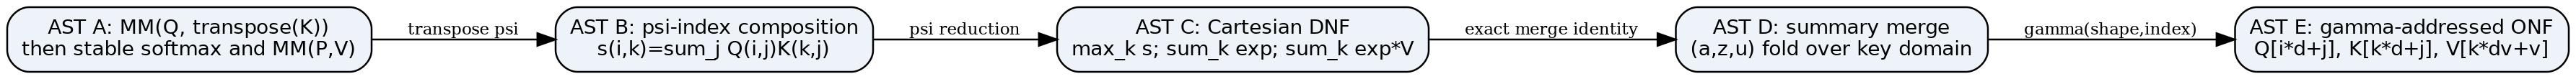
\includegraphics[width=.90\linewidth]{full_forward_ast.png}\caption{Traceable full-forward attention ASTs: the score MM transpose-index rewrite, stable normalization, value contraction, stable summary, and addressed/lifted ONF. Each arrow has an explicit equation in the text.}\label{fig:fullast}\end{figure}

\subsection{AST B: stable normalization as a mergeable MoA reduction}
For any nonempty key-index subset $H\subseteq\{0,\ldots,m-1\}$, define the summary
\begin{equation}
 F_i(H)=(a_H,z_H,\vec u_H),\quad
 a_H=\max_{k\in H}s_{ik},\quad z_H=\sum_{k\in H}e^{s_{ik}-a_H},\quad
 \langle v\rangle\psi\vec u_H=\sum_{k\in H}e^{s_{ik}-a_H}(\langle k,v\rangle\psi V).
\end{equation}
For disjoint $H_1,H_2$, write $F_i(H_1)\oplus F_i(H_2)=(a,z,\vec u)$, where
\begin{align}
 a&=\max(a_1,a_2),\\
 z&=e^{a_1-a}z_1+e^{a_2-a}z_2,\\
 \langle v\rangle\psi\vec u&=e^{a_1-a}(\langle v\rangle\psi\vec u_1)+e^{a_2-a}(\langle v\rangle\psi\vec u_2).
 \label{eq:merge-full}
\end{align}
Substitution shows that the merged $a$ is the maximum on $H_1\cup H_2$ and that $z,\vec u$ are precisely the sums normalized by this common maximum. Thus the merged summary is equal to $F_i(H_1\cup H_2)$ in exact arithmetic. The empty set has identity $(a,z,\vec u)=(-\infty,0,\vec 0)$ with the usual guarded update. This establishes a constructive rewrite from the DNF reductions to a fold over $k$ and permits any disjoint partition of the key domain. For floating-point execution, different merge orders may round differently.

\subsection{AST C: memory-reduced online ONF}
For the ordered key domain $k=0,\ldots,m-1$, the sequential fold updates $(a,z,\vec u)$ by merging its current summary with the singleton summary $(s_{ik},1,\langle k,\cdot\rangle\psi V)$. Its final output is
\begin{equation}
 \langle i,v\rangle\psi O=(\langle v\rangle\psi\vec u)/z.
\end{equation}
This realization requires $O(d_v)$ scratch per active query and does not materialize the $n\times m$ score or probability arrays. The original Paper~1 reference C code supplied in the source comparison uses a row scratch array and tiled score operations; the online-summary fold here is a separate, mathematically derived optimization candidate. Neither construction implies zero communication on a key-sharded distributed machine.

\subsection{AST D: shape-dependent addresses and instruction lowering}
For row-major $Q,K,V,O$, the selections become
\begin{align}
 \langle i,j\rangle\psi Q&=(\operatorname{rav}Q)[\gamma_{\rm row}(\langle i,j\rangle;\rho Q)],\\
 \langle k,j\rangle\psi K&=(\operatorname{rav}K)[\gamma_{\rm row}(\langle k,j\rangle;\rho K)],\\
 \langle k,v\rangle\psi V&=(\operatorname{rav}V)[\gamma_{\rm row}(\langle k,v\rangle;\rho V)].
\end{align}
The corresponding C expressions are \texttt{Q[i*d+j]}, \texttt{K[k*d+j]}, and \texttt{V[k*dv+v]}. The inner $j$ traversals of $Q,K$ are contiguous; $V[k*dv+v]$ traverses the $v$ dimension contiguously for each key. Other $\gamma$ families yield different regular address sequences, potentially using strided DMA.
\begin{figure}[htbp]\centering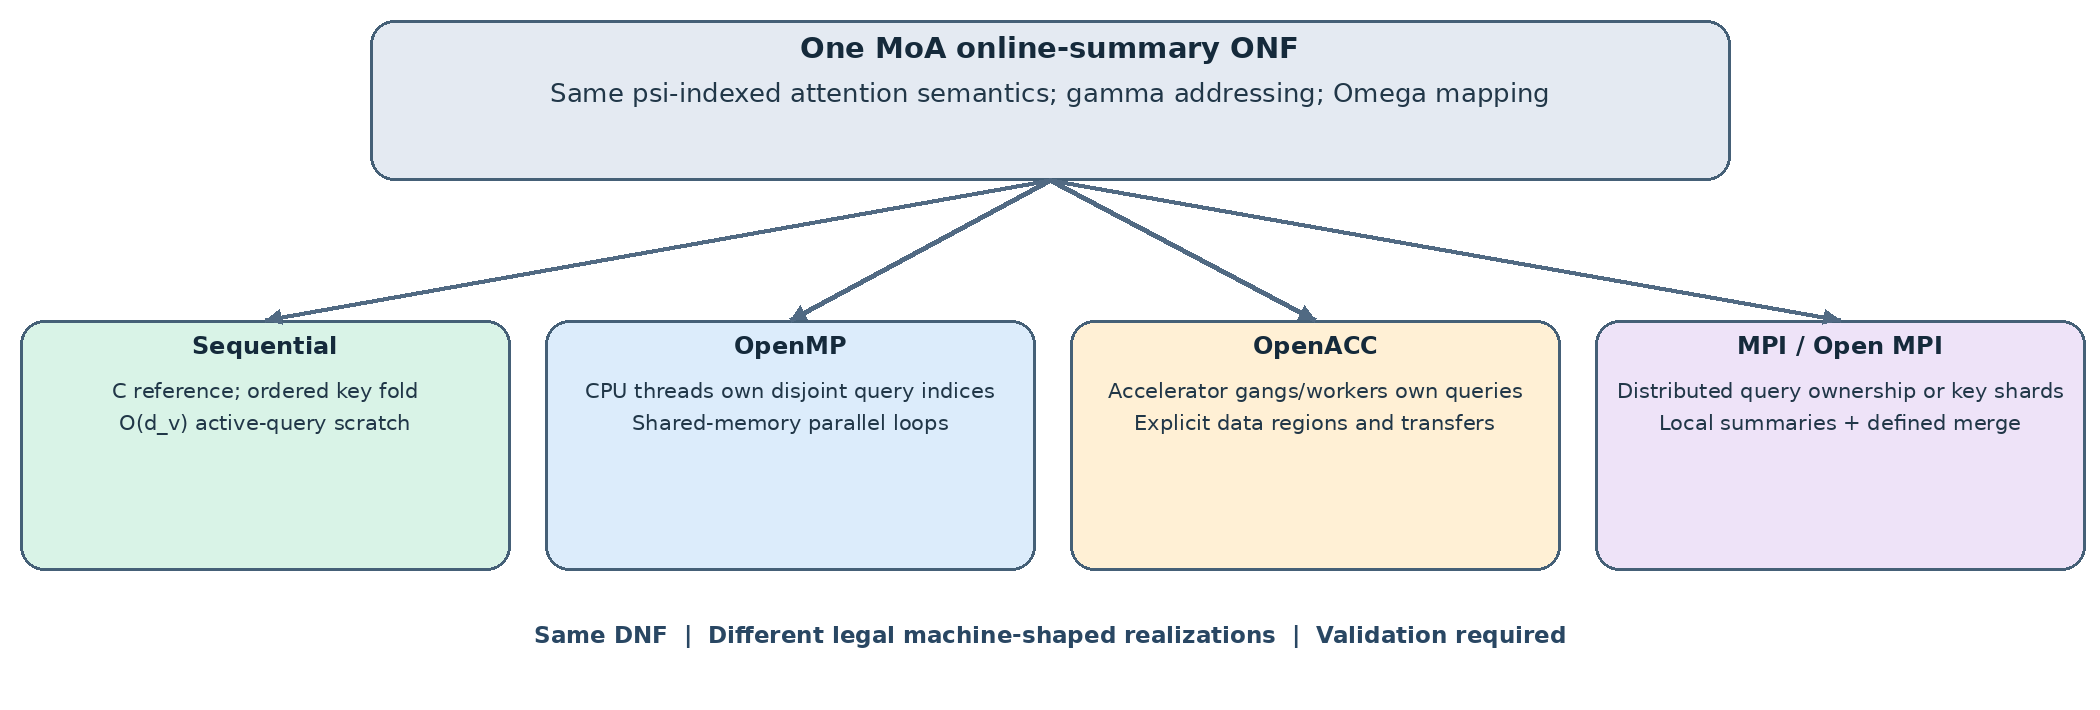
\includegraphics[width=.94\linewidth]{full_forward_lowering.png}\caption{One online-summary ONF and four intended realizations: sequential C, shared-memory OpenMP, accelerator OpenACC, and distributed MPI/Open MPI. A key-sharded distributed mapping merges local $(a,z,\vec u)$ summaries using Eq.~\eqref{eq:merge-full}. The figure shows the target design rather than verified generation of every backend.}\label{fig:fullcode}\end{figure}

\subsection{AST E: CPU, GPU, and coordinated heterogeneous realization}
The companion source \texttt{attention\_full\_cpu.c} contains both the DNF reference and a C/OpenMP online-summary realization. The full forward path is shown here, not just the score contraction:
\noindent\fbox{\parbox{.91\linewidth}{\footnotesize\textit{Source listing not bundled in the preserved v38 archive:} \texttt{attention\_full\_cpu.c}, lines 37--57. This historical excerpt is intentionally not reconstructed or fabricated.}}
The CUDA C example \texttt{attention\_full\_gpu.cu} maps one query index to each GPU thread and implements the same summary recurrence. Its demonstrator-local $d_v$ bound is an implementation constraint, not an MoA restriction. A heterogeneous mapping partitions the query index set into disjoint CPU and GPU subsets, transfers the necessary $K,V$ data, launches the GPU subset, and combines the disjoint output regions. The companion CUDA source includes the GPU kernel and a launch fragment. It is \emph{illustrative and not yet validated on a CUDA device}; a production realization must include transfer, synchronization, error handling, and machine-dependent scheduling.

\subsection{Validation and compiler acceptance gate}
For $n=7,m=11,d=9,d_v=5$ and deterministic inputs, the CPU DNF reference and OpenMP online realization were compiled with GCC and compared: maximum absolute output difference $1.11\times10^{-16}$. This is a small numerical smoke test, not a general proof of IEEE floating-point equivalence or GPU correctness. The mathematical summary identity supplies the exact-arithmetic equivalence argument. The compiler acceptance gate is an emitted AST rewrite trace, proof of partition coverage, shape-correct $\gamma$ addresses, a faithful target lowering, and numerical tests over varying shapes, layouts, and target resources. Time and energy optimality remain empirical and predictive research objectives.


\section{A reproducible AST-to-C mechanization prototype}
\label{sec:generated}
The previous code examples were hand-written realizations. This section adds a \emph{small executable code-generation prototype} rather than claiming that a general MoA compiler is complete. The companion script \texttt{moa\_ast\_codegen.py} records five structured AST stages (A--E) as \texttt{ast\_rewrite\_trace.json}, emits \texttt{generated\_attention\_cpu.c}, and checks bounded index properties. The AST stages are: (A) attention specification, (B) $\psi$-reduced DNF, (C) stable $(a,z,\vec u)$ summary fold, (D) shape-dependent $\gamma$ addressing, and (E) query-domain ownership under $\Omega$ lifting. The source-to-source generator is presently a restricted, template-based lowering of this single derived operation; it does not yet parse arbitrary Fortran, MATLAB, Python, or Julia expressions.

\begin{figure}[htbp]\centering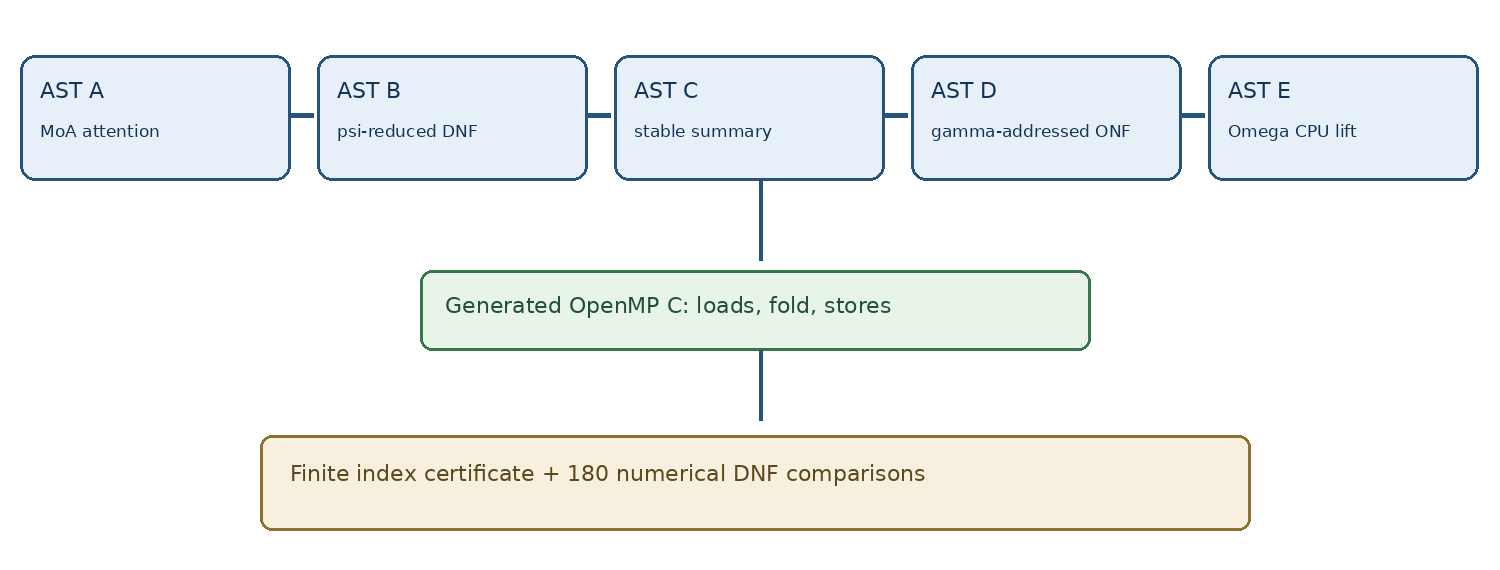
\includegraphics[width=.91\linewidth]{generated_ast_proof_chain.png}\caption{Executable prototype trace: each named MoA AST stage precedes CPU code emission. The bounded certificate verifies address and ownership properties on sampled finite shape domains; the exact-arithmetic summary identity is established separately in Eq.~\eqref{eq:merge-full}.}\label{fig:genchain}\end{figure}

\paragraph{Index and ownership certificate.}
For row-major arrays, $\gamma_{\rm row}(\langle i,j\rangle;\langle r,c\rangle)=ic+j$ on $0\le i<r$, $0\le j<c$. The generator enumerates 288 finite combinations of positive $n,m,d,d_v$ and worker counts, checking that this $\gamma$ is a bijection onto $[0,rc)$ for each relevant array shape and that the lifted ownership rule $i=w+tp$ ($0\le w<p$, $t\ge0$, $i<n$) assigns every query index exactly once. These exhaustive checks \emph{within the declared finite domain} are reproducible evidence, not a proof for all natural-number shapes. For arbitrary positive $p$, uniqueness follows because $i\bmod p$ identifies the unique owner $w$, and completeness follows by Euclidean division $i=p\lfloor i/p\rfloor+(i\bmod p)$.

\paragraph{Generated instructions and test.}
The generated C uses the indexed contraction $Q[\gamma(\langle i,j\rangle;\rho Q)]K[\gamma(\langle k,j\rangle;\rho K)]$, then the stable summary recurrence, with one OpenMP-owned output row per $i$. The emitted kernel is in \texttt{generated\_attention\_cpu.c}; \texttt{test\_generated.c} compares it to a separately coded materialized-score DNF reference. With GCC \texttt{-O2 -fopenmp}, 180 positive-shape cases passed; the maximum observed absolute difference was $4.44\times10^{-16}$. This supports a limited numerical regression claim, not bitwise equivalence or formal verification of generated instructions.

\paragraph{Target scope and next proof gates.}
The CUDA and CPU--GPU paths were subsequently compiled and exercised on UAlbany DGX hardware, as documented in Section~\ref{sec:v13hardware}; this does not establish arbitrary-shape correctness or an optimal scheduler. To reach the universal objective, the generator must accept general MoA ASTs, implement verified rewrite rules rather than fixed templates, emit per-step certificates, and lower the same lifted ONF into CPU, GPU, and coordinated CPU--GPU instruction sequences with validated transfer and synchronization behavior. Performance, power, and energy predictions remain separate empirical obligations.


\section{Restricted rewrite passes and three executable target lowerings (v12)}
\label{sec:threebackends}
We extend the earlier fixed CPU template with an explicit sequence of \emph{typed, restricted} AST passes, implemented in \texttt{moa\_rules\_v12.py}. The input is a forward-attention node with shapes $\rho Q=\langle n,d\rangle$, $\rho K=\langle m,d\rangle$, $\rho V=\langle m,d_v\rangle$, and $\rho O=\langle n,d_v\rangle$. The passes are not a general parser or a formal proof assistant. Their observable intermediate nodes are recorded in \texttt{ast\_rule\_trace\_v12.json}:
\begin{equation}
\underbrace{\operatorname{MM}(Q,K^{T_{\mathrm{last}\,2}})}_{\mathrm{AST}_0}
\xrightarrow{\psi\text{-composition}}
\underbrace{\sum_j (\langle i,j\rangle\psi Q)(\langle k,j\rangle\psi K)}_{\mathrm{AST}_1}
\xrightarrow{\text{stable summary}}
\underbrace{(a,z,\vec u)}_{\mathrm{AST}_2}
\xrightarrow{\gamma(\vec\imath;\rho X)}
\mathrm{AST}_3
\xrightarrow{\Omega_{\mathcal M}}\mathrm{AST}_4.
\end{equation}
The first AST arrow is the mathematical transpose-index composition; the second is the exact-arithmetic summary identity in Eq.~\eqref{eq:merge-full}. The addressing pass uses the shape of \emph{each selected array}, rather than a shape-free offset. The final ownership pass is parameterized by CPU, GPU, or coordinated CPU--GPU target.

\paragraph{CPU instantiation.} The generated \texttt{generated\_v12\_cpu.c} implements the stable summary using OpenMP query ownership and the shape-derived row-major $\gamma$ address family. Each query index is assigned once, and the $j$-reduction visits contiguous components of the original $Q$ and $K$. The separate materialized-score DNF reference and the generated CPU realization were compared across 180 positive-shape cases, with a maximum absolute difference of $4.44\times10^{-16}$ in the recorded v12 regression. This is numerical evidence, not a proof of identical IEEE floating-point evaluation.

\paragraph{GPU instantiation.} The generated \texttt{generated\_v12\_gpu.cu} maps query indices to CUDA block/thread coordinates. The same $\gamma$ operands and stable summary recurrence appear inside each thread. The demonstrator uses per-thread local scratch of at most 64 value components; this is an implementation bound, not an MoA restriction. Subsequent UAlbany DGX compilation and numerical testing are reported in Section~\ref{sec:v13hardware}.

\paragraph{Coordinated CPU--GPU instantiation.} The generated \texttt{generated\_v12\_cpu\_gpu.cu} partitions the query domain into $[0,s)$ for CPU and $[s,n)$ for GPU. It includes device allocation, input transfers, a GPU launch, concurrent host computation, synchronization, transfer of the GPU-owned output range, and cleanup. The sets are disjoint and cover $[0,n)$, but optimal $s$ is not yet predicted. In particular, this host coordinator is generated as a target-specific wrapper around the shared lifted operation, not as a proved optimal heterogeneous scheduler.

\paragraph{Evidence and limitations.} The current construction demonstrates reusable named transformation passes and three backend code emitters for a \emph{restricted attention operation}. The AST trace is inspectable, but no independent machine-checkable proof certificates have been produced. The restricted CPU, CUDA, and coordinated CPU--GPU paths have now been compiled and numerically exercised on DGX hardware (Section~\ref{sec:v13hardware}); generality, formal proof certificates, and predictive timing remain open. General source-language front ends, multiple layouts, cross-device summary reductions, and prediction of time and energy from deterministic machine shapes remain future compiler milestones.


\section{DGX hardware validation of generated CPU--GPU attention (v13)}
\label{sec:v13hardware}
\paragraph{Provenance and claim boundary.} This section reports an additional October 30, 2026 experimental session on University at Albany DGX nodes, distinct from the earlier calibration/holdout study. The restricted v12 code generator emitted the CPU, CUDA, and coordinated host wrapper. The source and measurement transcript supplied for this update establish execution and finite numerical tests; they do not establish a proof of unrestricted machine-shape correctness, optimal splitting, or a calibrated time/energy predictor. Prior attention studies were hand-derived and implemented, not produced by this compiler.

\subsection{MoA output ownership and execution realization}
For the tested forward-attention output with $\rho O=\langle n,d_v\rangle$, the CPU--GPU split $s$ assigns query-index sets
\begin{equation}
I_{\rm CPU}=\{i\mid 0\le i<s\},\quad I_{\rm GPU}=\{i\mid s\le i<n\},\quad I_{\rm CPU}\mathbin{\dot\cup}I_{\rm GPU}=\{0,\ldots,n-1\}.
\end{equation}
Each output $\langle i,v\rangle\psi O$ is owned exactly once. The tested coordinator allocates device buffers, transfers $Q,K,V$, launches GPU work for $I_{\rm GPU}$, executes the CPU-owned $\psi$-indexed work, synchronizes, transfers GPU-owned output components, and releases device buffers. The index-to-address realization uses $\gamma$ on the original shaped arrays; the split changes ownership, not the DNF.
\begin{figure}[htbp]\centering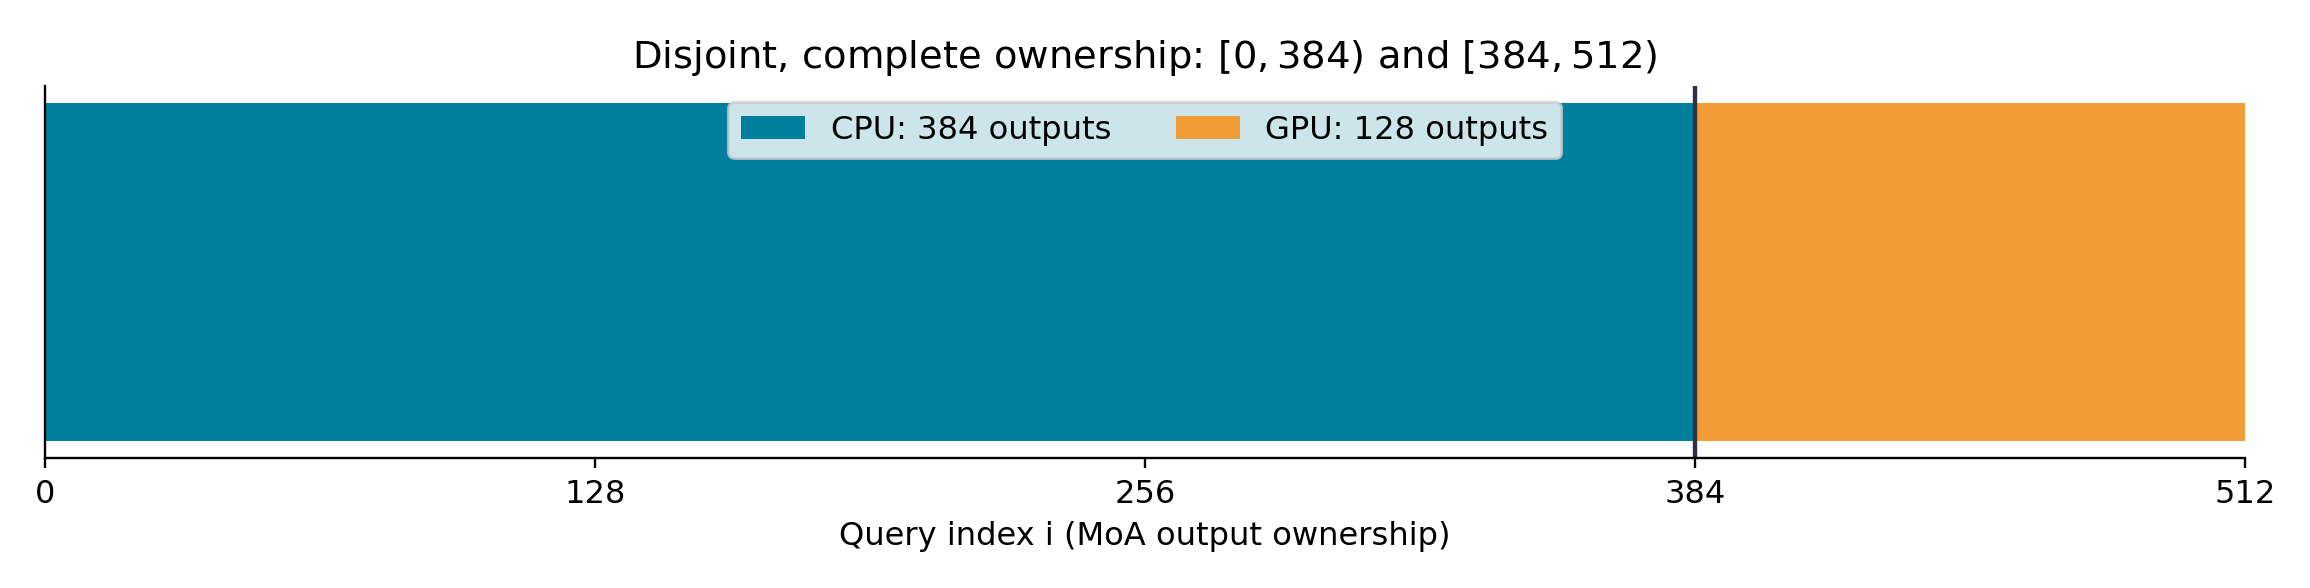
\includegraphics[width=.95\linewidth]{v13_ownership.png}\caption{Color-coded, complete ownership for $n=512$, $s=384$. The CPU owns $75\%$ of query indices; the GPU owns the remaining $25\%$.}\label{fig:v13ownership}\end{figure}

\subsection{Experimental configuration and numerical checks}
The measured attention shape was $n=m=512$, $d=d_v=64$, with four OpenMP threads bound to cores $0,1,64,65$ on DGX12, an AMD EPYC 7742 node with an NVIDIA A100-SXM4-80GB GPU. The diagnostic used one untimed warmup and ten timed wrapper invocations, with \texttt{CLOCK\_MONOTONIC} timing. CUDA 12.8 and Nsight Systems 2024.6.2 were used for kernel and runtime profiling. The CPU ownership split was $s=384$; the GPU processed 128 query indices. A checksum of $125.183536304$ was reproduced by the phase-instrumented benchmark.

The reported regression sessions also tested five ownership splits (GPU-only, CPU-25\%, CPU-50\%, CPU-75\%, and CPU-only) on 36 larger shapes each, with observed maximum absolute numerical differences no larger than $1.84\times10^{-16}$ in those runs. Earlier tests covered 180 shape cases per mapping. These are finite numerical comparisons, not a proof of bitwise-identical floating-point results for all shapes.

\subsection{Kernel stability versus host-wrapper variability}
Nsight Systems recorded 11 executions of \texttt{moa\_gpu\_rows}, including warmup: mean $6.707529$ ms, median $6.707384$ ms, minimum $6.703128$ ms, maximum $6.710808$ ms. The full range was only $7.680$ microseconds. GPU launch-to-execution delays were typically $13$--$14$ microseconds. Figure~\ref{fig:v13kernel} displays each kernel duration.
\begin{figure}[htbp]\centering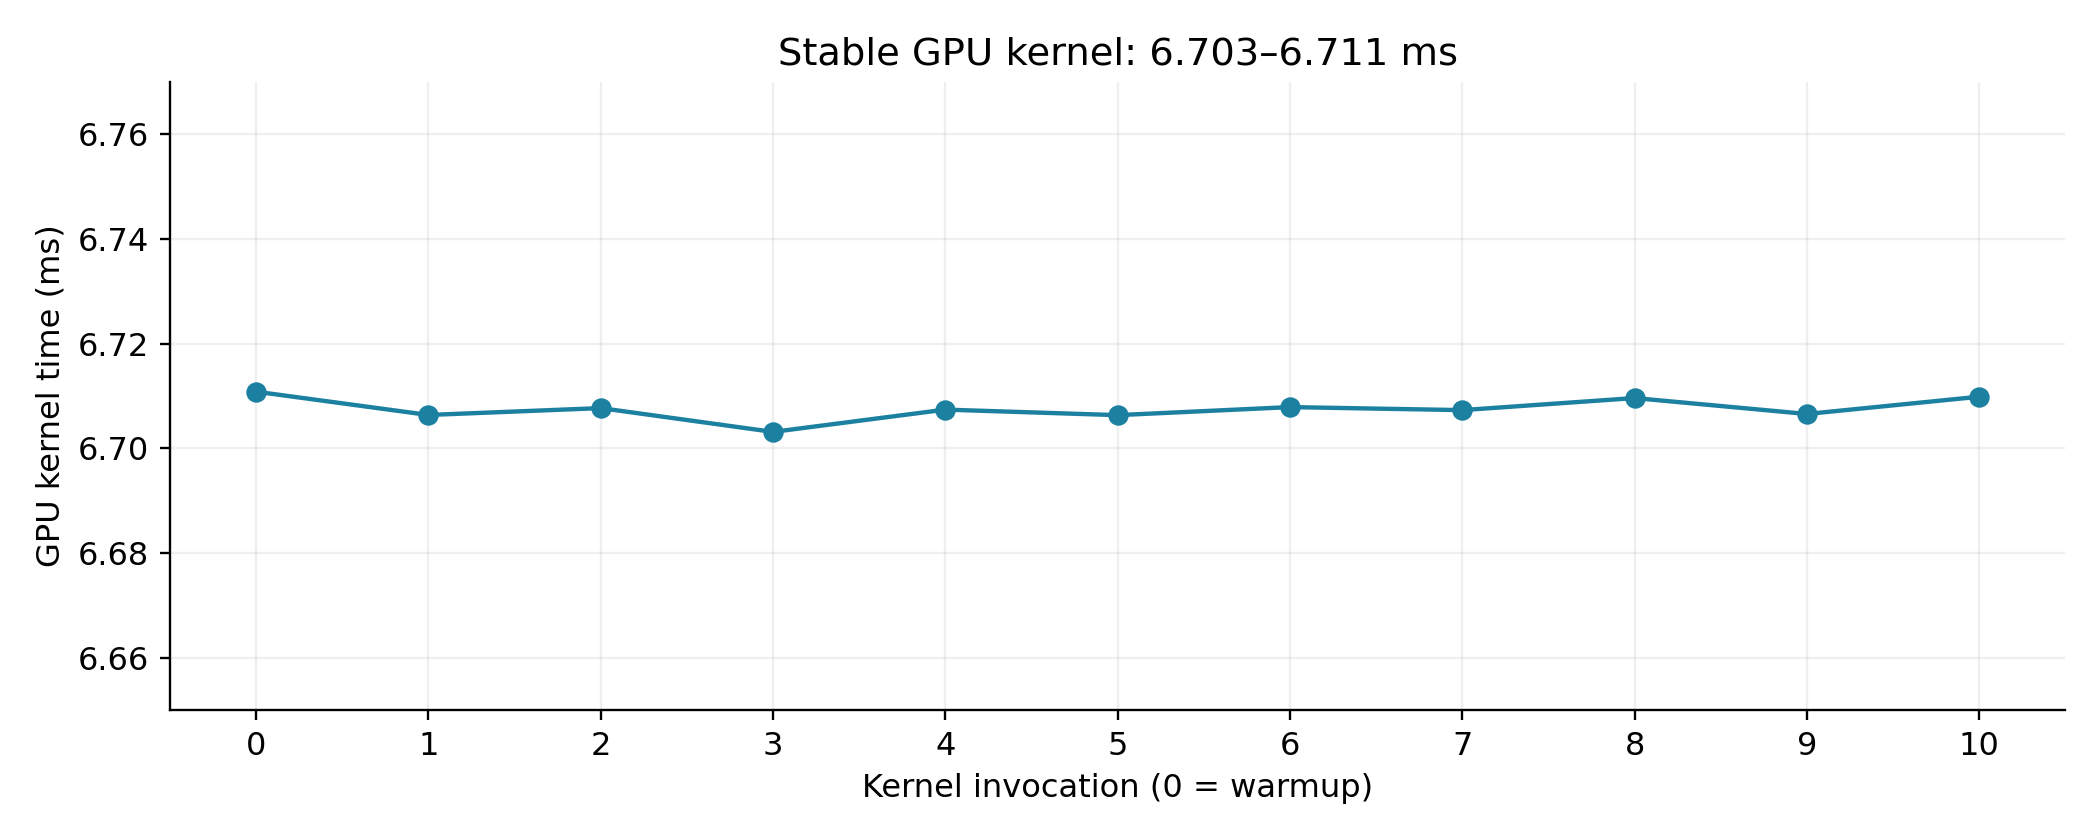
\includegraphics[width=.88\linewidth]{v13_kernel_stability.png}\caption{GPU kernel timing on DGX12 for the CPU-75\% mapping. The GPU computation was stable despite variability in the complete host wrapper.}\label{fig:v13kernel}\end{figure}

For the same mapping, the phase-instrumented benchmark recorded ten wrapper invocations with mean $7.473673$ ms, minimum $7.270481$ ms, and maximum $8.601487$ ms. The measured CPU-owned range typically took about $5.53$ ms (timed range $5.513719$--$5.707848$ ms). The CPU and GPU durations overlap and must \emph{not} be added to predict total elapsed time. Figure~\ref{fig:v13summary} compares the independently observed quantities without implying additivity.
\begin{figure}[htbp]\centering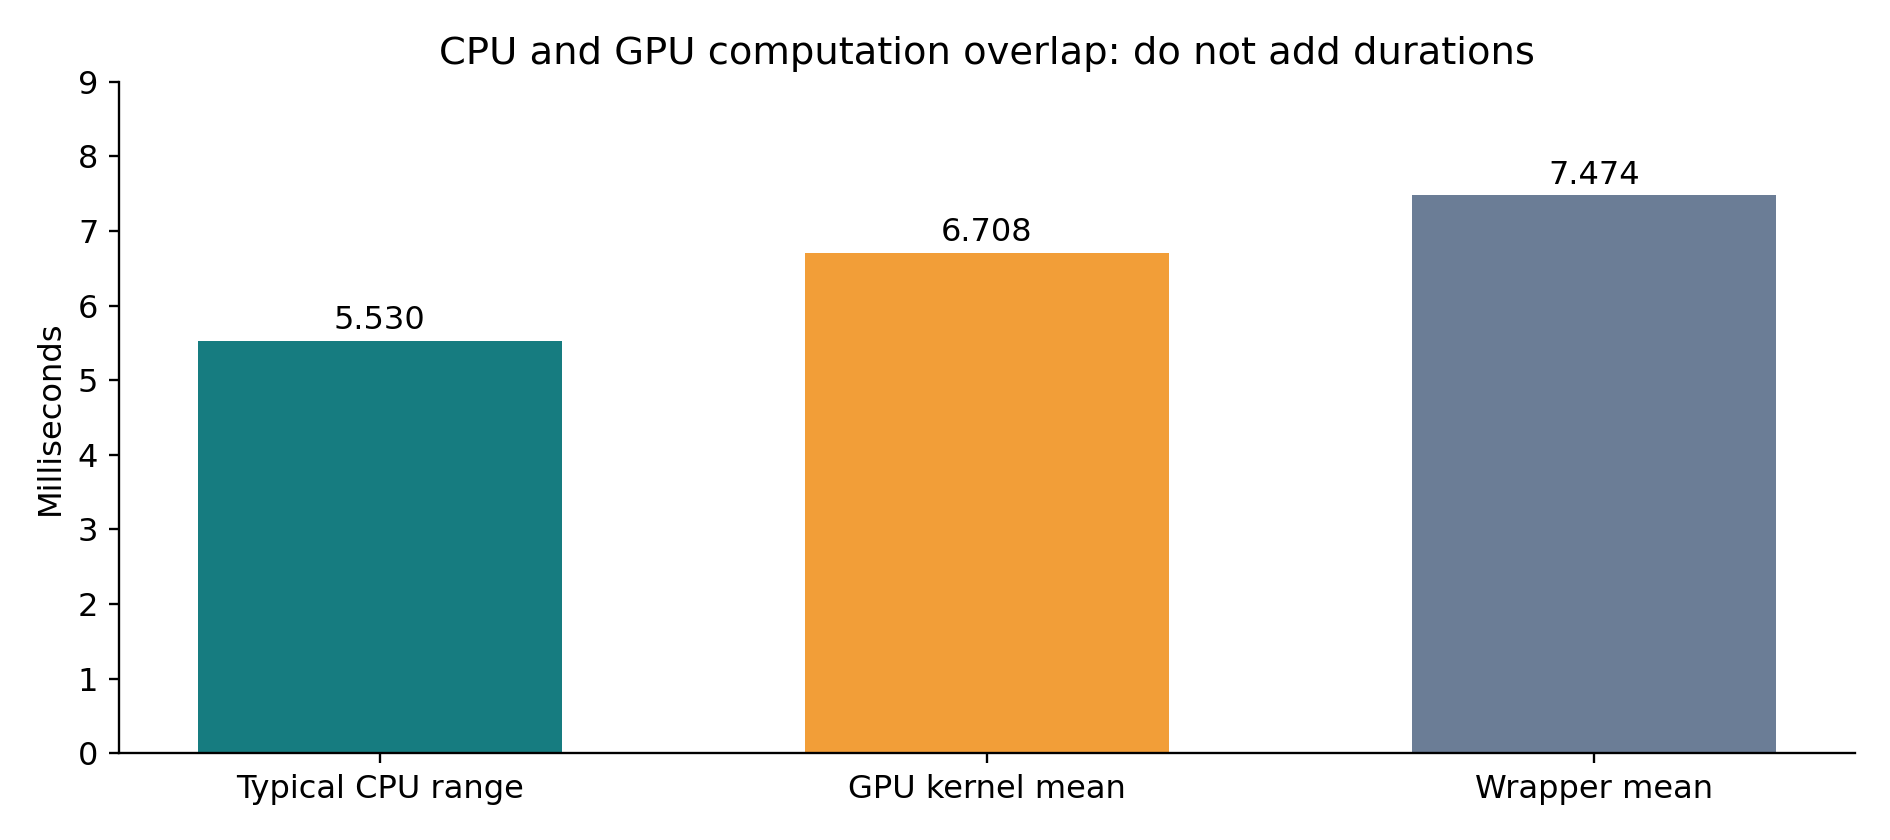
\includegraphics[width=.80\linewidth]{v13_execution_summary.png}\caption{CPU-owned computation, GPU kernel, and end-to-end wrapper times are different measurements. CPU and GPU work execute concurrently.}\label{fig:v13summary}\end{figure}

\subsection{Measured phase costs and outliers}
The wrapper was instrumented around CUDA allocation, host-to-device transfers, the CPU-owned work, device synchronization, device-to-host output transfer, and buffer cleanup. The measured phase costs are \emph{host-side elapsed intervals}; CUDA synchronization is a wait for outstanding GPU work, not an independent GPU computation cost. The GPU launch and small bookkeeping costs are included in the total but not represented as a separate stacked phase in Figure~\ref{fig:v13phases}.
\begin{table}[htbp]\centering\small
\caption{Representative phase durations in the ten timed DGX12 CPU-75\% invocations. Values are approximate typical durations, except where identified as observed outliers.}\label{tab:v13phases}
\begin{tabular}{lll}\toprule Phase & Typical time (ms) & Observed variation \\\midrule
CUDA allocation & 0.21 & 1.536 in repeat 6 \\
Host-to-device transfer & 0.105 & relatively stable \\
CPU-owned computation & 5.53 & 5.514--5.708 \\
CUDA synchronization & 1.20 & 1.031--1.218 \\
Device-to-host output transfer & 0.022 & relatively stable \\
CUDA cleanup & 0.19--0.20 & 0.685 in repeat 5 \\\bottomrule\end{tabular}
\end{table}
\begin{figure}[htbp]\centering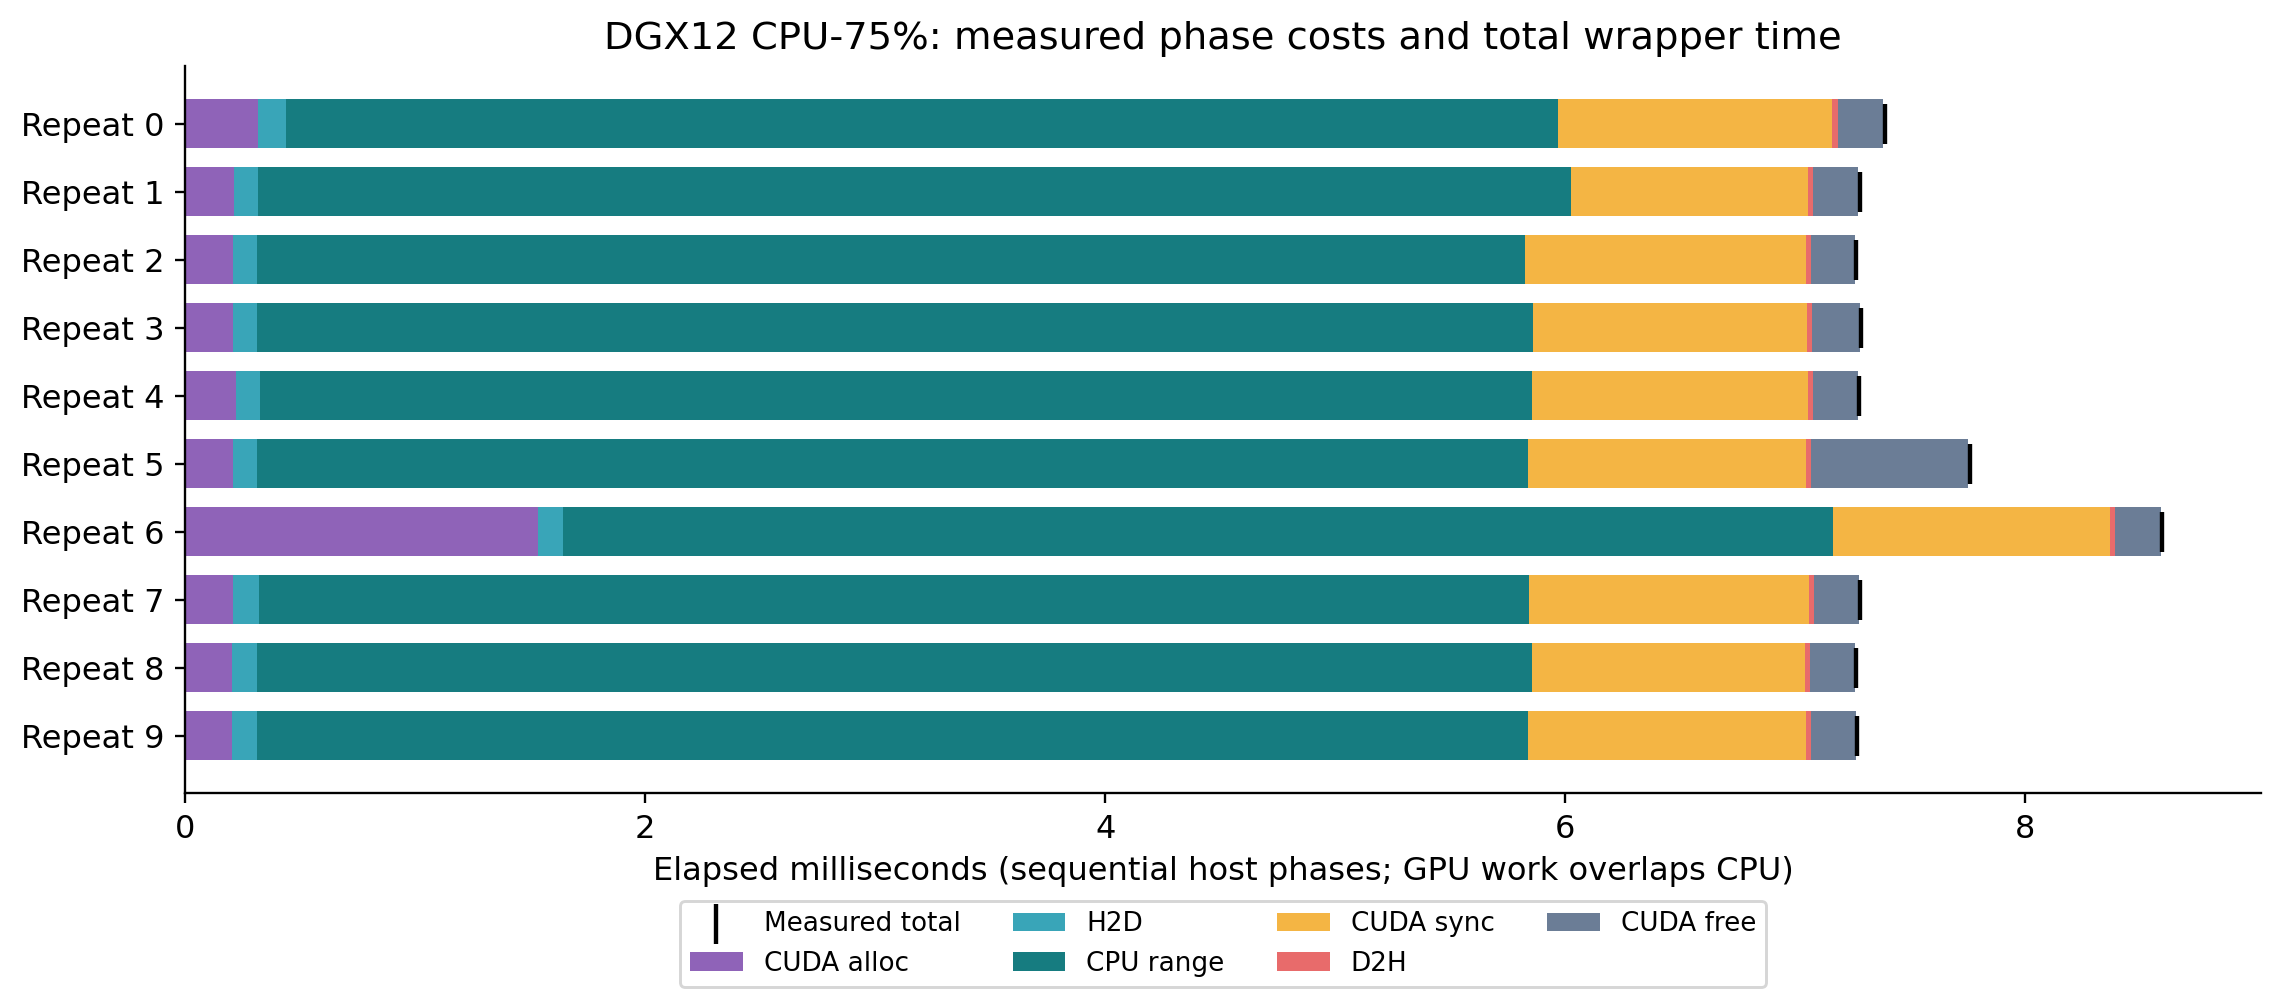
\includegraphics[width=.98\linewidth]{v13_phase_timing.png}\caption{Color-coded measured host phase intervals across ten timed invocations; black ticks mark total wrapper times. Phase sums omit small launch/bookkeeping intervals. Repeat 5 exhibits longer cleanup; repeat 6 exhibits longer allocation. GPU kernel execution overlaps CPU work.}\label{fig:v13phases}\end{figure}

Repeat 5 took $7.765451$ ms, with cleanup measured at $0.684628$ ms. Repeat 6 took $8.601487$ ms, with allocation measured at $1.536014$ ms. The untimed warmup took $434.711314$ ms in this phase-instrumented run, including $342.016789$ ms in the allocation phase; warmup was excluded from the reported mean. A separate Nsight trace recorded a $194.855754$ ms first allocation, also during warmup. Different startup measurements must not be conflated.

In the Nsight trace, one invocation entered \texttt{cudaDeviceSynchronize} approximately $1.265$ ms \emph{after} the GPU kernel had finished, producing a roughly $0.005$ ms synchronization call. The generated source calls \texttt{moa\_cpu\_range} before synchronization, so this indicates delayed host progress on that invocation, but does not isolate arithmetic from OpenMP scheduling or other host overhead. An earlier timed invocation of approximately $408$ ms was observed in another run; its cause was not established and it was not reproduced in the final phase-level experiment.

\subsection{Implications for machine-shape prediction}
The finite numerical tests support the correctness of the tested $\Omega$-lifted ownership realization. The GPU kernel timings show a stable computation component. The host wrapper, however, includes allocation, data movement, scheduling, synchronization, and cleanup that can vary independently of the mathematical index partition. A useful end-to-end model must describe the temporal overlap and the runtime phases without double counting:
\begin{equation}
T_{\rm wrapper}=T_{\rm allocation}+T_{\rm H2D}+T_{\rm launch/host}+T_{\rm overlap\;interval}+T_{\rm D2H}+T_{\rm cleanup},
\end{equation}
where the overlap interval is determined by host progress and GPU completion, not by the sum of their compute durations. This expression is an accounting structure, \emph{not} a validated exact prediction formula. Earlier GPU-board power measurements are limited to the GPU board and cannot establish total CPU--GPU system energy. These experiments therefore validate finite mappings and expose measurable prediction obligations, rather than close the prediction gap for arbitrary hardware.

\section{Portable realization: OpenMP, OpenACC, and MPI}
\label{sec:v14backends}
\paragraph{Backend provenance and portable direction.}
The v13 AST sequence and its rewrite semantics remain unchanged. In v12--v13, the generated accelerator source is \emph{CUDA} (\texttt{generated\_v12\_gpu.cu}), and the coordinated CPU--GPU wrapper is also CUDA (\texttt{generated\_v12\_cpu\_gpu.cu}); neither should be relabeled OpenACC. The CPU backend used C and OpenMP. The subsequent development adds an OpenACC realization and extends OpenMP work. These are additional backend realizations of the same MoA-derived indexed computation, not corrections to the v13 ASTs. The supplied v13 project contains the CUDA and C/OpenMP sources but does not contain the new OpenACC generator, emitted OpenACC source, or its execution logs. Accordingly, this version records the new backend direction without asserting independently reproduced OpenACC compilation, numerical comparisons, or measured speedups. Those files and tests are a required v14 reproducibility addition.

\paragraph{Target-independent versus target-specific obligations.}
For each realization $b\in\{\mathrm{OpenMP},\mathrm{OpenACC},\mathrm{MPI}\}$, the source of truth is a common $\psi$-indexed DNF and the $\gamma$-addressed, $\Omega$-lifted ONF. The backend must demonstrate that (i) every legal output index has exactly one owner or a specified reduction, (ii) all indexed reads refer to the intended logical component, (iii) device data lifetimes and transfers are correct, and (iv) synchronization preserves dependencies. OpenMP and OpenACC directives and MPI message passing realize MoA-derived mappings; they are not alternative mathematical foundations. MPI communication must also preserve the specified ownership, dependencies, message payload, and synchronization conditions. A portable source representation does not by itself establish portable performance. A finite numerical regression supports tested configurations only; compiler-generated code should not be credited with earlier hand-derived attention results.

\section{A shaped communication extension: deterministic routing and port scheduling (Steps 68--73)}
\label{sec:v14communication}
\paragraph{Logical machine shape and routed broadcast.}
Let the logical machine have shape $M=\langle m_0,\ldots,m_{r-1}\rangle$ with $m_j>0$ and $P=\tau(M)=\prod_j m_j$. Coordinates are members of $\iota(M)$. The root is $\langle0,\ldots,0\rangle$. For any nonroot coordinate $c$, define $\operatorname{parent}(c)$ by decrementing its last nonzero coordinate by one. This defines a rooted nearest-neighbor spanning tree with $P-1$ directed edges. Each nonroot coordinate has exactly one parent and repeated parent applications reach the root, so no directed cycles exist. The construction is an ideal logical topology; it is not a measured representation of DGX network links.

\paragraph{Port-constrained stages.}
Given an outgoing-port cap $q\geq1$, a deterministic greedy scheduler assigns tree edges to stages. A parent may send along at most $q$ edges in one stage, and a recipient may forward only in a \emph{subsequent} stage. A separate verifier checks exact edge coverage, one reception per nonroot coordinate, parent readiness, port caps, and total logical traffic. This is a legal schedule for the stated model, not a proof of minimum possible stage count.

\begin{figure}[htbp]\centering
\setlength{\fboxsep}{7pt}
\fcolorbox{blue!65!black}{blue!5}{\begin{minipage}{.90\linewidth}\centering
{\color{blue!70!black}\bfseries MoA-shaped communication: semantics to a conditional time prediction}\\[5pt]
\fcolorbox{teal!70!black}{teal!8}{\strut $\rho(\mathrm{machine})=M$, coordinates $\iota(M)$, root $0^r$}\\[5pt]
$\Downarrow\quad\operatorname{parent}(c):\text{ decrement last nonzero coordinate}$\\[5pt]
\fcolorbox{orange!80!black}{orange!9}{\strut rooted tree $E$, $|E|=\tau(M)-1$, payload $B$}\\[5pt]
$\Downarrow\quad\text{port cap }q\text{ and receiver readiness}$\\[5pt]
\fcolorbox{purple!75!black}{purple!8}{\strut verified stages $E_1,\ldots,E_S$}\\[5pt]
$\Downarrow\quad\text{conditional link assumptions}$\\[5pt]
\fcolorbox{red!70!black}{red!6}{\strut $\displaystyle T=\sum_{s=1}^{S}\max_{e\in E_s}\left(\alpha_e+\frac{B}{\beta_e}\right)$}
\end{minipage}}
\caption{The new v14 communication branch extends machine-shape realization without altering the attention AST or DNF. Every arrow has a separately testable obligation. The final timing formula assumes concurrent transfers within each stage and no unmodeled contention; it is not a measured hardware model.}\label{fig:v14comm}
\end{figure}

\paragraph{Verified finite test matrix.}
For a 440-byte broadcast payload, the following stage counts were obtained by the fixed greedy schedule. Logical link volume is $(P-1)B$, independent of the port cap.
\begin{center}\small
\begin{tabular}{lrrrrr}\toprule
Machine shape $M$ & $P$ & $q=1$ & $q=2$ & $q=100$ & Link bytes\\\midrule
$\langle1\rangle$ & 1 & 0 & 0 & 0 & 0\\
$\langle2\rangle$ & 2 & 1 & 1 & 1 & 440\\
$\langle2,3\rangle$ & 6 & 4 & 3 & 3 & 2200\\
$\langle3,2\rangle$ & 6 & 5 & 3 & 3 & 2200\\
$\langle2,2,3\rangle$ & 12 & 7 & 5 & 4 & 4840\\\bottomrule
\end{tabular}
\end{center}
The tests covered 15 shape/port combinations and included rejection checks for invalid communication parameters. Shape order affects the constructed tree and schedule even when the number of logical coordinates is equal. These are finite tests of a specified implementation, not a general formal proof of scheduler correctness.

\paragraph{Conditional communication-time models.}
For uniform link latency $\alpha$ and bandwidth $\beta$, with every stage using at least one edge, the model reduces to
\begin{equation}
T_{\mathrm{uniform}}=S\left(\alpha+\frac{B}{\beta}\right).
\end{equation}
The heterogeneous extension assigns each directed edge $e$ its own $\alpha_e$ and $\beta_e$ and predicts
\begin{equation}\label{eq:v14hetero}
T_{\mathrm{hetero}}=\sum_{s=1}^{S}\max_{e\in E_s}\left(\alpha_e+\frac{B}{\beta_e}\right).
\end{equation}
For $M=\langle2,3\rangle$, $q=2$, and $B=440$ bytes, illustrative uniform parameters $\alpha=2\,\mu\mathrm{s}$ and $\beta=10\,\mathrm{GB/s}$ give $6.132\,\mu\mathrm{s}$ across three stages. Replacing the link from $\langle0,0\rangle$ to $\langle0,1\rangle$ with $\alpha_e=5\,\mu\mathrm{s}$ and $\beta_e=2\,\mathrm{GB/s}$ gives $9.308\,\mu\mathrm{s}$; the stage costs are $5.220$, $2.044$, and $2.044\,\mu\mathrm{s}$. The heterogeneous implementation also reduces to the uniform prediction when all link parameters coincide. These numbers are \emph{illustrative analytic outputs}, not observed DGX timings. The model omits contention, link-sharing, protocol overhead, and physical topology calibration.

\paragraph{Reproducibility and next compiler obligation.}
The Steps 68--73 scripts and test transcripts are not included in the supplied v13 source archive; this section documents the verified development checkpoint but cannot substitute for those source artifacts. A submission-quality package must include the routing, scheduling, verification, and timing scripts plus machine-readable test outputs. Cost-aware scheduling (Step 74), calibrated physical link parameters, OpenACC regression evidence, and automatic reproduction of the hand-derived attention implementations remain future work. In particular, selecting a schedule after observing its cost is distinct from proving that the selected schedule minimizes time.


\clearpage
\section{November 2026 compiler integration: typed ASTs, verified ownership, and audited topology}
\label{sec:november-integration}
This section updates the preserved v16 research manuscript with the concrete
\texttt{research/typed\_attention/moa\_typed\_ir.py} source and the November 3
DGX test transcript. Earlier sections and their historical experimental evidence
are retained for traceability. In particular, historical accelerator prototypes
must not be confused with the current portable OpenACC direction. This is a
\emph{restricted forward-attention mechanization}, not yet a universal MoA compiler.

\subsection{The actual typed semantic AST, not a hypothetical compiler tree}
The immutable Python dataclasses are
\texttt{Array(name,shape)}, \texttt{Psi(array,indices)},
\texttt{Product(lhs,rhs)}, \texttt{Reduce(index,term)},
\texttt{Scale(term,factor)}, and
\texttt{SoftmaxWeightedReduce(score,values,key\_index,value\_index,stable)}.
For $\rho Q=\langle n,d\rangle$, $\rho K=\langle m,d\rangle$,
$\rho V=\langle m,d_v\rangle$, the actual tree from
\texttt{specification()} is rooted at \texttt{SoftmaxWeightedReduce};
its score child is a \texttt{Scale} of a $j$-\texttt{Reduce} over a
\texttt{Product} of $\langle i,j\rangle\psi Q$ and
$\langle k,j\rangle\psi K$, while its value child is
$\langle k,v\rangle\psi V$. The scale factor is $1/\sqrt d$.
The key and value index fields are respectively $k$ and $v$.
The JSON field named \texttt{dnf} is the \emph{current restricted
semantic representation}; the supplied implementation does not establish a
general, complete $\psi$-normalization procedure.

\begin{figure}[p]\centering
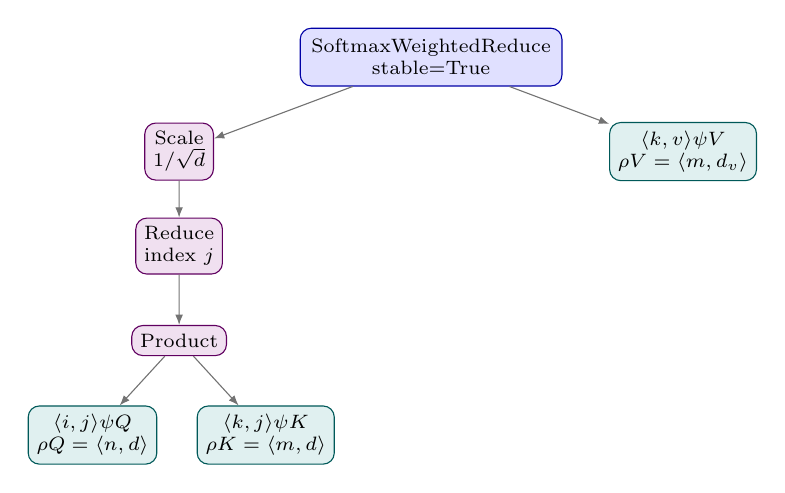
\begin{tikzpicture}[>=Latex,level distance=12mm,
 every node/.style={font=\scriptsize,align=center},
 edge from parent/.style={draw=black!55,-{Latex[length=1.3mm]}},
 level 1/.style={sibling distance=64mm},level 2/.style={sibling distance=33mm},
 level 3/.style={sibling distance=22mm},level 4/.style={sibling distance=22mm},
 root/.style={draw=blue!65!black,fill=blue!12,rounded corners,inner sep=4pt},
 op/.style={draw=violet!75!black,fill=violet!12,rounded corners,inner sep=3pt},
 leaf/.style={draw=teal!70!black,fill=teal!12,rounded corners,inner sep=3pt}]
\node[root] {SoftmaxWeightedReduce\\stable=True}
 child {node[op] {Scale\\$1/\sqrt d$}
   child {node[op] {Reduce\\index $j$}
     child {node[op] {Product}
       child {node[leaf] {$\langle i,j\rangle\psi Q$\\$\rho Q=\langle n,d\rangle$}}
       child {node[leaf] {$\langle k,j\rangle\psi K$\\$\rho K=\langle m,d\rangle$}}
     }
   }
 }
 child {node[leaf] {$\langle k,v\rangle\psi V$\\$\rho V=\langle m,d_v\rangle$}}
 ;
\end{tikzpicture}
\caption{\textbf{Actual restricted semantic AST} reconstructed from the supplied
\texttt{specification()} function and \texttt{typed\_derivation\_trace.json}.
Blue denotes the attention root, purple denotes operations, and teal denotes
$\psi$-indexed leaves. Field labels $k,v$ and the stability flag belong to the
root, rather than additional invented rewrite nodes.}
\label{fig:actual-typed-ast}
\end{figure}

\subsection{Checked stable online summary and numerical contract}
\texttt{stable\_online\_fold()} accepts only the exact supported $\psi$
dependencies and stable scaled reduction. It produces
\texttt{OnlineSummary(score,values,key\_index,value\_index,state)},
with state $\langle a,z,u\rangle$. For one query $i$ and keys processed
through $k$, the online summary has maximum $a$, scaled normalizer $z$,
and value accumulator $u$; its output is $u/z$. The concrete generated
source uses, for each next score $s$ and value component $v$,
\begin{align}
 a'&=\max(a,s), & h&=\begin{cases}0&z=0\\e^{a-a'}&z\ne0\end{cases},
 & f&=e^{s-a'},\\
 z'&=hz+f, & u'_v&=h u_v+f(\langle k,v\rangle\psi V),
 & (\langle i,v\rangle\psi O)&=u_v/z.
\end{align}
The equivalence claim is exact-arithmetic algebra under defined nonempty
extents. Floating-point order, exceptional values, and the backend's
numerical tolerance remain explicit acceptance conditions.

\subsection{Actual $\gamma$-addressed ONF AST}
\texttt{gamma\_lower()} maps the checked summary to
\texttt{LoweredAttention(summary,addresses,ownership)}, with ownership
\texttt{query-disjoint}. Each address is a \texttt{GammaAddress} AST node:
\begin{equation}
\begin{array}{c|c|c}
\text{array}&\psi\text{ selection}&\text{current row-major address}\\ \hline
Q&\langle i,j\rangle\psi Q&(\operatorname{rav}Q)[i d+j]\\
K&\langle k,j\rangle\psi K&(\operatorname{rav}K)[k d+j]\\
V&\langle k,v\rangle\psi V&(\operatorname{rav}V)[k d_v+v]\\
O&\langle i,v\rangle\psi O&(\operatorname{rav}O)[i d_v+v]
\end{array}
\end{equation}
The address mapping is one member of the MoA $\gamma$ family; it is not a
claim that row-major addressing is the only possible layout. The present
\texttt{verify()} checks the expected four address triples and ownership
string. It does not prove correctness for arbitrary layouts.

\begin{figure}[htbp]\centering
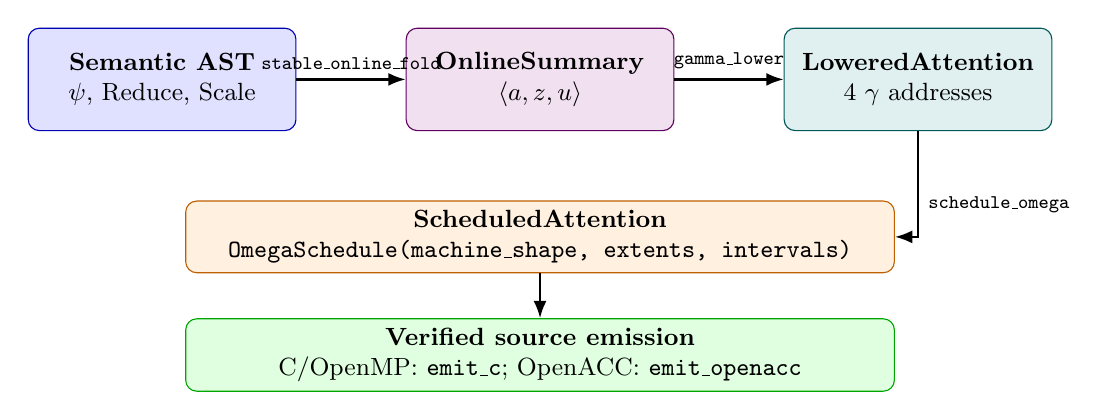
\begin{tikzpicture}[>=Latex,font=\small,
 st/.style={draw,rounded corners,align=center,minimum height=13mm,minimum width=34mm,inner sep=5pt},
 arr/.style={-{Latex[length=2.2mm]},thick}]
\node[st,fill=blue!12,draw=blue!70!black] (a) at (0,0) {\textbf{Semantic AST}\\$\psi$, Reduce, Scale};
\node[st,fill=violet!12,draw=violet!75!black] (b) at (4.8,0) {\textbf{OnlineSummary}\\$\langle a,z,u\rangle$};
\node[st,fill=teal!12,draw=teal!70!black] (c) at (9.6,0) {\textbf{LoweredAttention}\\4 $\gamma$ addresses};
\draw[arr] (a)--node[above,font=\scriptsize]{\texttt{stable\_online\_fold}}(b);
\draw[arr] (b)--node[above,font=\scriptsize]{\texttt{gamma\_lower}}(c);
\node[draw=orange!75!black,fill=orange!12,rounded corners,align=center,minimum width=9cm] (d) at (4.8,-2) {\textbf{ScheduledAttention}\\\texttt{OmegaSchedule(machine\_shape, extents, intervals)}};
\draw[arr] (c.south) |- node[pos=.35,right,font=\scriptsize]{\texttt{schedule\_omega}} (d.east);
\node[draw=green!65!black,fill=green!12,rounded corners,align=center,minimum width=9cm] (e) at (4.8,-3.5) {\textbf{Verified source emission}\\C/OpenMP: \texttt{emit\_c}; OpenACC: \texttt{emit\_openacc}};
\draw[arr] (d)--(e);
\end{tikzpicture}
\caption{The current concrete AST and source-emission chain. The source
supports restricted forward attention and verifies the supported patterns;
this is not a claim of universal automatic normalization, optimal scheduling,
or measured accelerator execution.}
\label{fig:actual-chain}
\end{figure}

\subsection{$\Omega$ ownership, resource constraints, and independent routing audit}
\texttt{OmegaSchedule} stores machine shape, query/key/score/value extents,
and ownership intervals; \texttt{ScheduledAttention} pairs that schedule
with the lowered AST. The basic \texttt{schedule\_omega()} delegates to
\texttt{omega\_lift()} and checks interval coverage. A distinct, additive
resource-constrained planning layer \texttt{ResourceOmegaPlan} permits
heterogeneous query counts and idle machine components; its ownership is
then consumed by the communication certificate and topology constructor.
The abstract machine is a shaped array, not an MPI implementation choice.

For a shaped machine $M$ with $P=\tau(M)$ components, an active owner $p$
with query interval $[b_p,e_p)$ has payload
\begin{equation}
 B_p=(e_p-b_p)d_v w,
 \qquad L_p=(P-1)B_p,
 \qquad L_{\rm total}=\sum_{p:B_p>0}L_p,
\label{eq:nov-linkbytes}
\end{equation}
where $w$ is bytes per value component. The current candidate realization
uses a deterministic owner-rooted nearest-neighbor spanning tree on the
logical machine shape. For each nonempty owner, the route has $P-1$ directed
edges, and its audited link-byte volume agrees with the logical nonlocal
demand. This equality is \emph{not} a measurement of physical DGX link
traffic and does not imply that MPI\_Allgatherv uses this tree.

\begin{figure}[htbp]\centering
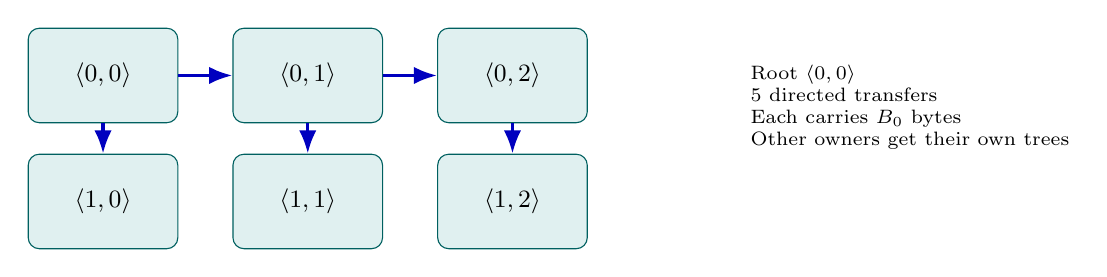
\begin{tikzpicture}[>=Latex,scale=1.0,font=\small]
\foreach \r in {0,1}{\foreach \c in {0,1,2}{
 \pgfmathtruncatemacro{\ord}{3*\r+\c}
 \node[draw=teal!75!black,rounded corners,fill=teal!12,minimum width=19mm,minimum height=12mm] (p\ord) at (2.6*\c,-1.6*\r) {$\langle\r,\c\rangle$};}}
\draw[->,very thick,blue!75!black] (p0)--(p1);
\draw[->,very thick,blue!75!black] (p0)--(p3);
\draw[->,very thick,blue!75!black] (p1)--(p2);
\draw[->,very thick,blue!75!black] (p1)--(p4);
\draw[->,very thick,blue!75!black] (p2)--(p5);
\node[anchor=west,font=\scriptsize,align=left] at (8.1,-.4) {Root $\langle0,0\rangle$\\5 directed transfers\\Each carries $B_0$ bytes\\Other owners get their own trees};
\end{tikzpicture}
\caption{Illustrative logical $\rho M=\langle2,3\rangle$ owner-rooted
nearest-neighbor tree for the first owner. Arrows show a valid directed
spanning tree on the abstract machine; the independent auditor checks
adjacency, receive-before-forward, unique delivery, reachability, hop count,
and traffic accounting.}
\label{fig:nov-tree}
\end{figure}

The independent \texttt{audit\_omega\_topology()} verifies actual owner
coordinates and intervals against the resource plan, correct component and
byte counts, nearest-neighbor transfers, absence of duplicate edges,
receive-before-forward order, complete reachability, maximum hops, and
aggregate traffic. It is intentionally stricter than the topology object's
internal \texttt{verify()} method. The topology layer is currently an
\emph{additive research module}; integration into a general AST lowering
pipeline and physical timing model is still work to be done.

\subsection{Observed regression evidence and outstanding acceptance gates}
On November 3, 2026, the DGX terminal transcript reported
\texttt{Ran 24 tests in 0.033s --- OK} for
\texttt{test\_attention\_omega\_topology.py}. These included valid
heterogeneous and idle ownership, a singleton machine, multidimensional
machine shapes, and deliberate corruptions of routes, dependencies,
intervals, element widths, hop counts, and traffic totals. In particular,
\texttt{test\_self\_consistent\_wrong\_ownership} passed: consistent
aggregate accounting did not mask incorrect ownership. This is a reported
unit-test outcome, \emph{not} a hardware network performance measurement.
An earlier full-suite baseline of 123 tests preceded the topology modules.
Subsequent verified milestones increased the suite to 170 passing tests after
port scheduling, 202 after heterogeneous communication-time prediction,
218 after directed-link contention prediction, and 234 after candidate
schedule selection (see Sections~\ref{sec:nov-verified-communication}
and~\ref{sec:nov-contention-selection}).

\begin{center}\small
\begin{tabular}{p{.42\linewidth}p{.48\linewidth}}\toprule
\textbf{Current evidence} & \textbf{Still required for SC27 acceptance}\\\midrule
Typed forward-attention AST, restricted checked summary rule, four $\gamma$
addresses & General $\psi$-reduction/normalization and broader semantic
AST coverage\\
C/OpenMP and OpenACC source emitters in inspected Python source & Independent
compilation, execution, and numerical validation of all emitted backends
on target systems\\
Basic and resource-constrained $\Omega$ ownership, communication certificates
and topology auditor & Integrate all certificates into the compiler pass
trace and establish composition of correctness obligations\\
234 passing compiler tests on DGX (latest checkpoint), including independent
contention and schedule-selection tests & Prospective calibrated time/energy
predictions, physical hardware measurements, and exhaustive small-case optimality certificates\\
Four hand-derived attention/Transformer studies as targets & Compiler
reproduction of forward, backward, decode, and Transformer-block
implementations and their predictions\\\bottomrule
\end{tabular}
\end{center}

\paragraph{Reproducibility and source boundary.}
The source text of \texttt{moa\_typed\_ir.py} and the JSON derivation trace
were supplied verbatim in the research conversation; the newer topology
modules and test results were supplied during the preceding DGX collaboration.
The current working repository is
\url{https://github.com/womenflyplanes/moa-compiler}. The manuscript does not
assert that all current DGX files were independently retrieved or that a
post-November-3 commit was pushed. The November 3 local commit identifiers for the topology/scheduling,
heterogeneous timing, contention prediction, and candidate selection
milestones are \texttt{f994221}, \texttt{c62d214}, \texttt{faf06be},
and \texttt{018bc83}, respectively; none is claimed here to have been
pushed to a remote.
Archive the full test transcript and exact repository state before submission.


\clearpage
\section{Verified November compiler extension: $\Omega$ port scheduling and heterogeneous communication time}
\label{sec:nov-verified-communication}
This section reports the subsequent November 3, 2026 DGX-head-node
compiler development checkpoint. It extends the typed forward-attention
resource-constrained $\Omega$ ownership and topology described in
Section~\ref{sec:november-integration}; it does not alter the earlier
hand-derived attention implementations or establish end-to-end MPI execution.
The two local commits are \texttt{f994221} (audited topology and port
scheduling) and \texttt{c62d214} (heterogeneous time model, independent
auditor, and tests), on branch \texttt{develop/mac-compiler-integration}.

\subsection{From $\Omega$ ownership to legal port-constrained stages}
Let $M=\rho(\mathrm{machine})$ and let the resource plan assign each active
owner $p\in\iota(M)$ an output interval $[b_p,e_p)$, with payload
$B_p=(e_p-b_p)d_v w$ bytes. The topology constructor produces an
owner-rooted nearest-neighbor spanning tree on the abstract shaped
machine for each nonempty owner. The route is a \emph{candidate logical
realization}, not a physical network topology or a statement about the
implementation of \texttt{MPI\_Allgatherv}. For each owner, its route has
$\tau(M)-1$ edges; hence the logical aggregate link volume is
\begin{equation}
 L_{\mathrm{logical}}=\sum_{p:B_p>0}(\tau(M)-1)B_p.
 \label{eq:nov39-linkbytes}
\end{equation}
A deterministic greedy scheduler partitions the transfers into ordered
stages $S_0,\ldots,S_{k-1}$. In any stage, each parent initiates at most
$q$ outgoing transfers; a receiver may forward a payload only in a
\emph{subsequent} stage. The independent schedule auditor reconstructs
expected transfers from the ownership plan and topology, then checks
exact transfer coverage, per-parent port limits, receive-before-forward,
reachability, machine shape, stage accounting, and logical link bytes.
The resulting schedule is legal for the specified abstract constraints;
minimal stage count has not been proved.

\subsection{A conditional time functional over the verified stages}
For each scheduled transfer $e$ carrying $B_e$ bytes on directed link
$\ell(e)$, assign finite nonnegative latency $\alpha_{\ell(e)}$ and
finite strictly positive effective bandwidth $\beta_{\ell(e)}$.
The transfer-time model is
\begin{equation}
 t_e=\alpha_{\ell(e)}+\frac{B_e}{\beta_{\ell(e)}}.
 \label{eq:nov39-transfer}
\end{equation}
Under the explicit assumptions that transfers in one stage execute
concurrently without additional contention, and stages execute in
sequence, the conditional prediction is
\begin{equation}
 \boxed{T_{\mathrm{comm}}=\sum_{s=0}^{k-1}
 \max_{e\in S_s}\left(\alpha_{\ell(e)}+
 \frac{B_e}{\beta_{\ell(e)}}\right).}
 \label{eq:nov39-time}
\end{equation}
An empty stage contributes zero, and a singleton machine with no
communication has $T_{\mathrm{comm}}=0$. The uniform-link fallback
assigns the same $(\alpha,\beta)$ to every required directed link.
Unlike the earlier fixed-payload broadcast expression in
Equation~\eqref{eq:v14hetero}, Equation~\eqref{eq:nov39-time}
allows owner-dependent payload sizes. It is not a calibrated physical
network model: incoming-port limits, simultaneous use of shared links,
protocol costs, congestion, and computation--communication overlap are
not yet represented.

\begin{figure}[htbp]\centering
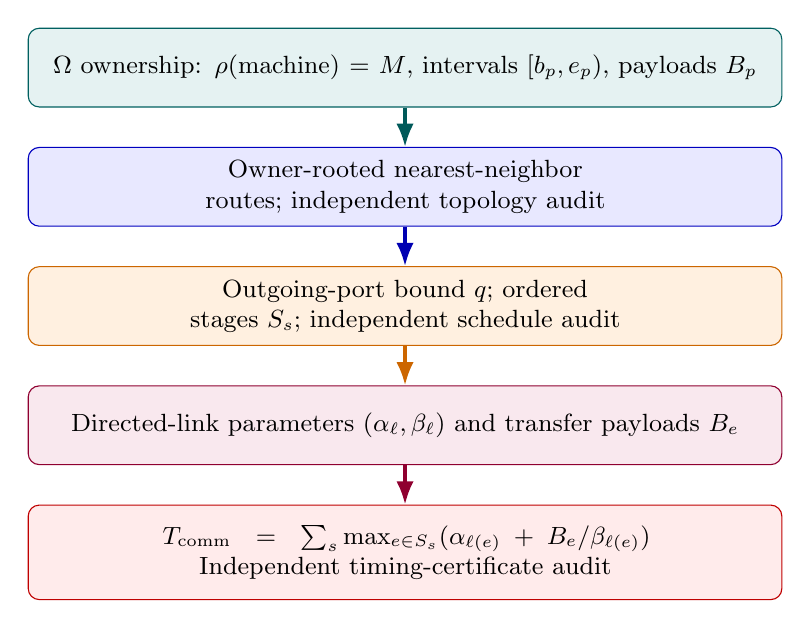
\begin{tikzpicture}[>=Latex,node distance=5mm,font=\small,
 every node/.style={align=center}]
\node[draw=teal!75!black,fill=teal!10,rounded corners,
 text width=.77\linewidth,minimum height=10mm] (owner)
 {$\Omega$ ownership: $\rho(\mathrm{machine})=M$, intervals $[b_p,e_p)$, payloads $B_p$};
\node[draw=blue!75!black,fill=blue!9,rounded corners,
 text width=.77\linewidth,minimum height=10mm,below=of owner] (route)
 {Owner-rooted nearest-neighbor routes; independent topology audit};
\node[draw=orange!80!black,fill=orange!12,rounded corners,
 text width=.77\linewidth,minimum height=10mm,below=of route] (schedule)
 {Outgoing-port bound $q$; ordered stages $S_s$; independent schedule audit};
\node[draw=purple!75!black,fill=purple!9,rounded corners,
 text width=.77\linewidth,minimum height=10mm,below=of schedule] (links)
 {Directed-link parameters $(\alpha_\ell,\beta_\ell)$ and transfer payloads $B_e$};
\node[draw=red!75!black,fill=red!8,rounded corners,
 text width=.77\linewidth,minimum height=12mm,below=of links] (time)
 {$T_{\mathrm{comm}}=\sum_s\max_{e\in S_s}(\alpha_{\ell(e)}+B_e/\beta_{\ell(e)})$\\Independent timing-certificate audit};
\draw[->,very thick,teal!70!black] (owner)--(route);
\draw[->,very thick,blue!70!black] (route)--(schedule);
\draw[->,very thick,orange!80!black] (schedule)--(links);
\draw[->,very thick,purple!75!black] (links)--(time);
\end{tikzpicture}
\caption{Verified MoA machine-shape communication derivation in the
November compiler prototype. Each stage has independently checkable
ownership, transfer, or timing obligations. The final time is conditional
on the stated stage-concurrency assumptions, not measured hardware time.}
\label{fig:nov39-comm-pipeline}
\end{figure}

\subsection{DGX-head-node regression evidence}
The complete \texttt{tests/universal\_ir} suite reported
\texttt{Ran 202 tests in 1.885s --- OK} on \texttt{dgx-head01}.
The dedicated timing module reported 32 passing tests in 0.073 seconds,
including 7 ordinary cases, 11 invalid-parameter cases, and 14
adversarial certificate mutations. An independently constructed auditor
checks the original ownership and schedule, exact link-key coverage,
finite parameter domains, each stage maximum, and total time. It rejects
self-consistent but incorrect stage and total times. These are reported
software tests on the head node, not network timing experiments.

\begin{table}[htbp]\centering\small
\caption{Verified logical schedules for heterogeneous $\Omega$ ownership.
The stages are deterministic greedy outputs, not proven optima.}
\label{tab:nov39-schedules}
\begin{tabular}{lrrrr}\toprule
Machine shape and ownership & $q=1$ & $q=2$ & $q=100$ & Link bytes\\\midrule
$\langle2,3\rangle$, counts $(1,2,1,1,1,1)$ & 11 & 6 & 3 & 840\\
$\langle2,3\rangle$, counts $(3,0,0,0,0,0)$ & 3 & 3 & 3 & 480\\
$\langle2,2,2\rangle$, all counts 1 & 12 & 6 & 3 & 896\\
$\langle1\rangle$, count 4 & 0 & 0 & 0 & 0\\\bottomrule
\end{tabular}
\end{table}

For $M=\langle2,3\rangle$, counts $(1,2,1,1,1,1)$,
$q=1$, and $L_{\mathrm{logical}}=840$ bytes, the uniform-link inputs
$\alpha=2\,\mu\mathrm{s}$ and $\beta=10\,\mathrm{GB/s}$ yield
$T_{\mathrm{comm}}=22.036\,\mu\mathrm{s}$ across 11 stages.
Replacing the parameters on directed link
$\langle0,0\rangle\rightarrow\langle0,1\rangle$ with
$\alpha=8\,\mu\mathrm{s}$ and $\beta=1\,\mathrm{GB/s}$ yields
$34.0744\,\mu\mathrm{s}$ with the \emph{same} ownership, stages, and
840 logical link bytes. The predicted increase is approximately 54.6\%.
Both certificates passed the independent audit. These are analytic
outputs of an assumed link model, not DGX latency observations.

\paragraph{Acceptance boundary and next step.}
At this Step 102 checkpoint, the evidence supported a reproducible, finite,
audited compiler extension from $\Omega$ ownership through topology, legal
port scheduling, and conditional heterogeneous communication time. Subsequent
Steps 103--104 add logical directed-link contention and audited candidate
selection (Section~\ref{sec:nov-contention-selection}). Physical-network
accuracy, time-optimal scheduling, and compiler reproduction of all four
hand-derived attention and Transformer implementations remain open.


\clearpage
\section{Directed-link contention and predictive $\Omega$ schedule selection (Steps 103--104)}
\label{sec:nov-contention-selection}
\paragraph{Scope and invariants.}
The November 3, 2026 extension retains the previously derived MoA
$\psi$-indexed computation, $\Omega$ query ownership, owner-rooted logical
communication topology, and exact transfer multiset. A transfer is identified
by its owner coordinate, parent and child machine coordinates, and payload
size. Legal schedules are stage partitions of these transfers respecting
receive-before-forward, parent outgoing-port limits, unique delivery, and
complete reachability. Stage rearrangement changes neither denotational
semantics nor the logical total link bytes. Independent auditors check the
schedule against the original topology rather than trusting its constructor.

\paragraph{Conditional contention model (Step 103).}
For a directed logical link $\ell$ used in stage $s$, define
$B_{s,\ell}=\sum_{e\in E_{s,\ell}}b_e$, where $E_{s,\ell}$ is the multiset
of transfers assigned to that link and stage and $b_e$ is the transfer's
payload in bytes. With assumed nonnegative latency $\alpha_\ell$ and
positive bandwidth $\beta_\ell$, the model predicts
\begin{equation}
  T_s=\max_{\ell:\,E_{s,\ell}\ne\varnothing}
       \left(\alpha_\ell+\frac{B_{s,\ell}}{\beta_\ell}\right),
  \qquad T_{\mathrm{comm}}=\sum_s T_s.
  \label{eq:step103-contention}
\end{equation}
Empty stages contribute zero. The sum aggregates simultaneous logical
transfers using the same directed link; the maximum assumes concurrency
across distinct links within a stage. This is a \emph{conditional logical-link
model}, not a calibrated physical DGX network model. It omits unmodeled
shared physical paths, protocol overhead, computation overlap, and network
congestion beyond the defined directed-link aggregation. The Step 103
implementation and independent contention auditor are preserved in local
commit \texttt{faf06be}.

\paragraph{Deterministic candidate selection (Step 104).}
Let $\mathcal{S}_{\mathrm{legal}}$ be the set of schedules admitted by the
independent port-schedule auditor. The implementation evaluates a finite
candidate subset $\mathcal{C}\subseteq\mathcal{S}_{\mathrm{legal}}$
containing the original deterministic baseline $S_0$ and twelve alternatives:
six priority rules (large payload first, small payload first, slowest
individual transfer first, fastest first, link order, and owner order),
each with and without a same-directed-link-per-stage exclusion rule.
Every candidate is independently audited for schedule legality and
contention-time accounting. The selection is
\begin{equation}
 S^*\in\underset{S\in\mathcal{C}}{\operatorname{arg\,min}}\;
 T_{\mathrm{comm}}(S),\qquad
 T_{\mathrm{comm}}(S^*)\le T_{\mathrm{comm}}(S_0).
 \label{eq:step104-selection}
\end{equation}
Ties retain the earlier selected candidate; the baseline is initially
selected. The inequality is guaranteed for successfully audited candidates
under the specified prediction model, \emph{not} for physical runtime.
The candidate subset is heuristic and finite; the procedure does not
establish optimality over all legal schedules. The Step 104 implementation
and regression tests are preserved in local commit \texttt{018bc83}.

\begin{figure}[htbp]
\centering
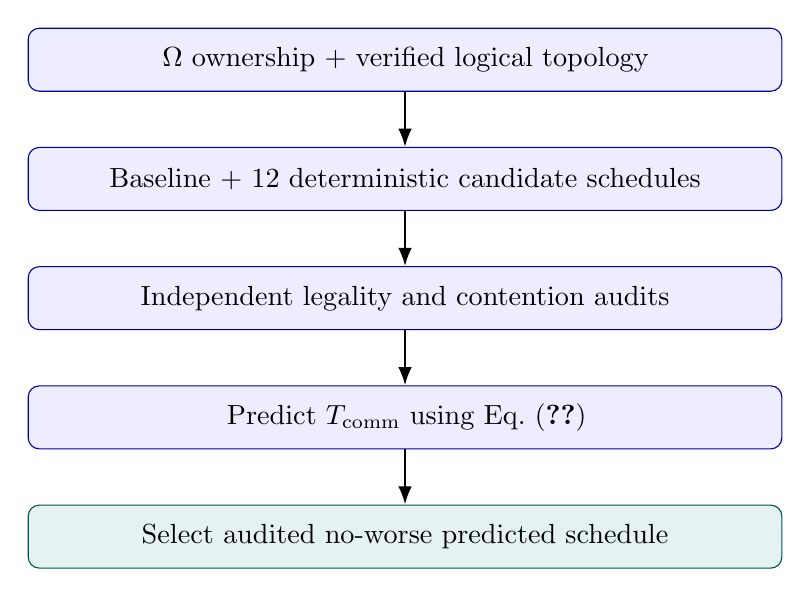
\begin{tikzpicture}[>=Latex, node distance=7mm,
  b/.style={draw=blue!65!black,rounded corners,fill=blue!7,
  align=center,text width=0.77\linewidth,minimum height=8mm},
  g/.style={draw=teal!65!black,rounded corners,fill=teal!10,
  align=center,text width=0.77\linewidth,minimum height=8mm}]
\node[b] (o) {$\Omega$ ownership + verified logical topology};
\node[b,below=of o] (c) {Baseline + 12 deterministic candidate schedules};
\node[b,below=of c] (a) {Independent legality and contention audits};
\node[b,below=of a] (p) {Predict $T_{\mathrm{comm}}$ using Eq.~\eqref{eq:step103-contention}};
\node[g,below=of p] (s) {Select audited no-worse predicted schedule};
\draw[->,thick] (o)--(c); \draw[->,thick] (c)--(a);
\draw[->,thick] (a)--(p); \draw[->,thick] (p)--(s);
\end{tikzpicture}
\caption{Step 104: MoA-derived machine ownership and logical dependencies
constrain the candidate schedules. Independent audits precede model-based
selection. This is not hardware-autotuning or an exhaustive optimality proof.}
\label{fig:step104-selection}
\end{figure}

\paragraph{Reproducible heterogeneous-link example.}
For attention descriptor \texttt{Work(7,5,4,3)}, machine shape
$\langle2,3\rangle$, query ownership counts
$\langle1,2,1,1,1,1\rangle$, and two outgoing ports per parent,
all logical links use $\alpha=2\,\mu\mathrm{s}$ and
$\beta=10\,\mathrm{GB/s}$ except the directed link
$\langle1,1\rangle\rightarrow\langle1,2\rangle$, whose bandwidth is
$1\,\mathrm{GB/s}$. The scheduler examines thirteen candidates, selects
\texttt{slow\_first:shared\_links\_allowed}, and retains six stages,
$\langle12,8,4,3,2,1\rangle$ transfers per stage, and 840 logical
link bytes. The independent schedule and contention auditors both pass.

\begin{table}[htbp]\centering\small
\caption{Step 104 stage times under the conditional directed-link model.
A negative saving denotes a slower selected stage.}
\label{tab:step104-stages}
\begin{tabular}{rrrr}\toprule
Stage & Baseline ($\mu$s) & Selected ($\mu$s) & Saved ($\mu$s)\\\midrule
0 & 2.0048 & 2.0240 & $-0.0192$\\
1 & 2.0480 & 2.0240 & $+0.0240$\\
2 & 2.0048 & 2.0024 & $+0.0024$\\
3 & 2.0024 & 2.0024 & $0$\\
4 & 2.0024 & 2.0024 & $0$\\
5 & 2.0024 & 2.0024 & $0$\\\midrule
Total & 12.0648 & 12.0576 & $+0.0072$\\\bottomrule
\end{tabular}
\end{table}

The schedule advances owner $\langle1,1\rangle$'s 24-byte transfer
$\langle1,1\rangle\rightarrow\langle1,2\rangle$ from stage 1 to stage 0
and postpones its 24-byte transfer to $\langle1,0\rangle$ from stage 0
to stage 1. It also advances owner $\langle0,1\rangle$'s 48-byte transfer
$\langle0,1\rangle\rightarrow\langle1,1\rangle$ from stage 2 to stage 1,
while postponing owner $\langle0,0\rangle$'s 24-byte transfer on the same
directed link from stage 1 to stage 2. Consequently, stage 0 becomes
$0.0192\,\mu$s slower, while stages 1 and 2 save $0.0240$ and
$0.0024\,\mu$s. The net predicted saving is $0.0072\,\mu$s
(approximately $0.0597\%$ of baseline). This illustrates why minimizing
each stage independently need not minimize the sum under interstage
transfer dependencies.

\paragraph{Regression evidence and limits.}
The Step 103 contention model added 16 tests and the full
\texttt{tests/universal\_ir} suite passed 218 tests. Step 104 added
16 further tests covering the numerical improvement, stage reassignment,
determinism, alternative machine shapes, port counts, uniform and
heterogeneous links, zero and large latency, and corrupted-result
rejection. The November 3 DGX-head-node transcript reports
\texttt{Ran 234 tests in 2.308s --- OK}. These are software regression
results, not measurements of communication time on DGX devices.
The four hand-derived attention/Transformer reference implementations
remain acceptance targets for automated compiler reproduction. Future
work includes bounded exhaustive search with independently checkable
optimality certificates for small machine shapes, scaling studies,
calibrated physical-network prediction, and actual OpenMP/OpenACC/MPI
execution validation.

\clearpage

% Step 108: SC27 compiler architecture section
% Standalone inclusion: \input{moa_sc27_compiler_architecture_step108}
% Required in the main document preamble:
% \usepackage{amsmath,amssymb}
% \usepackage{tikz}
% \usetikzlibrary{arrows.meta,positioning,shapes.geometric,fit,calc,matrix}
% \usepackage{xcolor}
% Figures use TikZ only: no external image files.
% This is an includable section, not a standalone document.
\section{From MoA Semantics to Verified Machine-Array Communication}
\label{step108:sec:moa-compiler-architecture}

The Mathematics of Arrays (MoA) provides a single mathematical language for
specifying shaped-array computations, deriving their indexed behavior, lowering
that behavior to addresses, and assigning work and communication to a shaped
machine.  Our implementation demonstrates portions of this progression through
independently checkable compiler components.  The current implementation is a
\emph{restricted compiler prototype}, not yet a general-purpose MoA compiler.
In particular, the earlier attention implementations and their hardware results
were derived and programmed by hand; they must not be presented as outputs of
this compiler.


\subsection{The MoA compilation contract: portable, scalable, verifiable}
\label{step108:subsec:moa-compiler-contract}

The central claim of this research is methodological: \emph{one MoA
mathematical derivation can be specialized to different shaped machines
without changing the meaning of the computation}.  Portability follows
from separating $\psi$ semantics from $\gamma$ addressing and $\Omega$
ownership; scalability is addressed by expressing the machine itself as
an array whose shape and resources may change; verifiability comes from
checking invariants at each transformation boundary.  None of these
properties, by itself, establishes performance portability on all
hardware.  Instead, performance is a prospective, explicitly
parameterized prediction to be validated by measurement.

For an array $A$, its shape and component count satisfy
\begin{equation}
 \rho A=\langle s_0,\ldots,s_{r-1}\rangle,\qquad
 \delta(A)=\tau(\rho A)=r,\qquad
 \tau(A)=\prod_{k=0}^{r-1}s_k .
 \label{step108:eq:moa-core-invariants}
\end{equation}
Here $\delta(A)$ is a scalar dimensionality, and $\tau(A)$ is the
number of components.  A rank-one array remains a vector; a rank-two
array is a matrix.  Index selection obeys the MoA reconstruction
identity
\begin{equation}
       (\iota(\rho A)\ \psi\ A)\equiv A .
       \label{step108:eq:moa-reconstruction}
\end{equation}
The mathematical obligation of $\Omega$ lifting is to preserve the
logical array and its components while changing the ownership and
realization of those components:
\begin{equation}
 \tau(A_{\mathrm{logical}})=\tau(A_{\mathrm{lifted,logical}}),
 \qquad
 \rho M=\langle p_0,\ldots,p_{r-1}\rangle .
 \label{step108:eq:moa-lifting-invariant}
\end{equation}
Physical padding or replicated storage is accounted for separately;
it must not be silently equated with logical $\tau(A)$.

\begin{figure}[t]
\centering
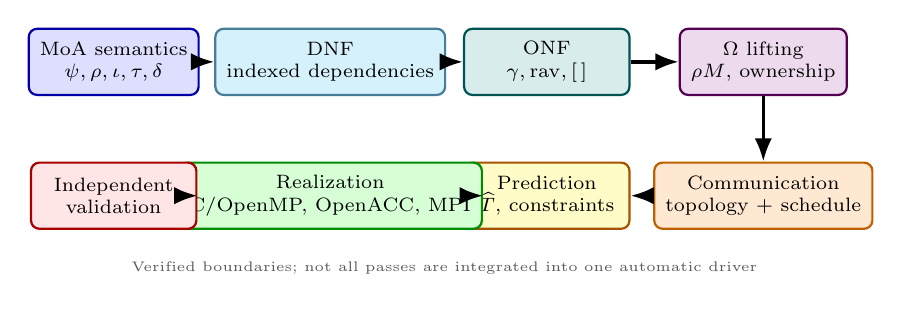
\begin{tikzpicture}[>=Latex, font=\scriptsize,
  every node/.style={align=center},
  block/.style={draw,rounded corners=3pt,minimum width=2.1cm,
    minimum height=0.84cm,inner sep=4pt,thick},
  arr/.style={->,very thick}]
\node[block,fill=blue!13,draw=blue!65!black] (sem) at (0,0)
  {MoA semantics\\$\psi,\rho,\iota,\tau,\delta$};
\node[block,fill=cyan!17,draw=cyan!55!black] (dnf) at (2.75,0)
  {DNF\\indexed dependencies};
\node[block,fill=teal!15,draw=teal!65!black] (onf) at (5.5,0)
  {ONF\\$\gamma,\operatorname{rav},[\,]$};
\node[block,fill=violet!14,draw=violet!65!black] (omega) at (8.25,0)
  {$\Omega$ lifting\\$\rho M$, ownership};
\node[block,fill=orange!18,draw=orange!75!black] (comm) at (8.25,-1.7)
  {Communication\\topology + schedule};
\node[block,fill=yellow!22,draw=orange!65!black] (pred) at (5.5,-1.7)
  {Prediction\\$\widehat T$, constraints};
\node[block,fill=green!16,draw=green!55!black] (emit) at (2.75,-1.7)
  {Realization\\C/OpenMP, OpenACC, MPI};
\node[block,fill=red!10,draw=red!65!black] (valid) at (0,-1.7)
  {Independent\\validation};
\draw[arr] (sem)--(dnf);
\draw[arr] (dnf)--(onf);
\draw[arr] (onf)--(omega);
\draw[arr] (omega)--(comm);
\draw[arr] (comm)--(pred);
\draw[arr] (pred)--(emit);
\draw[arr] (emit)--(valid);
\node[font=\tiny,text=black!65] at (4.2,-2.62)
 {Verified boundaries; not all passes are integrated into one automatic driver};
\end{tikzpicture}
\caption{The MoA research program: semantics to DNF, ONF,
$\Omega$ machine ownership, communication, prospective prediction,
realization, and validation. Colors distinguish mathematical,
machine-mapping, predictive, and validation responsibilities. The
diagram expresses the architecture and the currently implemented
bounded components, not a claim that every pass is integrated.}
\label{step108:fig:moa-compiler-pipeline}
\end{figure}

\subsection{Typed $\psi$ specification and restricted lowering}
\label{step108:subsec:typed-psi}

The typed forward-attention intermediate representation represents arrays by
shape, selections by $\psi$, and the score expression by a product, reduction,
and scale.  With
$\rho Q=\langle n,d\rangle$,
$\rho K=\langle m,d\rangle$, and
$\rho V=\langle m,d_v\rangle$, its score dependence is
\begin{equation}
  s_{ik}=\frac{1}{\sqrt d}
  \mathop{+\mathrm{red}}_{j=0}^{d-1}
  \left((\langle i,j\rangle\,\psi\,Q)
        \times(\langle k,j\rangle\,\psi\,K)\right).
  \label{step108:eq:moa-attention-score}
\end{equation}
The corresponding stable softmax-weighted reduction selects
$\langle k,v\rangle\,\psi\,V$ over the key index $k$ to produce
$\langle i,v\rangle\,\psi\,O$.
The implementation recognizes this \emph{specific} typed dependence pattern
and converts it to an online summary with state $\langle a,z,u\rangle$.
It rejects unsupported expressions rather than claiming a general $\psi$
rewrite system.  The summary is subsequently lowered to explicit $\gamma$
addresses for $Q$, $K$, $V$, and $O$.  For the sequential layout used by this
backend,
\begin{equation}
  \gamma(\langle i,v\rangle,\rho O)=i d_v+v,
  \qquad \rho O=\langle n,d_v\rangle.
  \label{step108:eq:moa-output-gamma}
\end{equation}
The typed implementation emits C with optional OpenMP and an OpenACC source
backend.  Source generation alone is not evidence of successful execution on a
particular accelerator, nor does its structural verifier prove universal
floating-point equivalence.


\paragraph{A typed AST, not a copied kernel.}
The implemented restricted attention IR contains explicit constructors
\texttt{Array}, \texttt{Psi}, \texttt{Product}, \texttt{Reduce},
\texttt{Scale}, and \texttt{SoftmaxWeightedReduce}.  The stable online
rewrite checks the precise indexed pattern before constructing
\texttt{OnlineSummary}; \texttt{gamma\_lower} produces
\texttt{GammaAddress} nodes.  Figure~\ref{step108:fig:moa-typed-ast}
makes these transformations visible.

\begin{figure}[t]
\centering
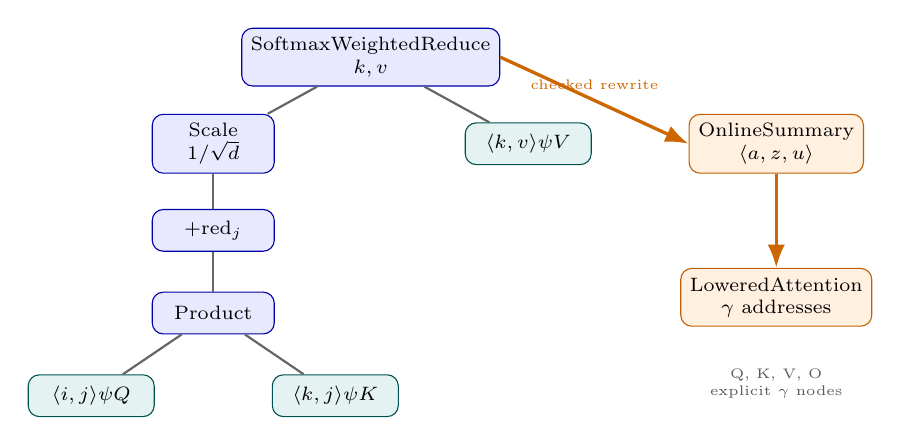
\begin{tikzpicture}[>=Latex,font=\scriptsize,
  ast/.style={draw=blue!65!black,fill=blue!9,rounded corners,
    minimum width=1.55cm,minimum height=.53cm,align=center},
  leaf/.style={draw=teal!65!black,fill=teal!10,rounded corners,
    minimum width=1.6cm,minimum height=.53cm,align=center},
  trans/.style={draw=orange!75!black,fill=orange!12,rounded corners,
    minimum width=2.15cm,minimum height=.7cm,align=center},
  edge/.style={draw=black!60,thick}]
\node[ast] (root) at (0,0) {SoftmaxWeightedReduce\\$k,v$};
\node[ast] (scale) at (-2,-1.1) {Scale\\$1/\sqrt d$};
\node[leaf] (values) at (2,-1.1) {$\langle k,v\rangle\psi V$};
\node[ast] (reduce) at (-2,-2.2) {$+\mathrm{red}_j$};
\node[ast] (product) at (-2,-3.25) {Product};
\node[leaf] (q) at (-3.55,-4.3) {$\langle i,j\rangle\psi Q$};
\node[leaf] (k) at (-.45,-4.3) {$\langle k,j\rangle\psi K$};
\foreach \a/\b in {root/scale,root/values,scale/reduce,reduce/product,product/q,product/k}
 \draw[edge] (\a)--(\b);
\node[trans] (online) at (5.15,-1.1) {OnlineSummary\\$\langle a,z,u\rangle$};
\node[trans] (gamma) at (5.15,-3.05) {LoweredAttention\\$\gamma$ addresses};
\draw[->,very thick,orange!80!black] (root.east)
  -- node[above,font=\tiny] {checked rewrite} (online.west);
\draw[->,very thick,orange!80!black] (online)--(gamma);
\node[font=\tiny,text=black!65,align=center] at (5.15,-4.15)
  {Q, K, V, O\\explicit $\gamma$ nodes};
\end{tikzpicture}
\caption{Typed MoA attention abstract syntax tree (AST) and the
restricted verified-pattern transformation. The AST preserves
$\psi$ dependencies; the right-hand nodes represent the online
summary and addressed lowering. Structural checks do not by
themselves prove universal floating-point equivalence.}
\label{step108:fig:moa-typed-ast}
\end{figure}

For each fixed query index $i$, the stable online summary begins with
$a_0=-\infty$, $z_0=0$, and $\langle v\rangle\psi u_0=0$.
For each key index $k$, let
\begin{align}
 a_{k+1}&=\max(a_k,s_{ik}),\\
 w_k&=
 \begin{cases}
 0,&z_k=0,\\
 \exp(a_k-a_{k+1}),&z_k\ne0,
 \end{cases}
 &f_k&=\exp(s_{ik}-a_{k+1}),\\
 z_{k+1}&=w_kz_k+f_k,\\
 \langle v\rangle\psi u_{k+1}
   &=w_k(\langle v\rangle\psi u_k)
     +f_k(\langle k,v\rangle\psi V),\\
 \langle i,v\rangle\psi O
   &=(\langle v\rangle\psi u_m)/z_m .
 \label{step108:eq:moa-online-output}
\end{align}
These recurrences explain the code-emission rule and avoid
materializing the full score array.  They describe real-arithmetic
semantics; floating-point order and rounding require their own
validation.

\subsection{$\Omega$ ownership on a shaped machine}
\label{step108:subsec:omega-ownership}

Let the target machine be a shaped array $M$ with
$\rho M=\langle p_0,\ldots,p_{r-1}\rangle$ and
$P=\tau(M)=\prod(\rho M)$.  The compiler enumerates machine coordinates
using $\iota(\rho M)$ in a specified sequential $\gamma$ order.  For ordinal
$q\in\{0,\ldots,P-1\}$, it assigns the half-open query interval
\begin{equation}
  I_q=\left[
    \left\lfloor\frac{nq}{P}\right\rfloor,
    \left\lfloor\frac{n(q+1)}{P}\right\rfloor
  \right).
  \label{step108:eq:moa-omega-interval}
\end{equation}
Empty intervals are permitted when $P>n$.  The verifier checks that these
intervals cover every query index exactly once, in order, and preserve the
number of output components:
\begin{equation}
  \sum_{q=0}^{P-1}|I_q|d_v=nd_v=\tau(O).
  \label{step108:eq:moa-output-conservation}
\end{equation}
A multidimensional bridge maps each query interval to the output rectangle
$I_q\times[0,d_v)$ at its machine coordinate.  It checks output ownership,
logical coverage, the machine shape, and sequential $\gamma$ addresses.  Its
resource checks concern output storage; replicated inputs, temporary arrays,
communication buffers, and physical execution time are outside this bridge's
scope.  This ownership rule balances query counts but is not a heterogeneous
placement optimizer.


\begin{figure}[t]
\centering
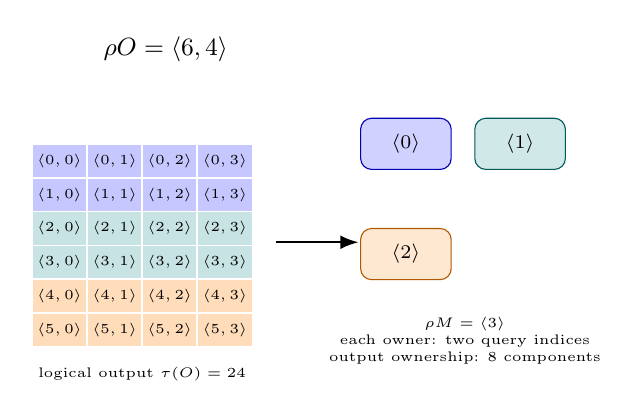
\begin{tikzpicture}[font=\scriptsize,>=Latex]
\node[font=\small\bfseries] at (1.7,1.2)
 {$\rho O=\langle 6,4\rangle$};
\foreach \i in {0,...,5}{
 \foreach \j in {0,...,3}{
  \pgfmathtruncatemacro{\owner}{int(\i/2)}
  \ifnum\owner=0 \def\shade{blue!22}\fi
  \ifnum\owner=1 \def\shade{teal!22}\fi
  \ifnum\owner=2 \def\shade{orange!27}\fi
  \fill[\shade] (\j*.7,-\i*.43) rectangle ++(.7,-.43);
  \draw[white,line width=.6pt] (\j*.7,-\i*.43) rectangle ++(.7,-.43);
  \node[font=\tiny] at (\j*.7+.35,-\i*.43-.215) {$\langle\i,\j\rangle$};
 }
}
\node[font=\tiny] at (1.4,-2.92) {logical output $\tau(O)=24$};
\draw[->,thick] (3.1,-1.25)--(4.15,-1.25);
\foreach \r/\x/\y/\color in {0/4.75/0/blue,1/6.2/0/teal,2/4.75/-1.4/orange}{
 \node[draw=\color!70!black,fill=\color!18,
       rounded corners,minimum width=1.15cm,
       minimum height=.65cm] (m\r) at (\x,\y)
       {$\langle\r\rangle$};
}
\node[font=\tiny,align=center] at (5.5,-2.5)
 {$\rho M=\langle 3\rangle$\\
  each owner: two query indices\\
  output ownership: $8$ components};
\end{tikzpicture}
\caption{Illustrative $\Omega$ lifting of an output of shape
$\langle6,4\rangle$ onto a machine of shape $\langle3\rangle$.
The colors encode disjoint ownership of logical output components,
not separate mathematical arrays or physical memory addresses.
The implemented bridge checks the corresponding rectangular
ownership and $\gamma$ addressing.}
\label{step108:fig:moa-omega-ownership}
\end{figure}

\subsection{Logical resource and communication certificates}
\label{step108:subsec:communication-certificate}

The resource certificate counts, for each machine component, owned output
components, score dot products, score multiplications and additions, value
accumulations, and online-summary components.  These are exact \emph{logical}
counts for the specified attention shape and ownership, not measured time,
power, energy, or memory traffic.

A separate communication module assumes complete read-only copies of $Q$,
$K$, and $V$ on each component and an \texttt{MPI\_Allgatherv} contract that
makes the complete output $O$ available everywhere.  If component $q$ owns
$c_q=|I_q|d_v$ output components, then
\begin{equation}
  \sum_q c_q=N,\qquad N=\tau(O).
\end{equation}
Each component's complete output has $N$ components, while its nonlocal
requirement is $N-c_q$.  Therefore the aggregate logical nonlocal requirement
is exactly
\begin{equation}
  \sum_{q=0}^{P-1}(N-c_q)=(P-1)N,
  \qquad B_{\mathrm{logical}}=(P-1)N b,
  \label{step108:eq:moa-logical-communication}
\end{equation}
where $b$ is the number of bytes per output component.  The implementation
derives collective counts and displacements from the ownership intervals and
cross-checks them against an independent MPI emitter.  Equation
\eqref{step108:eq:moa-logical-communication} describes a logical data requirement,
\emph{not} the physical bytes, message count, routing, or collective algorithm
used by a particular MPI library.  It excludes the initial replication cost
of $Q$, $K$, and $V$.

\subsection{Derived abstract topology and legal stage scheduling}
\label{step108:subsec:omega-scheduling}

For each nonempty owner interval, the topology module constructs a
deterministic breadth-first spanning tree over nearest neighbors of the shaped
machine array.  Its edges are directed from an already reached component to
a newly reached component.  A tree for owner $q$ has $P-1$ transfers of its
payload of $c_qb$ bytes, giving the abstract link-volume identity
\begin{equation}
  B_{\mathrm{tree}}=\sum_{q:c_q>0}(P-1)c_qb=(P-1)Nb.
  \label{step108:eq:moa-tree-volume}
\end{equation}
This is a \emph{candidate} allgather realization on an abstract nearest-neighbor
machine array, not a reconstruction of the physical DGX network or MPI's
chosen collective algorithm.

The port scheduler turns these directed transfers into discrete stages.  For
stage $s$, let $E_s$ denote its transfers, and let $p_{\mathrm{out}}$ be the
outgoing-port limit.  Legality requires
\begin{equation}
  \forall x\in\iota(\rho M):\quad
  \left|\{e\in E_s:\operatorname{parent}(e)=x\}\right|
  \le p_{\mathrm{out}}.
  \label{step108:eq:moa-port-constraint}
\end{equation}
A component receiving an owner's payload in stage $s$ cannot forward that
payload until a subsequent stage.  The scheduler is deterministic and greedy;
it preserves the required transfer volume and checks eventual delivery, but
does not certify minimum stage count.  A separate audit checks full topology,
dependency, and reachability conditions.  The basic scheduler does not model
incoming-port restrictions or contention.

\subsection{Prediction is distinct from legality and measurement}
\label{step108:subsec:moa-prediction-boundary}

The later contention-aware modules attach explicit heterogeneous directed-link
parameters to legal schedules.  Under the stated synchronous-stage model, the
predicted communication time is
\begin{equation}
  \widehat T(S)=\sum_{s\in S}
    \max_{e\in E_s}
    \left(\alpha_e+\frac{B_{e,s}}{\beta_e}\right),
  \label{step108:eq:moa-contention-model}
\end{equation}
where $\alpha_e$ is the modeled startup time, $\beta_e$ is the modeled link
bandwidth, and $B_{e,s}$ is the bytes assigned to link $e$ in stage $s$.
This is a conditional prediction, not a measured hardware time.

The independently checked finite-instance result of Step~107 shows that
minimizing legal stage count need not minimize
\eqref{step108:eq:moa-contention-model}.  In the specified three-component
heterogeneous example, a two-stage candidate predicts $40.048\,\mu$s,
whereas the exact predicted-time optimizer selects three stages with
$20.2008\,\mu$s.  The approximately $49.56\%$ reduction is a comparison
\emph{within the model}, not an observed DGX speedup.  Exact optimization here
means exhaustive optimization over the finite legal schedule space for that
instance; it is not a claim of universal compiler optimality.


\begin{figure}[t]
\centering
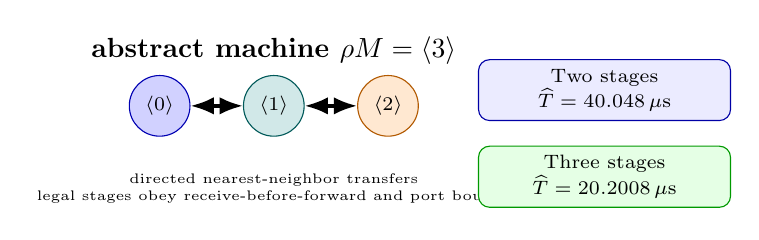
\begin{tikzpicture}[>=Latex,font=\scriptsize]
\node[font=\bfseries] at (1.45,.7) {abstract machine $\rho M=\langle3\rangle$};
\foreach \i/\color in {0/blue,1/teal,2/orange}{
 \node[circle,draw=\color!70!black,fill=\color!18,
       minimum size=.75cm] (p\i) at (\i*1.45,0) {$\langle\i\rangle$};
}
\draw[<->,very thick] (p0)--(p1);
\draw[<->,very thick] (p1)--(p2);
\node[font=\tiny,align=center] at (1.45,-1.05)
 {directed nearest-neighbor transfers\\
  legal stages obey receive-before-forward and port bounds};
\node[draw=blue!65!black,fill=blue!8,rounded corners,
 minimum width=3.2cm,align=center] at (5.65,.2)
 {Two stages\\$\widehat T=40.048\,\mu\mathrm{s}$};
\node[draw=green!60!black,fill=green!10,rounded corners,
 minimum width=3.2cm,align=center] at (5.65,-.9)
 {Three stages\\$\widehat T=20.2008\,\mu\mathrm{s}$};
\end{tikzpicture}
\caption{Step~107's finite-instance counterexample on a three-component
abstract machine. Under the specified heterogeneous directed-link
contention model, the exact minimum-predicted-time schedule uses more
stages. These numbers are \emph{predictions}, not hardware measurements.}
\label{step108:fig:moa-scheduling-counterexample}
\end{figure}

\paragraph{Implementation boundary.}
Together, these modules provide an auditable path from a restricted typed
$\psi$ specification to $\gamma$-addressed code, $\Omega$ ownership,
logical communication, an abstract topology, legal schedules, and conditional
predicted costs.  The interfaces and certificates establish concrete progress
toward a unified MoA compiler.  They do not yet constitute a general automatic
pipeline from arbitrary source programs to globally optimal physical execution.


\subsection{One derivation, multiple realizations}
\label{step108:subsec:moa-portability}

The portability objective is not to disguise hardware differences.
It is to express them explicitly as shaped machine properties and
mapping constraints, while keeping the MoA $\psi$ specification fixed.
A sequential C realization, an OpenMP CPU realization, an OpenACC
accelerator-target source realization, and an MPI-distributed
realization are alternative backends or realization paths; they are
not alternative mathematical definitions of attention.  The
current codebase contains bounded examples of these paths, but
the presence of a backend does not prove that all target machines
execute it successfully or with the predicted performance.

\begin{figure}[t]
\centering
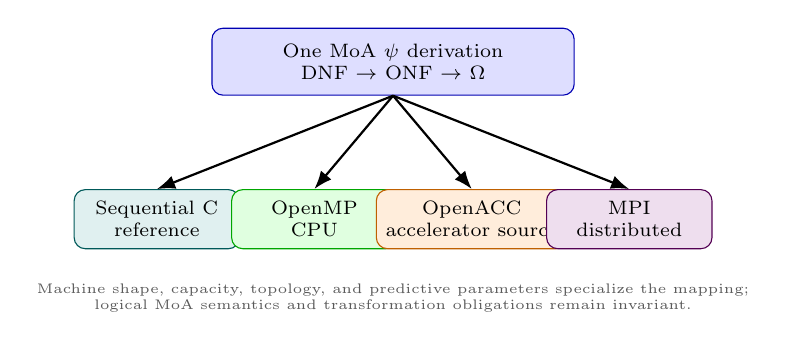
\begin{tikzpicture}[>=Latex,font=\scriptsize,
  root/.style={draw=blue!70!black,fill=blue!13,
     rounded corners,minimum width=4.6cm,minimum height=.85cm,
     align=center},
  backendbox/.style={draw,rounded corners,minimum width=2.1cm,
     minimum height=.75cm,align=center}]
\node[root] (m) at (0,0)
 {One MoA $\psi$ derivation\\DNF $\rightarrow$ ONF $\rightarrow$ $\Omega$};
\node[backendbox,draw=teal!70!black,fill=teal!12] (c)
 at (-3,-2) {Sequential C\\reference};
\node[backendbox,draw=green!65!black,fill=green!12] (omp)
 at (-1,-2) {OpenMP\\CPU};
\node[backendbox,draw=orange!75!black,fill=orange!14] (acc)
 at (1,-2) {OpenACC\\accelerator source};
\node[backendbox,draw=violet!65!black,fill=violet!13] (mpi)
 at (3,-2) {MPI\\distributed};
\foreach \t in {c,omp,acc,mpi}
 \draw[->,thick] (m.south) -- (\t.north);
\node[font=\tiny,align=center,text=black!65] at (0,-3.0)
 {Machine shape, capacity, topology, and predictive parameters
  specialize the mapping;\\logical MoA semantics and
  transformation obligations remain invariant.};
\end{tikzpicture}
\caption{The portable and scalable MoA research goal: a common
mathematical source with target-specific realization and independently
checkable mapping. Backend coverage and hardware validation are
separate empirical questions.}
\label{step108:fig:moa-portable-backends}
\end{figure}

\paragraph{Verifiability as a compiler design principle.}
Each stage must provide a falsifiable obligation: shape legality for
$\psi$; preservation of indexed dependencies in DNF; correct
$\gamma$ addresses in ONF; exact logical ownership under $\Omega$;
resource and communication accounting; topology reachability;
schedule dependency and port legality; and predictive-model
assumptions stated before comparison with measurements.  This
discipline makes compiler outputs auditable, while keeping open the
larger research problem of general semantic equivalence and
performance-optimal compilation.

\paragraph{Research horizon.}
The next milestone is to connect these separately tested components
into one automatic compiler driver and require it to reproduce the
hand-derived MoA attention and Transformer implementations and their
validated behavior.  That is a proposed acceptance criterion, not
a result already demonstrated by the present restricted prototype.


\section{Related work and comparative positioning}
\label{sec:related}
\paragraph{Array and compiler foundations.}
MoA builds on its original array-algebra foundations and subsequent formal and implementation work \cite{mullin1988,hainsmullin1993,mullinjenkins1996,mullin2005,groutmullin2022,markusmullin2024,hainsmullin2026,pythonmoa}. It starts from the semantics of shaped arrays, $\psi$ selection, $\rho$ shape, $\iota$ index generation, and an explicit passage from DNF to $\gamma$-addressed ONF and $\Omega$-lifted machine mappings. This should be evaluated alongside, rather than conflated with, established compiler approaches. The polyhedral model represents affine iteration domains and dependence-preserving schedule transformations \cite{feautrier,pluto}; it offers powerful legality and locality tools but is not the same representation as the MoA normal-form derivation. MLIR supplies extensible intermediate representations and lowering infrastructure \cite{mlir}; it is a plausible implementation substrate, not evidence that a MoA proof or predictor already exists. Halide separates image-processing algorithms from schedules \cite{halide}, and its autoscheduling work addresses the difficult choice of efficient schedules \cite{halideauto}. TVM combines tensor-expression compilation, hardware-aware optimization, and automated search \cite{tvm,ansor}; Triton supplies a GPU programming and compiler system \cite{triton}. None should be characterized as lacking portability or sophisticated scheduling. The distinguishing MoA hypothesis is that one explicit mathematical array semantics can carry checkable index, addressing, mapping, and resource obligations through the entire derivation; its implementation and comparative benefit must be demonstrated, not presumed.

\paragraph{Deep-learning systems and attention kernels.}
PyTorch \cite{pytorch}, TensorFlow \cite{tensorflow}, JAX \cite{jax}, and XLA \cite{xla} provide important reference points for semantics, differentiation, graph compilation, and execution. Transformer attention originates with Vaswani et al.\ \cite{transformer}; memory-efficient implementations include FlashAttention and FlashAttention-2 \cite{flashattention,flashattention2}. Their numerical behavior, memory traffic, fusion, and throughput provide meaningful baselines for an eventual compiler-generated attention implementation. The present paper does not claim to outperform those systems: a fair comparison must align shapes, precision, hardware, compilation, warmup, and end-to-end versus kernel-only measurement. Prior hand-derived MoA attention work \cite{paper1} establishes a reference derivation, but those implementations must not be counted as compiler-generated outputs.

\paragraph{Portable parallel and distributed realization.}
OpenMP \cite{openmp} specifies shared-memory parallel execution and accelerator constructs; OpenACC \cite{openacc} specifies directive-based accelerator programming; MPI \cite{mpi40} specifies message passing across distributed processes, with Open MPI one implementation \cite{openmpi}. Their roles are complementary. The compiler's desired output is a faithful realization of a common $\psi$-indexed computation and its $\gamma$-addressed, $\Omega$-lifted mapping, not a claim that these programming standards themselves derive MoA semantics. Earlier device-specific source generation remains historical evidence of a restricted backend. Portable scalability must be tested with actual OpenMP/OpenACC/MPI programs and documented toolchains, not inferred from portability of the standards alone.

\paragraph{Communication and performance prediction.}
BSP \cite{bsp}, LogP \cite{logp}, and LogGP \cite{loggp} are established abstractions for communication and synchronization costs; Roofline \cite{roofline} and communication-avoiding analysis \cite{ballard} provide complementary resource bounds. The staged link model in Section~\ref{sec:v14communication} is a conditional, schedule-specific estimate, not a new general network-performance theorem or a measured replacement for those models. The earlier Step 102 model omits contention; Step 103 adds logical directed-link contention (Section~\ref{sec:nov-contention-selection}), while physical routing and calibration remain unmodeled. The broader predictive program is developed in \cite{gap}; agreement with measured time and energy on additional hardware remains a separate validation requirement.

\paragraph{Signal-processing comparisons and provenance.}
The accepted CSCI 2026 manuscript \cite{csci} develops MoA-derived image-processing and attention examples. The original signal-processing experiment \cite{signal2026} supplies a controlled Halide realization and frozen prospective validation, while the A40 study \cite{a40report} supplies an MPI/OpenMP-target two-device validation. Section~\ref{sec:signal-evidence} reports the actual evidence with its measurement boundaries. Those implementations were hand-derived, not produced by the compiler described in this paper. Thus they motivate a stringent compiler acceptance test: reproduce the mathematical results, executable mappings, and experimentally observed behavior without retroactively claiming earlier work as generated output.


\subsection{Experimental evidence from MoA-derived signal and image processing}
\label{sec:signal-evidence}
The companion signal-processing study \cite{signal2026} provides a concrete comparison with Halide as an \emph{execution realization}, rather than treating Halide as an unoptimized foil. The experimental sequence separates pointwise Threshold (no semantic cross-owner communication), $3\times3$ Sobel (an index-derived two-row halo), and a heterogeneous Halide Sobel realization. The latter used a frozen CPU--GPU ownership split, $q_C=9537$ and $q_G=252605$ output rows, with an 8192-byte two-row boundary exchange. These quantities follow from the stated index dependencies and ownership, while measured time also depends on the actual CPU affinity and accelerator execution path.

\begin{table}[htbp]\centering\small
\caption{Previously hand-derived signal-processing validation from \cite{signal2026}. Predictions were fixed before the reported validating executions. Times are reported critical-path times for the individual realizations; they are \emph{not} speedup measurements of the present compiler or interchangeable kernel-only benchmarks.}\label{tab:signal-evidence}
\begin{tabular}{p{.29\linewidth}rrr}\toprule
Realization & Frozen (ms) & Measured (ms) & Error (\%)\\\midrule
Threshold, heterogeneous & 86.205582 & 85.816671 & $-0.451$\\
Sobel, OpenMP target & 10.050047 & 10.666868 & $+6.137$\\
Sobel, Halide & 6.495540 & 6.465319 & $-0.4653$\\\bottomrule
\end{tabular}
\end{table}

The Halide experiment reported a checksum of $10{,}528{,}147{,}004$, equal to the expected value. Its controlled CPU placement used eight distinct physical cores after an earlier nominal eight-logical-CPU allocation was found to contain simultaneous-multithreading sibling pairs. The measured GPU-rank median of 6.465319 ms formed the critical path; the CPU-rank median was 5.418318 ms. The original study explicitly cautions that resident-device Halide timings and end-to-end OpenMP-target timings have different data-movement boundaries. We therefore compare \emph{prospective prediction accuracy within each realization}, not relative performance across incomparable timing boundaries.

The complementary A40 study \cite{a40report} derived ownership and communication from the same MoA index semantics, then realized a two-device configuration with MPI ranks and OpenMP target offloading. For its two-GPU pointwise test, the frozen semantic halo prediction was zero bytes; for its two-GPU Sobel test it was 32,768 bytes. The reported executions matched those communication predictions for the tested partition and mapping. These are hand-derived experimental validations, not outputs of the SC27 compiler. They provide independently specified acceptance cases for future automated $\psi$ reduction, $\gamma$ addressing, $\Omega$ lifting, ownership, communication, and source generation.

\paragraph{Why the Halide comparison matters.}
Halide already separates algorithm from schedule \cite{halide,halide2012}. The research distinction is not that Halide cannot optimize image-processing pipelines. Instead, the signal-processing work tests whether MoA index composition, ownership, and measured machine properties can specify required communication and a frozen critical-path prediction before execution. A future compiler-to-Halide or compiler-to-OpenMP/OpenACC/MPI comparison must use matching problem shapes, data residency, hardware, affinity, timing boundaries, and correctness checks. Neither the table above nor the A40 tests establish that the current compiler outperforms Halide.

\begin{table}[htbp]\centering\small
\caption{Positioning by primary mechanism; a comparison of research approaches, not a performance ranking.}\label{tab:related-position}
\begin{tabular}{p{0.19\linewidth}p{0.33\linewidth}p{0.36\linewidth}}\toprule
Approach & Established emphasis & Distinct MoA compiler obligation \\\midrule
Halide / TVM & Algorithm/schedule separation; hardware-aware optimization and search & Derive indexed semantics and explicit addressing/machine-shape certificates \\
MLIR / polyhedral & IR infrastructure; dependence-aware legal transformation & Express and check $\psi$ reduction, DNF, ONF, and $\Omega$ mappings \\
PyTorch / attention kernels & Framework semantics; optimized attention execution & Reproduce reference attention semantics and measure like-for-like resource costs \\
OpenMP / OpenACC / MPI & Portable execution and communication mechanisms & Generate faithful realizations and validate correctness and scaling \\
BSP / LogP / Roofline & Communication and performance abstractions & Predict a specified shaped-machine mapping and validate its error \\\bottomrule
\end{tabular}
\end{table}

\section{Conclusion}
The restricted rewrite pipeline emits CPU, GPU, and coordinated CPU--GPU source from a common attention operation, with subsequent numerical and timing validation on UAlbany DGX hardware (Section~\ref{sec:v13hardware}). The objective is a universal MoA compiler that mechanically derives semantically equivalent coordinated execution across heterogeneous resource ensembles and predicts feasible mappings on a time--energy frontier. MoA provides a principled path from array semantics to operational realization. The scientific contribution pursued here is to automate a derivation chain previously carried out by hand, while maintaining clear correctness and prediction obligations. Initial UAlbany results demonstrate held-out selection and timing validation for a limited empirical model. The logical routing, contention prediction, and candidate-scheduling results establish testable communication structure and conditional time formulas, while OpenMP, OpenACC, and MPI provide the intended portable shared-memory, accelerator, and distributed realization pathways. Historical generated accelerator results remain labeled by their actual implementation; end-to-end OpenACC and MPI performance claims require separately archived tests. Extending deterministic machine-shape theory to predict physical placement, traffic, time, energy, and power remains an open and measurable research objective.
\section*{Acknowledgments}
We acknowledge University at Albany research-computing support and computational resources used in this research program, including resources accessed through NSF ACCESS. Earlier work used ACCESS resources including Stampede, Expanse, Bridges, Purdue Anvil, and NCSA Delta, including AMD GPU resources on Delta. Separate Chameleon Cloud award support enabled Intel GPU energy experiments. Award numbers, system versions, and experiment-level provenance should be verified against the corresponding records before submission.
\begin{thebibliography}{99}
\bibitem{signal2026} L. M. R. Mullin et al., ``Mathematics of Arrays for Huge Heterogeneous Signal and Image Processing: From Semantic Normal Form to Predictive Machine Mapping,'' research manuscript submitted to IPDPS 2027, 2026. The source manuscript provided for this revision documents the heterogeneous Halide Sobel validation; publication status and full author list to be confirmed.
\bibitem{a40report} L. M. R. Mullin et al., ``MoA A40'' two-GPU pointwise and Sobel prospective-validation report, 2026, author-supplied research manuscript. Final title, author list, and publication status to be confirmed.
\bibitem{mullin1988} L. M. R. Mullin, \emph{A Mathematics of Arrays}, Ph.D. dissertation, Syracuse University, 1988. \url{https://surface.syr.edu/eecs_etd/74/}.
\bibitem{hainsmullin1993} G. Hains and L. M. R. Mullin, ``Parallel Functional Programming with Arrays,'' \emph{The Computer Journal}, vol. 36, no. 3, pp. 238--245, 1993.
\bibitem{mullinjenkins1996} L. M. R. Mullin and M. A. Jenkins, ``Effective Data Parallel Computation Using the Psi Calculus,'' \emph{Concurrency: Practice and Experience}, vol. 8, no. 7, pp. 499--515, 1996.
\bibitem{mullin2005} L. Mullin, ``A Uniform Way of Reasoning about Array-Based Computation in Radar: Algebraically Connecting the Hardware/Software Boundary,'' \emph{Digital Signal Processing}, vol. 15, no. 5, pp. 466--520, 2005.
\bibitem{groutmullin2022} I. A. Grout and L. Mullin, ``Realizing Mathematics of Arrays Operations as Custom Architecture Hardware-Software Co-Design Solutions,'' \emph{Information}, vol. 13, no. 11, art. 528, 2022.
\bibitem{markusmullin2024} A. Markus and L. Mullin, ``Implementing Mathematics of Arrays in Modern Fortran: Efficiency and Efficacy,'' \emph{Software}, vol. 3, no. 4, pp. 534--548, 2024.
\bibitem{hainsmullin2026} G. Hains and L. Mullin, ``New Mathematics for Computer Performance: Array Algebra and Cost Functions,'' \emph{Mathematics}, vol. 14, no. 9, art. 1479, 2026.
\bibitem{pythonmoa} C. Ostrouchov and L. Mullin, ``PythonMoA,'' Quansight Labs, 2022. \url{https://github.com/Quansight-Labs/python-moa}.
\bibitem{halide2012} J. Ragan-Kelley et al., ``Decoupling Algorithms from Schedules for Easy Optimization of Image Processing Pipelines,'' \emph{ACM Transactions on Graphics}, vol. 31, no. 4, art. 32, 2012.

\bibitem{paper1} L. M. Mullin and G. Hains, ``Attention at the Theoretical Minimum: A Mathematics of Arrays Framework for Memory-Optimal Transformer Kernels,'' arXiv:2606.07713, 2026.
\bibitem{hetero} L. M. Mullin and G. Hains, ``One Derivation, Any Machine: Deriving a Weighted, Communication-Free Partition for Attention Across a Heterogeneous, Multi-Institution Device Ensemble,'' 2026.
\bibitem{gap} L. M. Mullin and G. Hains, ``Closing the Prediction Gap: Completing Machine Shape So That Predicted Time, Power, Energy, and Mapping Match What Real Hardware Does,'' arXiv:2610.03197, 2026.
\bibitem{csci} L. M. Mullin, ``Mathematics of Arrays: From Invariant Normal Form to Dimension-Lifted Parallel Execution,'' accepted for CSCI 2026, scheduled for December 2026; publication details pending.
\bibitem{halide} J. Ragan-Kelley et al., ``Halide: A Language and Compiler for Optimizing Parallelism, Locality, and Recomputation in Image Processing Pipelines,'' ACM SIGPLAN PLDI, 2013.
\bibitem{halideauto} R. Adams et al., ``Learning to Optimize Halide with Tree Search and Random Programs,'' ACM Transactions on Graphics, 2019.
\bibitem{tvm} T. Chen et al., ``TVM: An Automated End-to-End Optimizing Compiler for Deep Learning,'' USENIX OSDI, 2018.
\bibitem{ansor} L. Zheng et al., ``Ansor: Generating High-Performance Tensor Programs for Deep Learning,'' USENIX OSDI, 2020.
\bibitem{mlir} C. Lattner et al., ``MLIR: Scaling Compiler Infrastructure for Domain Specific Computation,'' IEEE/ACM CGO, 2021.
\bibitem{triton} P. Tillet, H.-T. Kung, and D. Cox, ``Triton: An Intermediate Language and Compiler for Tiled Neural Network Computations,'' ACM MAPL, 2019.
\bibitem{feautrier} P. Feautrier, ``Some Efficient Solutions to the Affine Scheduling Problem. Part I. One-Dimensional Time,'' International Journal of Parallel Programming, 1992.
\bibitem{pluto} U. Bondhugula et al., ``A Practical Automatic Polyhedral Parallelizer and Locality Optimizer,'' ACM SIGPLAN PLDI, 2008.
\bibitem{pytorch} A. Paszke et al., ``PyTorch: An Imperative Style, High-Performance Deep Learning Library,'' NeurIPS, 2019.
\bibitem{tensorflow} M. Abadi et al., ``TensorFlow: A System for Large-Scale Machine Learning,'' USENIX OSDI, 2016.
\bibitem{jax} J. Bradbury et al., ``JAX: Composable Transformations of Python+NumPy Programs,'' 2018, software project, \url{https://github.com/jax-ml/jax}.
\bibitem{xla} OpenXLA Project, ``XLA: Optimizing Compiler for Machine Learning,'' project documentation, \url{https://openxla.org/xla} (accessed 2026).
\bibitem{transformer} A. Vaswani et al., ``Attention Is All You Need,'' NeurIPS, 2017.
\bibitem{flashattention} T. Dao et al., ``FlashAttention: Fast and Memory-Efficient Exact Attention with IO-Awareness,'' NeurIPS, 2022.
\bibitem{flashattention2} T. Dao, ``FlashAttention-2: Faster Attention with Better Parallelism and Work Partitioning,'' ICLR, 2024.
\bibitem{openmp} OpenMP Architecture Review Board, ``OpenMP Application Programming Interface,'' specification, \url{https://www.openmp.org/specifications/}.
\bibitem{openacc} OpenACC Organization, ``OpenACC Application Programming Interface,'' specification, \url{https://www.openacc.org/specification}.
\bibitem{mpi40} Message Passing Interface Forum, ``MPI: A Message-Passing Interface Standard, Version 4.0,'' 2021, \url{https://www.mpi-forum.org/docs/}.
\bibitem{openmpi} Open MPI Project, ``Open MPI: Open Source High Performance Computing,'' project documentation, \url{https://www.open-mpi.org/}.
\bibitem{bsp} L. G. Valiant, ``A Bridging Model for Parallel Computation,'' Communications of the ACM, 1990.
\bibitem{logp} D. Culler et al., ``LogP: Towards a Realistic Model of Parallel Computation,'' ACM SIGPLAN PPOPP, 1993.
\bibitem{loggp} A. Alexandrov et al., ``LogGP: Incorporating Long Messages into the LogP Model,'' Journal of Parallel and Distributed Computing, 1997.
\bibitem{roofline} S. Williams, A. Waterman, and D. Patterson, ``Roofline: An Insightful Visual Performance Model for Multicore Architectures,'' Communications of the ACM, 2009.
\bibitem{ballard} G. Ballard, J. Demmel, O. Holtz, and O. Schwartz, ``Minimizing Communication in Numerical Linear Algebra,'' SIAM Journal on Matrix Analysis and Applications, 2011.
\end{thebibliography}
\end{document}
